% !TeX program = pdflatex
% Informe Técnico - Proyecto Global Integrador AyME
% Archivo base para TeXstudio. Completar los datos marcados con TODO.

\documentclass[10pt,a4paper]{article}

% ---------------------------------------------------------
% PAQUETES
% ---------------------------------------------------------
\usepackage[utf8]{inputenc}
\usepackage[T1]{fontenc}
\usepackage[spanish,es-tabla]{babel}
\usepackage{amsmath,amssymb}
\usepackage{siunitx}
\usepackage{booktabs}
\usepackage{array}
\usepackage{float}
\usepackage{graphicx}
\usepackage{subcaption}
\usepackage{xcolor}
\usepackage{tikz}
\usepackage{fancyhdr}
\usepackage{lastpage}
\usepackage{geometry}
\usepackage{hyperref}
\usepackage{enumitem}

\usetikzlibrary{positioning,arrows.meta}

% ---------------------------------------------------------
% CONFIGURACIÓN GENERAL
% ---------------------------------------------------------
\geometry{
    a4paper,
    left=2.0cm,
    right=2.0cm,
    top=1.70cm,
    bottom=1.5cm,
    headheight=40pt,
    headsep=0.25cm,
    includeheadfoot
}

\sisetup{
    output-decimal-marker={,},
    per-mode=symbol,
    exponent-product=\cdot
}

\hypersetup{
    colorlinks=true,
    linkcolor=black,
    citecolor=black,
    urlcolor=blue
}
\setcounter{secnumdepth}{3}
\setcounter{tocdepth}{3}

\setlength{\parindent}{0pt}
\setlength{\parskip}{4pt}
\renewcommand{\baselinestretch}{1.03}

% ---------------------------------------------------------
% DATOS DEL INFORME - COMPLETAR SI HACE FALTA
% ---------------------------------------------------------
\newcommand{\nombreMateria}{AUTOMÁTICA Y MÁQUINAS ELÉCTRICAS}
\newcommand{\nombreProyecto}{Control de Accionamiento de CA mediante Motor Sincrónico de Imanes Permanentes}
\newcommand{\alumnos}{Ricco Germán (13653), Mamaní Gabriel (13401)}
\newcommand{\anioProyecto}{2026}
\newcommand{\fechaPresentacion}{Julio 2026}
\newcommand{\profesor}{Ing. Gabriel L. Julián}

% ---------------------------------------------------------
% ENCABEZADO Y PIE DE PÁGINA
% ---------------------------------------------------------
\pagestyle{fancy}
\fancyhf{}

% Encabezado en una sola caja de ancho completo para evitar superposiciones.
\newcommand{\encabezadoInforme}{%
    \begin{minipage}[b]{0.30\textwidth}
        \raggedright\scriptsize
        UNCuyo -- Ingeniería Mecatrónica\\[-1pt]
        Mendoza -- Argentina
    \end{minipage}\hfill%
    \begin{minipage}[b]{0.42\textwidth}
        \centering\scriptsize
        Espacio Curricular\\[-1pt]
        \nombreMateria\\[-1pt]
        PROYECTO GLOBAL INTEGRADOR
    \end{minipage}\hfill%
    \begin{minipage}[b]{0.26\textwidth}
        \raggedleft\scriptsize
        Año: \anioProyecto\\[-1pt]
        Alumnos: Ricco -- Mamaní
    \end{minipage}%
}

\fancyhead[L]{\encabezadoInforme}
\fancyhead[C]{}
\fancyhead[R]{}
\fancyfoot[C]{\footnotesize Pág. \thepage\ de \pageref{LastPage}}
\renewcommand{\headrulewidth}{0.4pt}
\renewcommand{\footrulewidth}{0.4pt}

% También aplicamos el mismo formato cuando LaTeX use estilo ``plain''.
\fancypagestyle{plain}{%
    \fancyhf{}
    \fancyhead[L]{\encabezadoInforme}
    \fancyhead[C]{}
    \fancyhead[R]{}
    \fancyfoot[C]{\footnotesize Pág. \thepage\ de \pageref{LastPage}}
    \renewcommand{\headrulewidth}{0.4pt}
    \renewcommand{\footrulewidth}{0.4pt}
}

% ---------------------------------------------------------
% DOCUMENTO
% ---------------------------------------------------------
\begin{document}

% ---------------------------------------------------------
% CARÁTULA
% ---------------------------------------------------------
\begin{titlepage}
    \thispagestyle{empty}
    \centering

    \vspace*{0.7cm}

    {\large UNCuyo -- Ingeniería Mecatrónica\\[2pt]
    Facultad de Ingeniería -- Universidad Nacional de Cuyo\\[2pt]
    Mendoza -- Argentina}\par

    \vspace{1.1cm}

    {\Large \textbf{Espacio Curricular:}}\par
    {\Large \textbf{\nombreMateria}}\par

    \vspace{1.6cm}

    {\Huge \textbf{Proyecto Global Integrador}}\par

    \vspace{1.0cm}

    \begin{minipage}{0.92\textwidth}
        \centering
        {\LARGE\bfseries Control de Accionamiento de CA\\[6pt]
        mediante Motor Sincrónico de Imanes Permanentes\par}
    \end{minipage}

    \vfill

    \begin{tabular}{rl}
        \textbf{Alumnos:} & \alumnos \\
        \textbf{Profesor Titular:} & \profesor \\
        \textbf{Año:} & \anioProyecto \\
        \textbf{Fecha de presentación:} & \fechaPresentacion \\
    \end{tabular}

    \vspace*{0.8cm}
\end{titlepage}

% ---------------------------------------------------------
% Desde aquí comienza el informe propiamente dicho, con encabezado y pie.
% -------------------------------------------------------- 

\clearpage
\setcounter{page}{1}
\pagestyle{fancy}

% ---------------------------------------------------------
% RESUMEN
% ---------------------------------------------------------
\section{Resumen}
\addcontentsline{toc}{section}{Resumen}

En este informe se desarrolla el modelado, análisis, simulación y posterior diseño de control de un accionamiento electromecánico de corriente alterna basado en un motor sincrónico de imanes permanentes. El sistema bajo estudio está compuesto por una máquina PMSM trifásica alimentada por un inversor, acoplada mediante una transmisión planetaria a una carga mecánica equivalente de un grado de libertad. El objetivo general del proyecto es obtener un modelo dinámico del sistema físico, analizar su comportamiento a lazo abierto y diseñar posteriormente una estrategia de control de movimiento en cascada con control vectorial.

En esta etapa se presenta la definición del sistema y se desarrolla el modelo matemático equivalente del subsistema mecánico completo, compuesto por el rotor del motor, la transmisión rígida y la carga. Luego se incorpora el subsistema electromagnético de la PMSM en coordenadas \(qd0\), junto con el modelo térmico del bobinado de estator. Se obtiene el modelo dinámico global no lineal, su linealización Jacobiana en un punto genérico de operación y un modelo LTI equivalente aumentado mediante linealización por retroalimentación, imponiendo la condición de campo orientado \(i_{ds}^{r}(t)\equiv0\). Este desarrollo constituye la base para los análisis posteriores de estabilidad, controlabilidad, observabilidad y diseño del controlador de movimiento.

\textit{Nota: este resumen debe actualizarse al finalizar el informe completo, incorporando los resultados de simulación, control y conclusiones finales.}

% ---------------------------------------------------------
% INTRODUCCIÓN
% ---------------------------------------------------------
\section{Introducción}

El presente Proyecto Global Integrador tiene como objetivo aplicar los contenidos de Automática y Máquinas Eléctricas al modelado y control de un sistema mecatrónico simplificado. El sistema estudiado corresponde a un accionamiento de corriente alterna de cuatro cuadrantes, basado en un motor sincrónico de imanes permanentes (PMSM) alimentado por un inversor trifásico y acoplado a una carga mecánica mediante una caja reductora planetaria. La variable principal a controlar será la posición angular de la carga, considerando además los efectos de fricción, gravedad, perturbaciones externas, dinámica eléctrica y calentamiento del bobinado.

El trabajo se organiza siguiendo la guía del Proyecto Global Integrador \cite{guia_trabajo}. En primer lugar se obtiene el modelo mecánico equivalente del actuador, la transmisión y la carga, referido al eje del motor. Luego se incorpora el modelo electromagnético de la PMSM, las transformaciones de Park, el modelo térmico, la linealización del sistema y el modelo LTI equivalente para análisis. En las secciones posteriores se desarrollarán el análisis de estabilidad, controlabilidad y observabilidad, el diseño del control vectorial y del controlador de movimiento, la implementación discreta y la verificación mediante simulaciones. La estructura y el formato general del presente informe siguen los lineamientos indicados por la cátedra para la presentación del Informe Técnico \cite{guia_informe}.

% ---------------------------------------------------------
% DESARROLLO
% ---------------------------------------------------------
\section{Modelado, Análisis y Simulación dinámica del SISTEMA FÍSICO a Lazo Abierto}

\subsection{Definición del sistema bajo estudio}

El sistema físico analizado está compuesto por los siguientes subsistemas principales:

\begin{itemize}[leftmargin=*]
    \item Subsistema mecánico del motor, representado por la inercia del rotor y su fricción viscosa equivalente.
    \item Transmisión rígida mediante caja reductora planetaria, caracterizada por una relación de transmisión constante.
    \item Carga mecánica de un grado de libertad, modelada como un péndulo rígido actuado en el plano vertical.
    \item Subsistema electromagnético de la máquina PMSM, que será incorporado en las siguientes etapas del informe.
    \item Subsistema térmico del bobinado del estator, asociado principalmente a las pérdidas por efecto Joule.
    \item Inversor trifásico y sensores de corriente, posición y temperatura, considerados posteriormente para la implementación del sistema de control.
\end{itemize}

La primera etapa del desarrollo consiste en obtener un modelo mecánico equivalente que permita representar al motor, la caja reductora y la carga como un único sistema dinámico referido al eje del motor. Esta compactación es conveniente porque el torque electromagnético de la PMSM actúa sobre el eje del motor, mientras que la variable de interés del proceso es la posición angular de la carga.

\subsection{Modelo matemático del subsistema mecánico}

En esta sección se obtiene el modelo matemático equivalente de un grado de libertad del subsistema mecánico completo. Para ello se modelan por separado la carga, la transmisión y el eje mecánico del motor, y luego se reflejan las variables de la carga al eje del motor.

El modelado se realiza bajo las siguientes hipótesis:

\begin{itemize}[leftmargin=*]
    \item La transmisión se considera rígida e ideal.
    \item No se considera elasticidad torsional.
    \item No se considera juego mecánico o \textit{backlash}.
    \item No se consideran pérdidas adicionales en la transmisión.
    \item La carga se modela como un péndulo rígido actuado en el plano vertical.
    \item La fricción se modela como viscosa.
\end{itemize}

% -------------------------------------
\subsubsection{Carga mecánica}

La carga mecánica se modela como un sistema rotacional de un grado de libertad, cuya coordenada articular es $q(t)$.
Aplicando la segunda ley de Newton para movimiento rotacional, se obtiene la ecuación fundamental de la carga:

\begin{equation}
    J_l \ddot{q}(t) = T_q(t) - b_l \dot{q}(t) - T_l(t)
    \label{eq:carga_mecanica}
\end{equation}

% Explicacion de Terminos
donde 
$J_l$ es el momento de inercia total de la carga referido al eje de la articulación, 
\(b_l\) es el coeficiente de fricción viscosa de la carga, 
\(T_q(t)\) es el torque aplicado por la salida de la caja reductora y 
\(T_l(t)\) es el torque resistente total aplicado sobre la carga.

El torque resistente de carga $T_l(t)$ se compone de un término gravitacional y una perturbación externa $T_{ld}(t)$ aplicada sobre la articulacion:

\begin{equation}
    T_l(t) = g k_l \sin(q(t)) + T_{ld}(t)
    \label{eq:torque_carga}
\end{equation}

donde $g$ es la aceleración de la gravedad. Los parámetros equivalentes gravitacional ($k_l$) e inercial ($J_l$) 
de la carga se definen a partir de la geometría y masa del sistema como:

\begin{equation*}
    k_l = m L_{cm} + m_l L_l
\end{equation*}
\begin{equation*}
    J_l = m L_{cm}^{2} + J_{cm} + m_l L_l^{2}
\end{equation*}

% Explicacion de terminos
siendo $m$ y $J_{cm}$ la masa y el momento de inercia propio del eslabón (respecto a su centro de masa), 
$L_{cm}$ la distancia desde la articulación a dicho centro, 
$m_l$ la masa de la carga útil, 
y $L_l$ la longitud total del eslabón.

% -------------------------------------
\subsubsection{Tren de transmisión}

El motor se encuentra acoplado a la carga mediante una caja reductora de relación de transmisión $r$.
Al considerarse ideal y rígida, las relaciones cinemáticas y de transmisión de torque se agrupan en el siguiente sistema:

\begin{equation}
    \begin{aligned}
        q(t) &= \frac{1}{r}\theta_m(t), \\
        \dot{q}(t) &= \frac{1}{r}\omega_m(t), \\
        T_q(t) &= r T_d(t),
    \end{aligned}
    \label{eq:transmision}
\end{equation}

donde \(\omega_m(t)\) y \(\theta_m(t)\) son la velocidad angular y posición angular del rotor del motor,
y $T_d(t)$ representa el torque resistente reflejado por la transmisión sobre el eje del motor.

% -------------------------------------
\subsubsection{Subsistema mecánico del motor}

La dinámica mecánica del rotor del motor PMSM, referida a su propio eje, se expresa mediante sus variables de estado cinemáticas:

\begin{equation}
    \begin{aligned}
        \dot{\theta}_m(t) &= \omega_m(t), \\
        J_m \dot{\omega}_m(t) &= T_m(t) - b_m \omega_m(t) - T_d(t),
    \end{aligned}
    \label{eq:mecanica_motor}
\end{equation}

% Explicacion de Terminos
donde $J_m$ representa la inercia propia del rotor sumada a la inercia equivalente de la caja reductora (referida al eje del motor), 
$b_m$ es el coeficiente de fricción viscosa de dicho eje, 
y $T_m(t)$ es el torque electromagnético generado por la máquina.

% -------------------------------------
\subsubsection{Obtención del modelo equivalente referido al eje del motor}

Para obtener el modelo equivalente referido al eje del motor, se reemplazan las relaciones de transmisión \eqref{eq:transmision} 
en la ecuación de la carga \eqref{eq:carga_mecanica}. Como la relación de transmisión es constante, sus derivadas temporales resultan:

\begin{equation*}
    \begin{aligned}
        q(t) &= \frac{\theta_m(t)}{r}, \\
        \dot{q}(t) &= \frac{\omega_m(t)}{r}, \\
        \ddot{q}(t) &= \frac{\dot{\omega}_m(t)}{r}.
    \end{aligned}
\end{equation*}

Reemplazando en \eqref{eq:carga_mecanica} se obtiene:

\begin{equation*}
    J_l \frac{\dot{\omega}_m(t)}{r} = r T_d(t) - b_l \frac{\omega_m(t)}{r} - T_l(t).
\end{equation*}

Despejando el torque resistente reflejado $T_d(t)$, se tiene:

\begin{equation*}
    T_d(t) = \frac{J_l}{r^2}\dot{\omega}_m(t) + \frac{b_l}{r^2}\omega_m(t) + \frac{T_l(t)}{r}.
\end{equation*}

Sustituyendo esta expresión en la dinámica mecánica del motor \eqref{eq:mecanica_motor}, resulta:

\begin{equation*}
    J_m \dot{\omega}_m(t) = T_m(t) - b_m \omega_m(t) - \left[ \frac{J_l}{r^2}\dot{\omega}_m(t) + \frac{b_l}{r^2}\omega_m(t) + \frac{T_l(t)}{r} \right].
\end{equation*}

Agrupando términos, la ecuación se puede reescribir como:

\begin{equation*}
    \left( J_m + \frac{J_l}{r^2} \right) \dot{\omega}_m(t) = T_m(t) - \left( b_m + \frac{b_l}{r^2} \right) \omega_m(t) - \frac{T_l(t)}{r}.
\end{equation*}

A partir de esta expresión, se definen los parámetros equivalentes referidos al eje del motor:

\begin{equation*}
    J_{eq} = J_m + \frac{J_l}{r^2}, \qquad b_{eq} = b_m + \frac{b_l}{r^2}, \qquad T_{eq}(t) = \frac{T_l(t)}{r}.
\end{equation*}

Sustituyendo el torque de carga por su expresión completa dada en \eqref{eq:torque_carga}, el torque equivalente de carga referido al eje del motor resulta:

\begin{equation*}
    T_{eq}(t) = \frac{g k_l}{r} \sin\left(\frac{\theta_m(t)}{r}\right) + \frac{T_{ld}(t)}{r}.
\end{equation*}

Finalmente, el modelo mecánico equivalente referido al eje del motor queda definido por el siguiente sistema:

\begin{equation}
    \begin{aligned}
        \dot{\theta}_m(t) &= \omega_m(t), \\
        J_{eq}\dot{\omega}_m(t) &= T_m(t) - b_{eq}\omega_m(t) - \frac{g k_l}{r} \sin\left(\frac{\theta_m(t)}{r}\right) - \frac{T_{ld}(t)}{r}.
    \end{aligned}
    \label{eq:modelo_mecanico_final}
\end{equation}

La salida mecánica de interés, correspondiente a la posición angular de la articulación, es:

\begin{equation}
    q(t) = \frac{\theta_m(t)}{r}.
    \label{eq:salida_articulacion}
\end{equation}

% ----------------------------------------------------
\subsubsection{Justificación de la compactación mecánica}

La compactación del subsistema mecánico en un único modelo de un grado de libertad es posible debido a que la transmisión se asume rígida, ideal y sin pérdidas. 
En consecuencia, existe una relación cinemática fija y proporcional entre el eje del motor y el eje de salida. 
A su vez, la relación de transmisión ideal permite reflejar de forma directa los torques.

Bajo estas condiciones, la inercia y la fricción propias de la carga se reflejan al eje del motor multiplicadas por el factor $1/r^2$, 
mientras que los torques externos (como la gravedad y las perturbaciones) aplicados sobre la carga se reflejan escalados por el factor $1/r$. 
De esta forma, el motor, la transmisión y la carga pueden representarse matemáticamente como un único sistema mecánico equivalente referido al eje motriz.

% ----------------------------------------------------
\subsubsection{Modelo en espacio de estados}

Definiendo como variables de estado a la posición angular y la velocidad del rotor, es decir, 
$x_1(t)=\theta_m(t)$ y $x_2(t)=\omega_m(t)$, el modelo mecánico equivalente queda representado por el siguiente sistema dinámico no lineal:

\begin{equation}
    \boxed{
    \begin{aligned}
        \dot{x}_1(t) &= x_2(t), \\
        \dot{x}_2(t) &= \frac{1}{J_{eq}} \left[ T_m(t) - b_{eq}x_2(t) - \frac{g k_l}{r} \sin\left(\frac{x_1(t)}{r}\right) - \frac{T_{ld}(t)}{r} \right], \\
        y(t) &= q(t) = \frac{x_1(t)}{r}.
    \end{aligned}
    }
    \label{eq:ss_mecanico}
\end{equation}

% ----------------------------------------------------
\subsubsection{Diagrama de bloques del subsistema mecánico equivalente}

A partir de las ecuaciones de estado \eqref{eq:ss_mecanico}, se construye el diagrama de bloques del subsistema mecánico equivalente, ilustrado en la Fig. \ref{fig:diagrama_mecanico_equivalente}.
\begin{figure}[H]
    \centering
   	% Inserta la ruta y nombre exacto de tu archivo PNG aquí
   	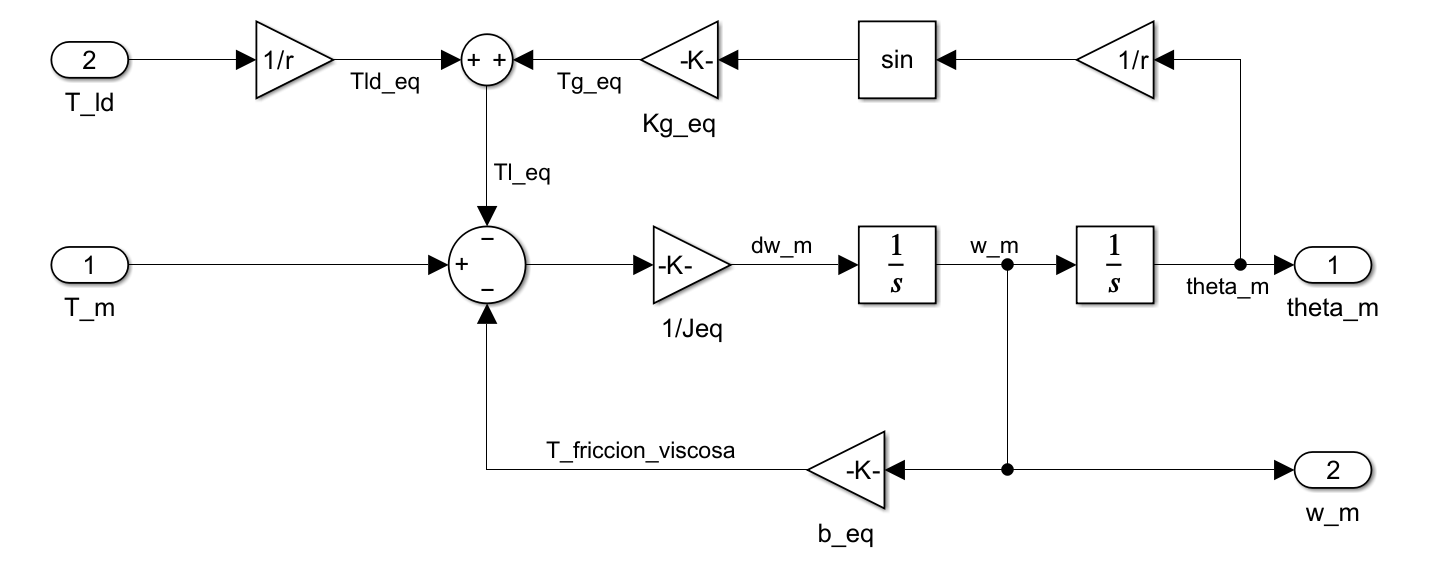
\includegraphics[width=0.95\textwidth]{img/screenshot_subsistema_mecanico.png}
   	\caption{Diagrama de bloques del subsistema mecánico equivalente referido al eje del motor.}
   	\label{fig:diagrama_mecanico_equivalente}
   \end{figure}

El bloque equivalente, implementado mediante parámetros concentrados nominales, 
tiene como entrada principal el torque electromagnético $T_m(t)$, 
como perturbación externa el torque $T_{ld}(t)$, 
y como salida de interés la posición articular $q(t)$. 
La no linealidad geométrica del modelo se concentra en el cálculo del término gravitacional $\sin(\theta_m/r)$.

% ----------------------------------------------------
\subsubsection{Parámetros mecánicos base y ecuaciones de equivalencia}

Los parámetros físicos fundamentales que caracterizan a los distintos componentes del subsistema mecánico se resumen en la Tabla \ref{tab:parametros_mecanicos}.

\begin{table}[H]
    \centering
    \caption{Parámetros nominales del subsistema mecánico.}
    \label{tab:parametros_mecanicos}
    \begin{tabular}{lll}
        \toprule
        Parámetro & Descripción & Valor nominal \\
        \midrule
        $g$ & Aceleración de la gravedad & \(\SI{9.80665}{\meter\per\second\squared}\) \\
        $r$ & Relación de transmisión & \(120\) \\
        $J_m$ & Inercia del motor y caja referida al motor & \(\SI{14.0e-6}{\kilogram\meter\squared}\) \\
        $b_m$ & Fricción viscosa del motor & \(\SI{15.0e-6}{\newton\meter\second\per\radian}\) \\
        $m$ & Masa del eslabón & \(\SI{1.0}{\kilogram}\) \\
        $L_{cm}$ & Distancia al centro de masa del eslabón & \(\SI{0.25}{\meter}\) \\
        $J_{cm}$ & Inercia del eslabón respecto de su centro de masa & \(\SI{0.0208}{\kilogram\meter\squared}\) \\
        $L_l$ & Longitud del eslabón & \(\SI{0.50}{\meter}\) \\
        $m_l$ & Masa de carga útil nominal & \(\SI{0}{\kilogram}\) \\
        $b_l$ & Fricción viscosa de la carga & \(\SI{0.1}{\newton\meter\second\per\radian}\) \\
        $T_{ld,max}$ & Perturbación externa máxima en la carga & \(\SI{5}{\newton\meter}\) \\
        \bottomrule
    \end{tabular}
\end{table}

A partir de estas propiedades físicas, la inercia propia de la carga ($J_l$) y su coeficiente gravitacional ($k_l$) 
quedan definidos analíticamente en función de la masa de carga útil ($m_l$) como:

\begin{equation*}
    \begin{aligned}
        J_l &= m L_{cm}^{2} + J_{cm} + m_l L_l^{2}, \\
        k_l &= m L_{cm} + m_l L_l.
    \end{aligned}
\end{equation*}

Reflejando los efectos dinámicos a través de la transmisión, el conjunto de parámetros equivalentes referidos al eje del motor resulta:

\begin{equation*}
    \begin{aligned}
        J_{eq} &= J_m + \frac{J_l}{r^2}, \\
        b_{eq} &= b_m + \frac{b_l}{r^2}, \\
        T_{g,eq} &= \frac{g k_l}{r}, \\
        T_{ld,eq,max} &= \frac{T_{ld,max}}{r}.
    \end{aligned}
\end{equation*}

% ---------------------------------------------------
\subsubsection{Cálculo de parámetros equivalentes y análisis de incertidumbre}

El sistema real está sujeto a variaciones operativas e incertidumbres paramétricas. 
Específicamente, la masa de carga útil puede variar entre condiciones de vacío y plena carga ($m_l \in [0,\;1.5]\ \si{\kilogram}$), 
lo cual afecta directamente a la inercia total y al torque gravitacional. 
Adicionalmente, se considera una incertidumbre operativa en la fricción viscosa de la carga dada por $b_l = 0.1 \pm 0.03\ \si{\newton\meter\second\per\radian}$.

Para caracterizar matemáticamente la planta de cara a la sintonía del controlador y evaluación de robustez, se calcularon mediante rutinas de \textit{software} (MATLAB) los valores nominales (asumiendo $m_l = \SI{0}{\kilogram}$) y los rangos operativos extremos (mínimo y máximo) para cada parámetro equivalente. 
Los resultados consolidados se sintetizan en la Tabla \ref{tab:parametros_equivalentes_rangos}.

\begin{table}[H]
    \centering
    \caption{Parámetros equivalentes referidos al eje motriz: Valores nominales y rangos de variación.}
    \label{tab:parametros_equivalentes_rangos}
    \resizebox{\textwidth}{!}{
    \begin{tabular}{lllll}
        \toprule
        Parámetro & Expresión analítica & Valor Nominal ($m_l=0$) & Rango Operativo (Mín -- Máx) & Unidad \\
        \midrule
        $J_l$ & $m L_{cm}^{2} + J_{cm} + m_l L_l^2$ & $8.330\times10^{-2}$ & $8.330\times10^{-2}$ -- $4.583\times10^{-1}$ & \si{\kilogram\meter\squared} \\
        $k_l$ & $m L_{cm} + m_l L_l$ & $2.500\times10^{-1}$ & $2.500\times10^{-1}$ -- $1.000$ & \si{\kilogram\meter} \\
        $J_{eq}$ & $J_m + J_l/r^2$ & $1.978\times10^{-5}$ & $1.978\times10^{-5}$ -- $4.582\times10^{-5}$ & \si{\kilogram\meter\squared} \\
        $b_{eq}$ & $b_m + b_l/r^2$ & $2.194\times10^{-5}$ & $1.986\times10^{-5}$ -- $2.403\times10^{-5}$ & \si{\newton\meter\second\per\radian} \\
        $T_{g,eq}$ & $g k_l/r$ & $2.043\times10^{-2}$ & $2.043\times10^{-2}$ -- $8.172\times10^{-2}$ & \si{\newton\meter} \\
        $T_{ld,eq}$ & $T_{ld,max}/r$ & $4.167\times10^{-2}$ & Constante & \si{\newton\meter} \\
        \bottomrule
    \end{tabular}
    }
\end{table}

\subsubsection*{Síntesis del Modelo Mecánico}

A partir de las ecuaciones fundamentales de la carga, la transmisión y el rotor, 
se obtuvo un modelo mecánico compacto referido al eje del motor. 
Este modelo conserva como variables de estado principales la posición y velocidad del rotor, 
e incorpora la dinámica de la carga a través de los parámetros equivalentes de inercia y fricción analizados. 
Este resultado es fundamental, ya que permite utilizar el torque electromagnético $T_m(t)$ como entrada mecánica directa del subsistema, 
lo cual establece el punto de acoplamiento exacto con las ecuaciones electromagnéticas de la máquina PMSM que se desarrollarán a continuación.


% ---------------------------------------------------------
% PUNTO 2 DE LA CONSIGNA
% ---------------------------------------------------------

\subsection{Modelo dinámico del sistema físico completo}

En esta sección se incorpora, al modelo mecánico equivalente obtenido previamente, el subsistema electromagnético de la máquina PMSM y el subsistema térmico del bobinado de estator. El objetivo es pasar de una planta mecánica excitada por un torque genérico \(T_m(t)\) a un modelo físico completo donde dicho torque se obtiene a partir de las corrientes internas de la máquina, las tensiones aplicadas por el inversor y la temperatura del estator.

Para el desarrollo primero se obtiene el modelo global no lineal en coordenadas virtuales \(qd0\), luego se realiza la linealización Jacobiana para obtener un modelo LPV, y finalmente se construye un modelo LTI equivalente mediante linealización por retroalimentación no lineal y control vectorial con campo orientado.

% ---------------------------------------------------------
\subsubsection{Modelo global NO LINEAL del sistema físico completo}

Se busca obtener un modelo dinámico global no lineal del accionamiento completo, incorporando la dinámica mecánica equivalente, la dinámica electromagnética de la máquina PMSM y la dinámica térmica del estator. En esta primera formulación no se impone la condición de campo orientado, por lo que se considera el caso general donde la corriente del eje directo no es nula ($i_{ds}^{r}(t)\neq 0$). Además, para escribir el modelo en coordenadas $qd0$ de forma completa, se conserva inicialmente la componente homopolar $i_{0s}(t)$ como variable de estado. Luego, si se asume conexión estatórica en estrella con neutro flotante y alimentación trifásica equilibrada, puede imponerse la restricción particular $i_{0s}(t)\equiv 0$ y $v_{0s}(t)\equiv 0$, reduciendo el orden del modelo.

\begin{equation*}
	i_{ds}^{r}(t)\neq 0, \qquad i_{0s}(t) \; \text{genérico}.
\end{equation*}


\paragraph{Transformaciones de Park y variables reales.}
El modelo electromagnético se desarrolla en coordenadas virtuales de rotor $qd0$. En este marco de referencia rotórico, las variables eléctricas trifásicas se expresan mediante componentes de eje en cuadratura, eje directo y componente homopolar. Esto simplifica el análisis dinámico y permite representar el acoplamiento entre el inversor, la máquina eléctrica y la mecánica del rotor. Sin embargo, las tensiones y corrientes físicamente accesibles en el inversor y en los sensores son las señales reales de fase del estator $abc$, por lo que deben incorporarse explícitamente las transformaciones de Park directa e inversa.

Definiendo un vector genérico de variables trifásicas $\mathbf{f}_{abcs}(t) = \begin{bmatrix} f_{as}(t) & f_{bs}(t) & f_{cs}(t) \end{bmatrix}^{T}$, el cual puede representar tensiones, corrientes o flujos concatenados, se adopta la transformación de Park directa invariante en amplitud:

\begin{equation*}
	\begin{bmatrix}
		f_{qs}^{r}(t)\\
		f_{ds}^{r}(t)\\
		f_{0s}(t)
	\end{bmatrix}
	=
	\frac{2}{3}
	\begin{bmatrix}
		\cos\theta_r & \cos\left(\theta_r-\frac{2\pi}{3}\right) & \cos\left(\theta_r+\frac{2\pi}{3}\right)\\
		\sin\theta_r & \sin\left(\theta_r-\frac{2\pi}{3}\right) & \sin\left(\theta_r+\frac{2\pi}{3}\right)\\
		\frac{1}{2} & \frac{1}{2} & \frac{1}{2}
	\end{bmatrix}
	\begin{bmatrix}
		f_{as}(t)\\
		f_{bs}(t)\\
		f_{cs}(t)
	\end{bmatrix}.
\end{equation*}

En el presente trabajo, este bloque recibe como entradas las tres variables de fase \(f_a\), \(f_b\), \(f_c\), junto con el ángulo eléctrico del rotor \(\theta_r\), y entrega como salidas las componentes \(f_q^r\), \(f_d^r\) y \(f_0\).

La Fig.~\ref{fig:park_directa_impl} muestra la implementación de la transformación de Park directa mediante un bloque \textit{MATLAB Function}. A la izquierda se observa la interfaz del bloque utilizado en Simulink, mientras que a la derecha se presenta el código interno programado para realizar la conversión \(abc \rightarrow qd0\).

\begin{figure}[H]
	\centering
	
	\begin{minipage}{0.55\textwidth}
		\centering
		
		\begin{subfigure}[t]{0.34\linewidth}
			\centering
			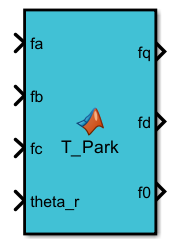
\includegraphics[width=\linewidth]{img/bloque_park_directa.png}
			\caption{Bloque Simulink.}
			\label{fig:bloque_park_directa}
		\end{subfigure}
		\hfill
		\begin{subfigure}[t]{0.62\linewidth}
			\centering
			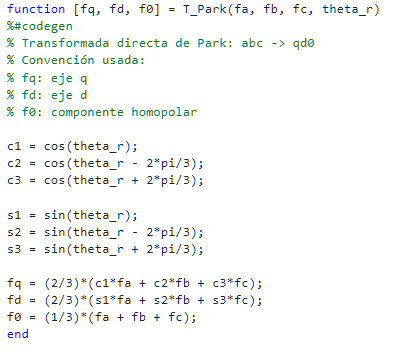
\includegraphics[width=\linewidth]{img/codigo_park_directa.png}
			\caption{Código interno del bloque.}
			\label{fig:codigo_park_directa}
		\end{subfigure}
		
	\end{minipage}
	
	\caption{Implementación de la transformación de Park directa \(abc \rightarrow qd0\) mediante un bloque \textit{MATLAB Function}.}
	\label{fig:park_directa_impl}
\end{figure}

A partir de esta implementación, las variables trifásicas medidas en el sistema real o generadas en la simulación pueden transformarse al marco de referencia rotórico, donde las componentes en régimen permanente se comportan como señales continuas o de variación lenta. Esto simplifica notablemente el análisis dinámico de la máquina y el diseño de estrategias de control orientado a campo.

Para reconstruir las señales físicas de fase a partir de las acciones de control calculadas en el marco virtual, se utiliza la transformación de Park inversa:

\begin{equation*}
	\begin{bmatrix}
		f_{as}(t)\\
		f_{bs}(t)\\
		f_{cs}(t)
	\end{bmatrix}
	=
	\begin{bmatrix}
		\cos\theta_r & \sin\theta_r & 1\\
		\cos\left(\theta_r-\frac{2\pi}{3}\right) & \sin\left(\theta_r-\frac{2\pi}{3}\right) & 1\\
		\cos\left(\theta_r+\frac{2\pi}{3}\right) & \sin\left(\theta_r+\frac{2\pi}{3}\right) & 1
	\end{bmatrix}
	\begin{bmatrix}
		f_{qs}^{r}(t)\\
		f_{ds}^{r}(t)\\
		f_{0s}(t)
	\end{bmatrix}.
\end{equation*}


 En este trabajo, dicha transformación resulta necesaria para reconstruir las señales físicas de fase que posteriormente se aplican al inversor o se utilizan para la representación de variables en el marco real del estator.

El bloque implementado recibe como entradas las componentes \(f_q^r\), \(f_d^r\), \(f_0\) y el ángulo eléctrico del rotor \(\theta_r\), y entrega como salidas las variables de fase \(f_a\), \(f_b\) y \(f_c\).

La Fig.~\ref{fig:park_inversa_impl} muestra la implementación de la transformación de Park inversa.

\begin{figure}[H]
	\centering
	
	\begin{minipage}{0.55\textwidth}
		\centering
		
		\begin{subfigure}[t]{0.34\linewidth}
			\centering
			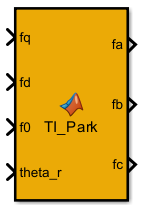
\includegraphics[width=\linewidth]{img/bloque_park_inversa.png}
			\caption{Bloque Simulink.}
			\label{fig:bloque_park_inversa}
		\end{subfigure}
		\hfill
		\begin{subfigure}[t]{0.62\linewidth}
			\centering
			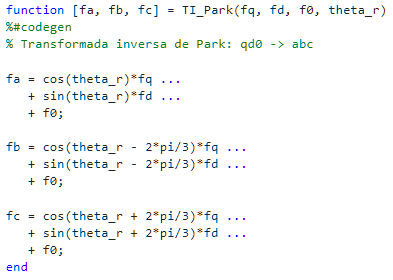
\includegraphics[width=\linewidth]{img/codigo_park_inversa.png}
			\caption{Código interno del bloque.}
			\label{fig:codigo_park_inversa}
		\end{subfigure}
		
	\end{minipage}
	
	\caption{Implementación de la transformación de Park inversa \(qd0 \rightarrow abc\) mediante un bloque \textit{MATLAB Function}.}
	\label{fig:park_inversa_impl}
\end{figure}

La implementación explícita de la transformación inversa permite cerrar de forma coherente el esquema de control vectorial, ya que las acciones de control calculadas en el sistema \(qd0\) pueden ser reinterpretadas en términos de magnitudes físicas trifásicas.

La transformación requiere conocer instantáneamente la posición eléctrica del rotor $\theta_r(t)$, la cual se relaciona con la cinemática mecánica mediante el número de pares de polos $P_p$ de la máquina:

\begin{equation*}
	\theta_r(t) = P_p \theta_m(t), \qquad \omega_r(t) = P_p \omega_m(t).
\end{equation*}



\paragraph{Torque electromagnético.}
El torque electromagnético generado por la máquina PMSM está dado por la interacción entre los flujos magnéticos y las corrientes del estator:

\begin{equation}
	T_m(t) = \frac{3}{2}P_p \lambda_m^{\prime r} i_{qs}^{r}(t) + \frac{3}{2}P_p \left(L_d - L_q\right) i_{ds}^{r}(t)i_{qs}^{r}(t).
	\label{eq:torque_electromagnetico_PMSM}
\end{equation}

El primer término corresponde al torque producido por el flujo de los imanes permanentes del rotor ($\lambda_m^{\prime r}$, referido al estator). El segundo término corresponde al torque de reluctancia, originado por la saliencia magnética del rotor, donde $L_d$ y $L_q$ son las inductancias propias de los ejes directo y en cuadratura respectivamente.

Agrupando constantes, se definen la constante de torque de los imanes $K_t$ y la constante de reluctancia $K_{rel}$:

\begin{equation*}
	K_t = \frac{3}{2}P_p \lambda_m^{\prime r}, \qquad K_{rel} = \frac{3}{2}P_p \left(L_d - L_q\right).
\end{equation*}

Por lo tanto:

\begin{equation}
	T_m(t) = K_t i_{qs}^{r}(t) + K_{rel} i_{ds}^{r}(t)i_{qs}^{r}(t).
	\label{eq:torque_kt_krel}
\end{equation}

El producto cruzado $i_{ds}^{r}(t)i_{qs}^{r}(t)$ constituye una de las no linealidades estructurales del modelo global.

\paragraph{Ecuaciones eléctricas en coordenadas $qd0$.}
Aplicando la Segunda Ley de Kirchhoff a los devanados del estator en el marco de referencia rotórico, el balance dinámico de tensiones queda definido por:

\begin{equation}
	\begin{aligned}
		v_{qs}^{r}(t) &= R_s\left(T_s^{\circ}\right)i_{qs}^{r}(t) + L_q \frac{di_{qs}^{r}(t)}{dt} + \left[\lambda_m^{\prime r} + L_d i_{ds}^{r}(t)\right]\omega_r(t), \\
		v_{ds}^{r}(t) &= R_s\left(T_s^{\circ}\right)i_{ds}^{r}(t) + L_d \frac{di_{ds}^{r}(t)}{dt} - L_q i_{qs}^{r}(t)\omega_r(t), \\
		v_{0s}(t) &= R_s\left(T_s^{\circ}\right)i_{0s}(t) + L_{ls}\frac{di_{0s}(t)}{dt}.
	\end{aligned}
	\label{eq:dinamica_tensiones_qd0}
\end{equation}

Despejando las derivadas de corriente y sustituyendo $\omega_r(t)=P_p\omega_m(t)$, se obtiene:

\begin{equation}
	\begin{aligned}
		\frac{di_{qs}^{r}}{dt} &= \frac{1}{L_q}\left[v_{qs}^{r} - R_s\left(T_s^{\circ}\right)i_{qs}^{r} - \left(\lambda_m^{\prime r}+L_d i_{ds}^{r}\right)P_p\omega_m\right],\\
		\frac{di_{ds}^{r}}{dt} &= \frac{1}{L_d}\left[v_{ds}^{r} - R_s\left(T_s^{\circ}\right)i_{ds}^{r} + L_q i_{qs}^{r}P_p\omega_m\right],\\
		\frac{di_{0s}}{dt} &= \frac{1}{L_{ls}}\left[v_{0s} - R_s\left(T_s^{\circ}\right)i_{0s}\right].
	\end{aligned}
	\label{eq:dinamica_corrientes_qd0}
\end{equation}

\paragraph{Acoplamiento con el subsistema mecánico equivalente.}
La ecuación dinámica de la planta mecánica equivalente referida al eje del motor es:

\begin{equation*}
	J_{eq}\dot{\omega}_m(t) = T_m(t) - b_{eq}\omega_m(t) - \frac{gk_l}{r}\sin\left(\frac{\theta_m(t)}{r}\right) - \frac{T_{ld}(t)}{r}.
\end{equation*}

Sustituyendo el torque electromagnético de la PMSM dado por \eqref{eq:torque_kt_krel}, resulta:

\begin{equation}
	\dot{\omega}_m(t)=\frac{1}{J_{eq}}\left[K_t i_{qs}^{r} + K_{rel}i_{ds}^{r}i_{qs}^{r} - b_{eq}\omega_m - \frac{gk_l}{r}\sin\left(\frac{\theta_m}{r}\right) - \frac{T_{ld}}{r}\right].
	\label{eq:omega_global_acoplada}
\end{equation}

Esta expresión evidencia el acoplamiento electromecánico bidireccional: las corrientes eléctricas generan el torque que modifica la velocidad del rotor, y la velocidad del rotor retroalimenta las ecuaciones eléctricas mediante las fuerzas contraelectromotrices.


\paragraph{Diagrama de bloques del subsistema electromagnético.}
La arquitectura implementada en Simulink para este subsistema se ilustra en la Fig.~\ref{fig:diagrama_electromecanico_equivalente}. Para facilitar su interconexión física, el bloque expone como entradas las tensiones trifásicas reales $v_{as}$, $v_{bs}$, $v_{cs}$, la cinemática del rotor $\theta_m$, $\omega_m$ y la resistencia actual $R_s(T_s^{\circ})$.

Internamente, se aplica la transformación de Park directa para resolver las ecuaciones diferenciales \eqref{eq:dinamica_corrientes_qd0} y calcular el torque \eqref{eq:torque_kt_krel} en el marco virtual $qd0$. Finalmente, mediante la transformación de Park inversa, el bloque retorna a las coordenadas de fase para entregar como salidas las corrientes reales $i_{as}$, $i_{bs}$, $i_{cs}$ y el torque electromagnético $T_m$.

\begin{figure}[H]
	\centering
	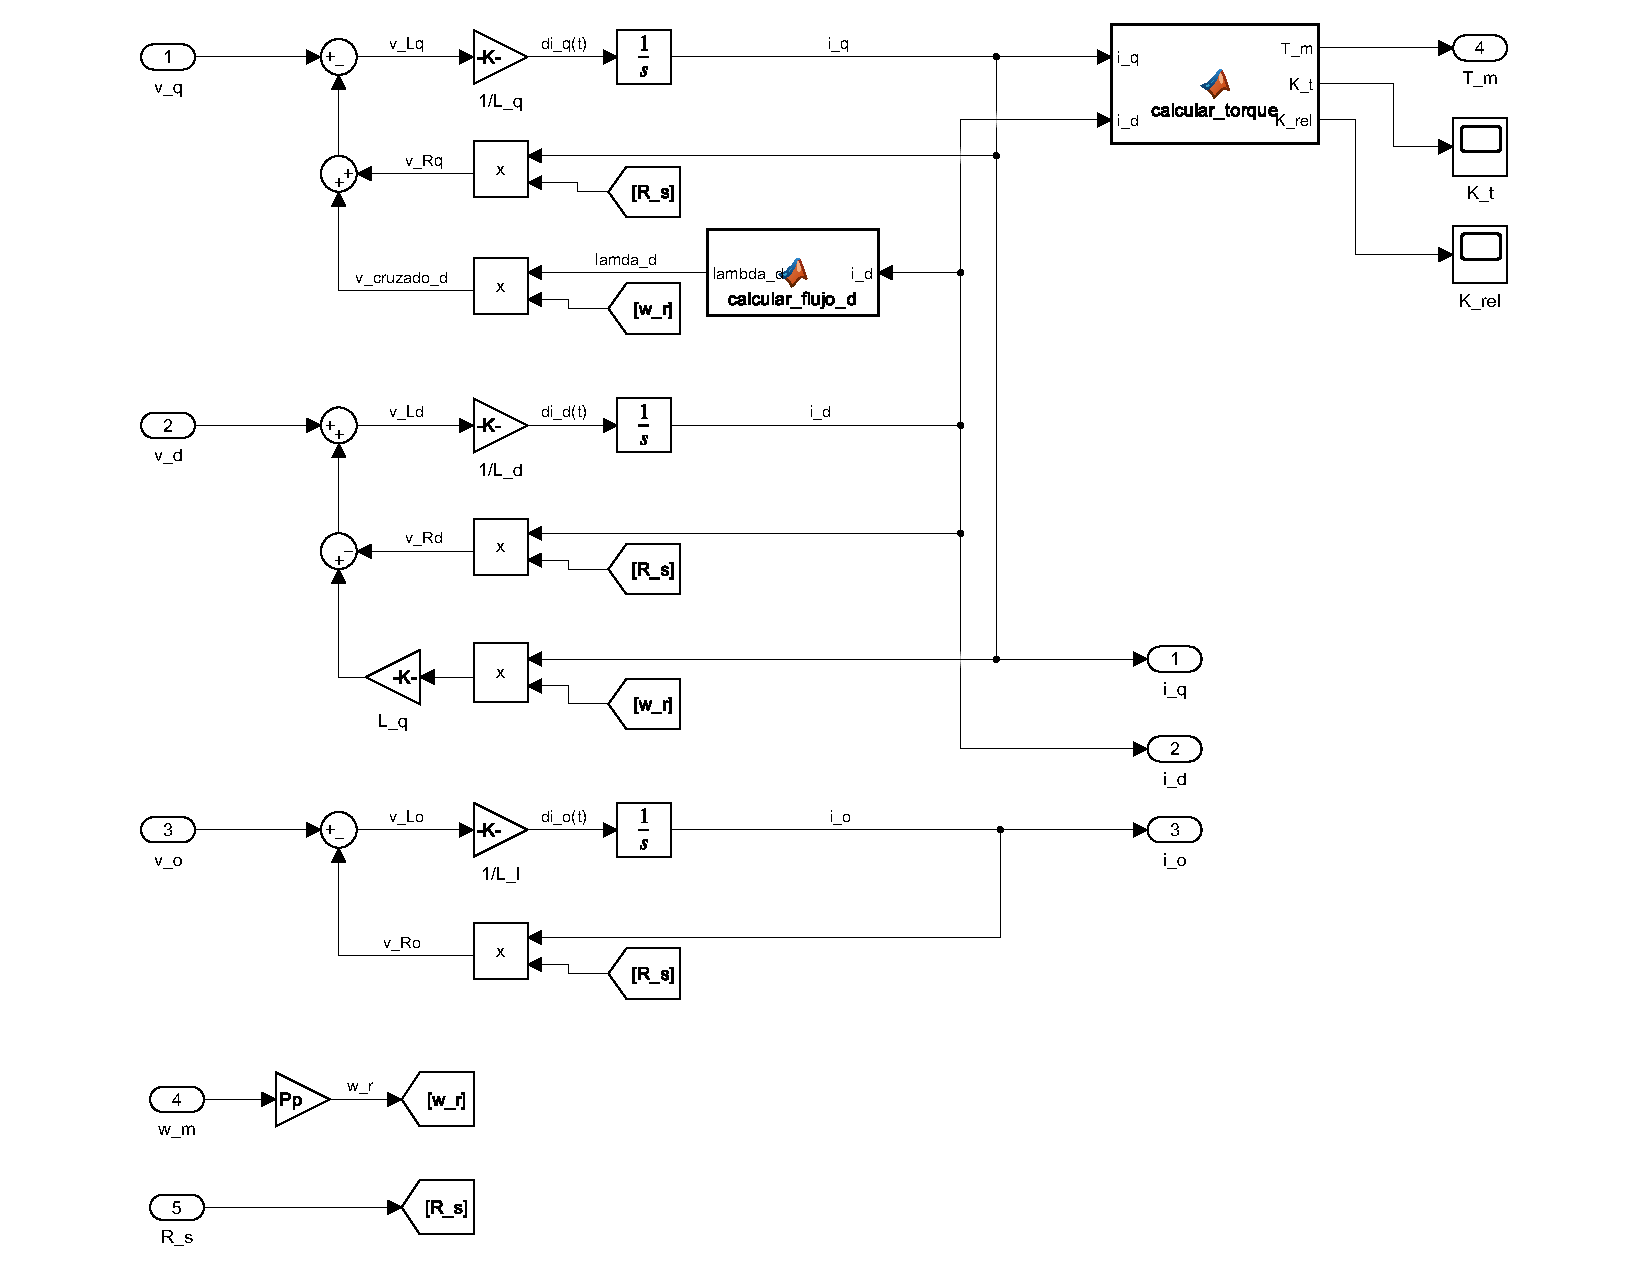
\includegraphics[width=0.95\textwidth]{img/subsistema_electromagnetico.pdf}
	\caption{Diagrama de bloques del subsistema electromagnético de la PMSM en coordenadas $qd0$, con acceso físico mediante tensiones y corrientes trifásicas $abc$.}
	\label{fig:diagrama_electromecanico_equivalente}
\end{figure}


\paragraph{Resistencia de estator dependiente de la temperatura.}
Las pérdidas por efecto Joule elevan la temperatura del bobinado $T_s^{\circ}(t)$, lo cual incrementa la resistencia de fase del estator. Este comportamiento se modela como:

\begin{equation}
	R_s\left(T_s^{\circ}(t)\right)=R_{sREF}\left[1+\alpha_{Cu}\left(T_s^{\circ}(t)-T_{sREF}^{\circ}\right)\right],
	\label{eq:resistencia_termica}
\end{equation}

donde $R_{sREF}$ es la resistencia medida a la temperatura de referencia $T_{sREF}^{\circ}$ y $\alpha_{Cu}$ es el coeficiente de temperatura del cobre. En el diagrama en coordenadas $qd0$, esta resistencia variable se calcula a partir de la temperatura obtenida por el balance térmico escrito en las mismas coordenadas, de modo que la retroalimentación térmica se expresa como:

\begin{equation*}
	\left(i_{qs}^{r},i_{ds}^{r},i_{0s}\right) \longrightarrow P_{s,perd}^{qd0}(t) \longrightarrow T_s^{\circ}(t) \longrightarrow R_s\left(T_s^{\circ}(t)\right).
\end{equation*}

\paragraph{Modelo térmico del estator.}
Las pérdidas eléctricas consideradas corresponden únicamente a la disipación resistiva por efecto Joule. En coordenadas reales de fase, la potencia total disipada es:

\begin{equation}
	P_{s,perd}^{abc}(t)=R_s\left(T_s^{\circ}(t)\right)\left[i_{as}^{2}(t)+i_{bs}^{2}(t)+i_{cs}^{2}(t)\right].
	\label{eq:potencia_joule_abc}
\end{equation}

Debido a la forma invariante en amplitud de la transformación de Park utilizada, se cumple la relación:

\begin{equation*}
	i_{as}^{2}(t)+i_{bs}^{2}(t)+i_{cs}^{2}(t)
	=\frac{3}{2}\left[\left(i_{qs}^{r}(t)\right)^2+\left(i_{ds}^{r}(t)\right)^2+2\left(i_{0s}(t)\right)^2\right].
\end{equation*}

Por lo tanto, la misma potencia de pérdidas puede expresarse de manera equivalente en coordenadas virtuales $qd0$ como:

\begin{equation}
	P_{s,perd}^{qd0}(t)=\frac{3}{2}R_s\left(T_s^{\circ}(t)\right)
	\left[\left(i_{qs}^{r}(t)\right)^2+\left(i_{ds}^{r}(t)\right)^2+2\left(i_{0s}(t)\right)^2\right].
	\label{eq:potencia_joule_qd0}
\end{equation}

Esta última forma es la más conveniente para el diagrama implementado en coordenadas $qd0$, ya que utiliza directamente las corrientes internas del subsistema eléctrico. Si luego se impone la condición particular de sistema equilibrado con neutro flotante, $i_{0s}(t)\equiv 0$, la expresión se reduce a:

\begin{equation*}
	P_{s,perd}^{qd0}(t)=\frac{3}{2}R_s\left(T_s^{\circ}(t)\right)
	\left[\left(i_{qs}^{r}(t)\right)^2+\left(i_{ds}^{r}(t)\right)^2\right].
\end{equation*}

Considerando el balance de energía entre el calor generado y el calor disipado hacia el ambiente a través de la resistencia térmica $R_{ts-amb}$, la dinámica de la temperatura del estator queda:

\begin{equation}
	\frac{dT_s^{\circ}}{dt}=\frac{1}{C_{ts}}\left[\frac{3}{2}R_s\left(T_s^{\circ}\right)\left(\left(i_{qs}^{r}\right)^2+\left(i_{ds}^{r}\right)^2+2i_{0s}^{2}\right)-\frac{T_s^{\circ}-T_{amb}^{\circ}}{R_{ts-amb}}\right].
	\label{eq:dinamica_termica_estator}
\end{equation}

\paragraph{Diagrama de bloques del subsistema térmico.}
La Fig.~\ref{fig:diagrama_termico_equivalente} muestra la implementación del modelo térmico. En esta versión, el cálculo de potencia se representa directamente en coordenadas $qd0$, tomando como entradas $i_{qs}^{r}$, $i_{ds}^{r}$ e $i_{0s}$. A partir de dichas corrientes se obtiene $P_{s,perd}^{qd0}(t)$, luego se integra la ecuación diferencial térmica y finalmente se retroalimenta $R_s(T_s^{\circ})$ al subsistema eléctrico.

\begin{figure}[H]
	\centering
	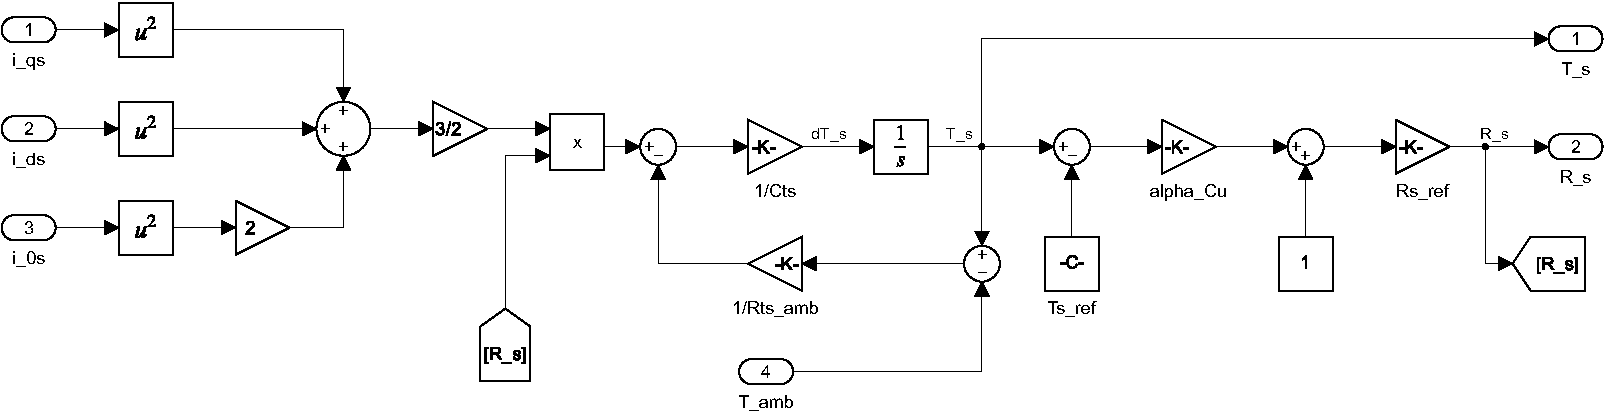
\includegraphics[width=0.95\textwidth]{img/subsistema_termico.pdf}
	\caption{Diagrama de bloques del subsistema térmico en coordenadas $qd0$, con cálculo de pérdidas Joule, dinámica de temperatura y retroalimentación de $R_s(T_s^{\circ})$.}
	\label{fig:diagrama_termico_equivalente}
\end{figure}

\paragraph{Variables de estado, entradas y salidas.}
Para sistematizar el modelo general, se adopta el siguiente vector de estado global de sexto orden:

\begin{equation}
	x(t)=
	\begin{bmatrix}
		x_1(t)\\
		x_2(t)\\
		x_3(t)\\
		x_4(t)\\
		x_5(t)\\
		x_6(t)
	\end{bmatrix}
	=
	\begin{bmatrix}
		\theta_m(t)\\
		\omega_m(t)\\
		i_{qs}^{r}(t)\\
		i_{ds}^{r}(t)\\
		i_{0s}(t)\\
		T_s^{\circ}(t)
	\end{bmatrix},
	\qquad
	x(t_0)=x_0.
	\label{eq:estado_global_p2}
\end{equation}

Las entradas externas del modelo se separan en entradas de control, manipulables por el inversor, y entradas de perturbación exógenas:

\begin{equation*}
	u_c(t)=\begin{bmatrix}v_{qs}^{r}(t)\\v_{ds}^{r}(t)\\v_{0s}(t)\end{bmatrix},
	\qquad
	u_d(t)=\begin{bmatrix}T_{ld}(t)\\T_{amb}^{\circ}(t)\end{bmatrix}.
\end{equation*}

Para expresar el modelo en forma compacta, se define el vector de entrada aumentado:

\begin{equation}
	u(t)=
	\begin{bmatrix}
		v_{qs}^{r}(t)\\
		v_{ds}^{r}(t)\\
		v_{0s}(t)\\
		T_{ld}(t)\\
		T_{amb}^{\circ}(t)
	\end{bmatrix}
	=
	\begin{bmatrix}
		u_1(t)\\
		u_2(t)\\
		u_3(t)\\
		u_4(t)\\
		u_5(t)
	\end{bmatrix}.
	\label{eq:entradas_global_p2}
\end{equation}

La salida principal de interés para el control de movimiento es la posición angular de la carga:

\begin{equation*}
	y_p(t)=q(t)=\frac{\theta_m(t)}{r}=\frac{x_1(t)}{r}.
\end{equation*}

Por lo tanto, la matriz de salida asociada a la variable controlada es:

\begin{equation*}
	C_p=\begin{bmatrix}\frac{1}{r} & 0 & 0 & 0 & 0 & 0\end{bmatrix}.
\end{equation*}

A su vez, el sensor de posición se encuentra montado sobre el eje del motor, por lo que la salida medida disponible para la retroalimentación es:

\begin{equation*}
	y_s(t)=\theta_m(t)=x_1(t),
	\qquad
	C_s=\begin{bmatrix}1 & 0 & 0 & 0 & 0 & 0\end{bmatrix}.
\end{equation*}

Las corrientes físicas de fase se obtienen como salida adicional mediante la transformación inversa de Park:

\begin{equation*}
	\begin{bmatrix}
		i_{as}(t)\\
		i_{bs}(t)\\
		i_{cs}(t)
	\end{bmatrix}
	=
	\mathbf{T}_{P}^{-1}\left(\theta_r(t)\right)
	\begin{bmatrix}
		x_3(t)\\
		x_4(t)\\
		x_5(t)
	\end{bmatrix}.
\end{equation*}

\paragraph{Modelo global no lineal en espacio de estados.}
Agrupando las ecuaciones diferenciales mecánicas \eqref{eq:omega_global_acoplada}, eléctricas \eqref{eq:dinamica_corrientes_qd0} y térmicas \eqref{eq:dinamica_termica_estator}, el modelo global no lineal acoplado queda:

\begin{equation}
	\boxed{
		\begin{aligned}
			\dot{x}_1 &= x_2,\\[1mm]
			\dot{x}_2 &= \frac{1}{J_{eq}}\left[K_t x_3+K_{rel}x_4x_3-b_{eq}x_2-\frac{gk_l}{r}\sin\left(\frac{x_1}{r}\right)-\frac{u_4}{r}\right],\\[1mm]
			\dot{x}_3 &= \frac{1}{L_q}\left[u_1-R_s(x_6)x_3-\left(\lambda_m^{\prime r}+L_d x_4\right)P_p x_2\right],\\[1mm]
			\dot{x}_4 &= \frac{1}{L_d}\left[u_2-R_s(x_6)x_4+L_q x_3 P_p x_2\right],\\[1mm]
			\dot{x}_5 &= \frac{1}{L_{ls}}\left[u_3-R_s(x_6)x_5\right],\\[1mm]
			\dot{x}_6 &= \frac{1}{C_{ts}}\left[\frac{3}{2}R_s(x_6)\left(x_3^2+x_4^2+2x_5^2\right)-\frac{x_6-u_5}{R_{ts-amb}}\right],\\[2mm]
			y_p &= \frac{x_1}{r}.
		\end{aligned}
	}
	\label{eq:modelo_global_nl}
\end{equation}

El modelo \eqref{eq:modelo_global_nl} es fuertemente no lineal debido a múltiples factores estructurales: el acoplamiento cruzado de corrientes que genera el torque de reluctancia ($x_4x_3$), las fuerzas contraelectromotrices inducidas que mezclan velocidad y corrientes ($x_4x_2$ y $x_3x_2$), la dependencia paramétrica de la resistencia con el estado térmico ($R_s(x_6)$), los términos cuadráticos de inyección de potencia calorífica ($x_3^2$, $x_4^2$, $x_5^2$) y el torque gravitacional no lineal ($\sin(x_1/r)$).

Si se impone la condición física particular de sistema trifásico equilibrado con neutro flotante, entonces $x_5(t)=i_{0s}(t)\equiv 0$ y $u_3(t)=v_{0s}(t)\equiv 0$. En ese caso, la quinta ecuación se desacopla y el modelo se reduce al caso de quinto orden utilizado habitualmente para el análisis de la PMSM balanceada.

\paragraph{Modelo Global NL de la planta.}
La Figura~\ref{fig:modelo_global_nl} muestra la implementación en Simulink del modelo global no lineal del sistema completo. En el esquema deben observarse los principales subsistemas del accionamiento: generador o referencia trifásica, inversor idealizado, transformación de Park directa $abc\rightarrow qd0$, subsistema eléctrico de la PMSM, subsistema mecánico equivalente, transformación inversa de Park $qd0\rightarrow abc$ y subsistema térmico del estator con retroalimentación de $R_s(T_s^{\circ})$.

\begin{figure}[H]
	\centering
	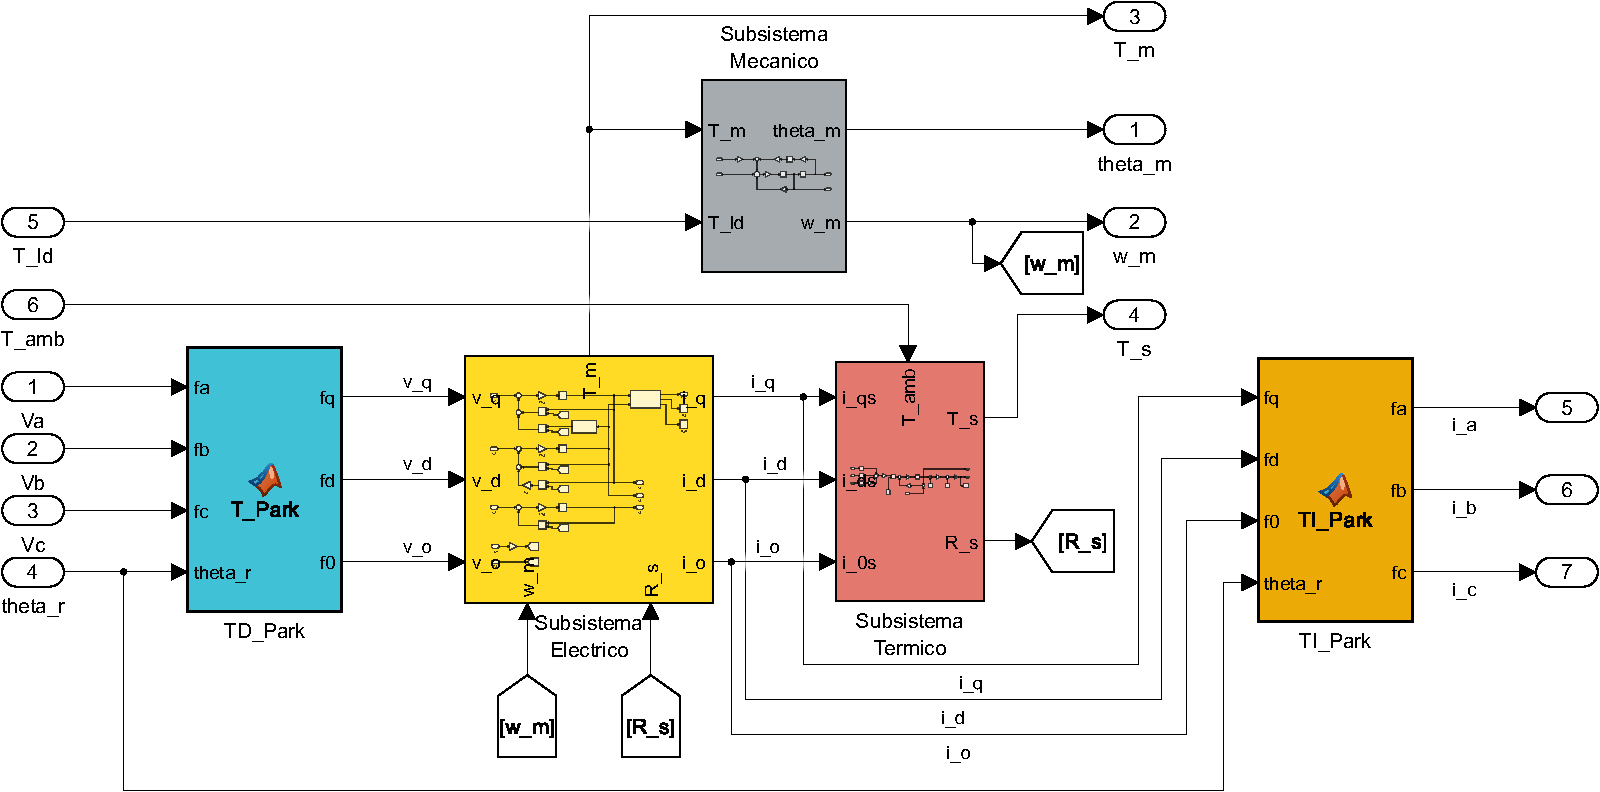
\includegraphics[width=\textwidth]{img/modelo_global_nl.pdf}
	\caption{Modelo global no lineal del accionamiento PMSM implementado en Simulink. El diagrama integra las transformaciones de Park directa e inversa, el subsistema eléctrico en coordenadas $qd0$, el subsistema mecánico equivalente, el cálculo térmico de pérdidas Joule y la retroalimentación de la resistencia estatórica variable $R_s(T_s^{\circ})$.}
	\label{fig:modelo_global_nl}
\end{figure}


% ---------------------------------------------------------
\subsubsection{Linealización Jacobiana: Modelo global LPV}

\paragraph{Objetivo de la linealización.}

El modelo global no lineal de quinto orden obtenido en \eqref{eq:modelo_global_nl} representa con alta fidelidad la dinámica de la planta física completa. 
Sin embargo, su fuerte acoplamiento y naturaleza no lineal impiden la aplicación directa de las herramientas clásicas de análisis y síntesis de control 
(como el lugar de las raíces, diagramas de Bode o ubicación de polos), las cuales asumen sistemas Lineales e Invariantes en el Tiempo (LTI).

Para sortear este obstáculo, se realiza una linealización Jacobiana basada en la expansión en serie de Taylor alrededor de un punto genérico de operación. 
Debido a que las matrices dinámicas resultantes dependerán de las coordenadas exactas de dicho punto (como la posición espacial del péndulo, la velocidad o la temperatura), 
el resultado es un modelo lineal local con parámetros variables, conocido en la literatura de control como modelo LPV (\textit{Linear Parameter Varying}).

\paragraph{Pequeñas variaciones alrededor de un punto de operación.}

Dado el sistema no lineal en espacio de estados $\dot{x}(t) = f(x(t),u(t))$ y $y(t) = g(x(t),u(t))$, se define un punto genérico de operación nominal dado por los vectores constantes de estado y de entrada:

\begin{equation*}
    x^o = \begin{bmatrix}
        \theta_m^o & \omega_m^o & I_q^o & I_d^o & T_s^o
    \end{bmatrix}^{T},
    \qquad
    u^o = \begin{bmatrix}
        V_q^o & V_d^o & T_{ld}^o & T_{amb}^o
    \end{bmatrix}^{T}.
\end{equation*}

Se asume que el sistema experimenta pequeñas perturbaciones o variaciones dinámicas $(\Delta)$ respecto a esta condición nominal, tal que:

\begin{equation*}
	x(t)=x^o+\Delta x(t),
	\qquad
	u(t)=u^o+\Delta u(t).
\end{equation*}

Aplicando una aproximación por serie de Taylor truncada a primer orden, la dinámica local de las pequeñas variaciones queda descrita por el sistema linealizado:

\begin{equation}
    \begin{aligned}
        \Delta\dot{x}(t) &= A(x^o,u^o)\Delta x(t) + B(x^o,u^o)\Delta u(t), \\
        \Delta y_p(t) &= C(x^o,u^o)\Delta x(t) + D(x^o,u^o)\Delta u(t).
    \end{aligned}
    \label{eq:lpv_sistema}
\end{equation}

Las matrices Jacobianas del sistema se evalúan estrictamente en el punto de operación, determinándose componente a componente como:

\begin{equation*}
    A_{ij} = \left. \frac{\partial f_i}{\partial x_j} \right|_{x^o,u^o}, \qquad 
    B_{ij} = \left. \frac{\partial f_i}{\partial u_j} \right|_{x^o,u^o}, \qquad
    C_{ij} = \left. \frac{\partial g_i}{\partial x_j} \right|_{x^o,u^o}, \qquad
    D_{ij} = \left. \frac{\partial g_i}{\partial u_j} \right|_{x^o,u^o}.
\end{equation*}

\paragraph{Espacio de operación global no lineal cuasi-estacionario.}

Para que el punto de evaluación $(x^o, u^o)$ sea matemáticamente válido, debe pertenecer al espacio de soluciones de equilibrio del sistema no lineal; 
es decir, anular las derivadas de los estados lentos o, en el caso de accionamientos eléctricos, establecer un régimen permanente en el marco rotórico.

Igualando a cero las derivadas de la velocidad, las corrientes y la temperatura del modelo \eqref{eq:modelo_global_nl}, 
se obtienen las ecuaciones algebraicas que restringen el punto de operación cuasi-estacionario:

\begin{equation}
    \begin{aligned}
        0 &= K_t I_q^o + K_{rel}I_d^o I_q^o - b_{eq}\omega_m^o - \frac{gk_l}{r}\sin\left(\frac{\theta_m^o}{r}\right) - \frac{T_{ld}^o}{r},\\[1mm]
        0 &= V_q^o - R_s(T_s^o) I_q^o - \left(\lambda_m^{\prime r}+L_d I_d^o\right)P_p\omega_m^o,\\[1mm]
        0 &= V_d^o - R_s(T_s^o) I_d^o + L_q I_q^o P_p\omega_m^o,\\[1mm]
        0 &= \frac{3}{2}R_s(T_s^o)\left[(I_q^o)^2+(I_d^o)^2\right] - \frac{T_s^o-T_{amb}^o}{R_{ts-amb}}.
    \end{aligned}
    \label{eq:condiciones_equilibrio}
\end{equation}

La Ecuación \eqref{eq:condiciones_equilibrio} permite hallar los requerimientos de tensión y corriente en estado estacionario para sostener cualquier consigna mecánica. 
Para un equilibrio estricto de posición (por ejemplo, mantener el brazo robótico frenado en un ángulo específico contra la gravedad), se debe cumplir adicionalmente $\omega_m^o = 0$. 
En contraste, si el objetivo es analizar el seguimiento a velocidad constante, se establece $\omega_m^o \neq 0$ y el punto se interpreta como un estado cuasi-estacionario o "congelado". 
Es crucial notar que, dado el uso del marco $qd0$, una velocidad mecánica constante se traduce efectivamente en variables de estado constantes para las corrientes, 
haciendo matemáticamente factible la linealización Jacobiana.

\paragraph{Matriz de Estado $A(x^o,u^o)$ del modelo LPV.}

Para evaluar las derivadas parciales que involucran a la resistencia térmica, 
resulta conveniente definir la constante de variación de resistencia con la temperatura:

\begin{equation}
	\kappa_R=\frac{dR_s}{dT_s^{\circ}}=R_{sREF}\alpha_{Cu},
\end{equation}

Calculando el Jacobiano del sistema \eqref{eq:modelo_global_nl} respecto al vector de estado, 
la matriz de estado local queda definida por:

\begin{equation}
	A(x^o,u^o)=
	\begin{bmatrix}
		0 & 1 & 0 & 0 & 0\\[1mm]
		A_{21} & A_{22} & A_{23} & A_{24} & 0\\[1mm]
		0 & A_{32} & A_{33} & A_{34} & A_{35}\\[1mm]
		0 & A_{42} & A_{43} & A_{44} & A_{45}\\[1mm]
		0 & 0 & A_{53} & A_{54} & A_{55}
	\end{bmatrix},
	\label{eq:matriz_a_lpv}
\end{equation}

cuyos coeficientes no nulos, evaluados en el punto de operación, se agrupan según su naturaleza dinámica:

\begin{equation*}
    \begin{aligned}
        & \text{Mecánicos:} &
        A_{21} &= -\frac{g k_l}{J_{eq}r^2}\cos\left(\frac{\theta_m^o}{r}\right), \quad &
        A_{22} &= -\frac{b_{eq}}{J_{eq}}, \\
        & &
        A_{23} &= \frac{K_t+K_{rel}I_d^o}{J_{eq}}, \quad &
        A_{24} &= \frac{K_{rel}I_q^o}{J_{eq}}. \\[2mm]
        & \text{Eléctricos ($q$):} &
        A_{32} &= -\frac{P_p\left(\lambda_m^{\prime r}+L_d I_d^o\right)}{L_q}, \quad &
        A_{33} &= -\frac{R_s^o}{L_q}, \\
        & &
        A_{34} &= -\frac{L_d P_p\omega_m^o}{L_q}, \quad &
        A_{35} &= -\frac{\kappa_R I_q^o}{L_q}. \\[2mm]
        & \text{Eléctricos ($d$):} &
        A_{42} &= \frac{L_q P_p I_q^o}{L_d}, \quad &
        A_{43} &= \frac{L_q P_p \omega_m^o}{L_d}, \\
        & &
        A_{44} &= -\frac{R_s^o}{L_d}, \quad &
        A_{45} &= -\frac{\kappa_R I_d^o}{L_d}. \\[2mm]
        & \text{Térmicos:} &
        A_{53} &= \frac{3 R_s^o I_q^o}{C_{ts}}, \quad &
        A_{54} &= \frac{3 R_s^o I_d^o}{C_{ts}}, \\
        & &
        A_{55} &= \frac{1}{C_{ts}} \left[ \frac{3}{2}\kappa_R\left((I_q^o)^2+(I_d^o)^2\right) -\frac{1}{R_{ts-amb}} \right].
    \end{aligned}
\end{equation*}

\paragraph{Matriz de Entrada $B(x^o,u^o)$ y Salida $C$.}

Derivando el sistema \eqref{eq:modelo_global_nl} respecto al vector de entradas aumentado $u = \begin{bmatrix} v_{qs}^r & v_{ds}^r & T_{ld} & T_{amb}^\circ \end{bmatrix}^T$, 
se obtiene la matriz Jacobiana de entrada:

\begin{equation}
	B(x^o,u^o)=
	\begin{bmatrix}
		0 & 0 & 0 & 0\\[1mm]
		0 & 0 & -\dfrac{1}{J_{eq}r} & 0\\[3mm]
		\dfrac{1}{L_q} & 0 & 0 & 0\\[3mm]
		0 & \dfrac{1}{L_d} & 0 & 0\\[3mm]
		0 & 0 & 0 & \dfrac{1}{C_{ts}R_{ts-amb}}
	\end{bmatrix}.
	\label{eq:matriz_b_lpv}
\end{equation}

Finalmente, la ecuación de salida para la variable controlada $y_p(t) = q(t) = \theta_m(t)/r$ es lineal, 
por lo que sus matrices asociadas resultan invariantes respecto al punto de operación:

\begin{equation}
    C_p = \begin{bmatrix} \dfrac{1}{r} & 0 & 0 & 0 & 0 \end{bmatrix}, \qquad D = \begin{bmatrix} 0 & 0 & 0 & 0 \end{bmatrix}.
    \label{eq:matrices_cd_lpv}
\end{equation}

\paragraph{Conclusión del modelo LPV.}

Como queda en evidencia en el cálculo analítico, el modelo es de tipo \textit{Linear Parameter Varying} (LPV) ya que los autovalores 
y la dinámica de las matrices locales $A(x^o,u^o)$ dependen fuertemente del punto de evaluación: 
la posición angular espacial $\theta_m^o$ (modificando la rigidez gravitacional en $A_{21}$), 
la velocidad de régimen $\omega_m^o$, las corrientes de carga $I_q^o, I_d^o$, 
y el estado térmico de la resistencia del bobinado $R_s^o(T_s^o)$.

% ---------------------------------------------------------
\subsubsection{Linealización por retroalimentación NO LINEAL y modelo LTI equivalente}

La linealización exacta por retroalimentación no lineal utiliza la capacidad de cálculo del controlador para cancelar activamente los acoplamientos y no linealidades internas de la máquina. 
El resultado es una planta equivalente artificialmente simplificada, ideal para el diseño de lazos de control lineales.


% ---------------------------------------------------------
\paragraph{I) Ecuaciones vectoriales/matriciales LTI de estado.}

Para obtener el modelo LTI equivalente se parte del modelo global no lineal desarrollado previamente, aplicando las hipótesis propias del control vectorial con campo orientado. El objetivo de este inciso es obtener un modelo electromecánico reducido de tres estados, útil para el análisis a lazo abierto, la construcción del diagrama de bloques, las funciones de transferencia y los análisis posteriores de estabilidad, controlabilidad y observabilidad.

La condición fundamental impuesta es:

\begin{equation*}
	i_{ds}^r(t) \equiv 0.
\end{equation*}

Bajo esta condición, el término de reluctancia del torque electromagnético se anula, ya que depende del producto $i_{ds}^r(t)i_{qs}^r(t)$. Por lo tanto, el torque queda determinado únicamente por la corriente del eje $q$:

\begin{equation*}
	T_m(t)
	=
	\frac{3}{2}P_p\lambda_m^{\prime r} i_{qs}^r(t).
\end{equation*}

Se define la constante de torque:

\begin{equation*}
	K_t = \frac{3}{2}P_p\lambda_m^{\prime r},
\end{equation*}

por lo que:

\begin{equation*}
	T_m(t)=K_t i_{qs}^r(t).
\end{equation*}

En la ecuación eléctrica del eje $q$, al imponer $i_{ds}^r(t)=0$, desaparece el término asociado a $L_d i_{ds}^r(t)$. Además, como $\omega_r(t)=P_p\omega_m(t)$, se define la constante equivalente de fuerza contraelectromotriz:

\begin{equation*}
	K_E=P_p\lambda_m^{\prime r}.
\end{equation*}

Respecto del subsistema térmico, no se lo elimina físicamente del modelo, sino que se evita su acoplamiento no lineal con el subsistema eléctrico dentro del modelo LTI de diseño. En el modelo no lineal completo, la resistencia estatórica depende de la temperatura del bobinado. Si dicha dependencia se conserva dentro de la ecuación eléctrica, aparece un acoplamiento térmico-eléctrico, ya que $R_s(T_s)$ multiplica a las corrientes del estator.

Para obtener el modelo LTI equivalente, se adopta una resistencia estatórica constante evaluada en un punto de referencia u operación:

\begin{equation*}
	R_s(T_s)\approx R_{s0}=R_s(T_{s0}).
\end{equation*}

En particular, puede tomarse $R_{s0}$ como la resistencia nominal correspondiente a una temperatura de referencia:

\begin{equation*}
	R_{s0}=R_s(T_{s,ref}),
\end{equation*}

o bien como la resistencia correspondiente a una temperatura de operación fija. Esta aproximación es razonable para el modelo de diseño porque la dinámica térmica es considerablemente más lenta que la dinámica eléctrica y mecánica. Por lo tanto, durante los transitorios principales de corriente, velocidad y posición, la variación instantánea de $R_s$ puede considerarse pequeña.

Con estas consideraciones, la dinámica eléctrica del eje $q$ queda:

\begin{equation*}
	\dot{i}_{qs}^r(t)
	=
	-\frac{K_E}{L_q}\omega_m(t)
	-\frac{R_{s0}}{L_q}i_{qs}^r(t)
	+\frac{1}{L_q}v_{qs}^r(t).
\end{equation*}

Por otra parte, el torque gravitacional del modelo mecánico mantiene una dependencia no lineal con la posición angular:

\begin{equation*}
	T_{g,eq}(t)
	=
	\frac{gk_l}{r}
	\sin\left(\frac{\theta_m(t)}{r}\right).
\end{equation*}

Para obtener un modelo lineal alrededor del equilibrio estable, se aplica la aproximación de Taylor de primer orden:

\begin{equation*}
	\sin(x)\approx x,
	\qquad
	x=\frac{\theta_m(t)}{r}.
\end{equation*}

Entonces:

\begin{equation*}
	\frac{gk_l}{r}
	\sin\left(\frac{\theta_m(t)}{r}\right)
	\approx
	\frac{gk_l}{r^2}\theta_m(t).
\end{equation*}

Se define la rigidez gravitacional equivalente referida al eje del motor como:

\begin{equation*}
	K_g=\frac{gk_l}{r^2}.
\end{equation*}

Por lo tanto, el torque gravitacional linealizado queda:

\begin{equation*}
	T_{g,eq}(t)\approx K_g\theta_m(t).
\end{equation*}

Reemplazando el torque electromagnético, la fuerza contraelectromotriz y la gravedad linealizada en las ecuaciones del sistema, se obtiene el siguiente modelo LTI electromecánico de tres estados:

\begin{equation}
	\begin{aligned}
		\dot{\theta}_m(t) &= \omega_m(t),\\[1mm]
		\dot{\omega}_m(t) &=
		-\frac{K_g}{J_{eq}}\theta_m(t)
		-\frac{b_{eq}}{J_{eq}}\omega_m(t)
		+\frac{K_t}{J_{eq}}i_{qs}^r(t)
		-\frac{1}{J_{eq}r}T_{ld}(t),\\[1mm]
		\dot{i}_{qs}^r(t) &=
		-\frac{K_E}{L_q}\omega_m(t)
		-\frac{R_{s0}}{L_q}i_{qs}^r(t)
		+\frac{1}{L_q}v_{qs}^r(t).
	\end{aligned}
	\label{eq:lti_3estados_ecuaciones}
\end{equation}

El vector de estado del modelo LTI reducido se define como:

\begin{equation*}
	x_{LTI}(t)
	=
	\begin{bmatrix}
		\theta_m(t)\\
		\omega_m(t)\\
		i_{qs}^r(t)
	\end{bmatrix},
	\qquad
	x_{LTI}(t_0)
	=
	\begin{bmatrix}
		\theta_m(t_0)\\
		\omega_m(t_0)\\
		i_{qs}^r(t_0)
	\end{bmatrix}.
\end{equation*}

La entrada de control es la tensión virtual del eje $q$:

\begin{equation*}
	u_c(t)=v_{qs}^r(t),
\end{equation*}

mientras que la perturbación mecánica externa se considera como:

\begin{equation*}
	u_d(t)=T_{ld}(t).
\end{equation*}

De esta manera, el modelo LTI electromecánico puede escribirse como:

\begin{equation}
	\dot{x}_{LTI}(t)
	=
	A_{LTI}x_{LTI}(t)
	+
	B_cu_c(t)
	+
	B_du_d(t),
	\label{eq:modelo_lti_3x3_general}
\end{equation}

donde:

\begin{equation}
	A_{LTI}
	=
	\begin{bmatrix}
		0 & 1 & 0\\[2mm]
		-\dfrac{K_g}{J_{eq}} & -\dfrac{b_{eq}}{J_{eq}} & \dfrac{K_t}{J_{eq}}\\[3mm]
		0 & -\dfrac{K_E}{L_q} & -\dfrac{R_{s0}}{L_q}
	\end{bmatrix},
	\qquad
	B_c
	=
	\begin{bmatrix}
		0\\[2mm]
		0\\[2mm]
		\dfrac{1}{L_q}
	\end{bmatrix},
	\qquad
	B_d
	=
	\begin{bmatrix}
		0\\[2mm]
		-\dfrac{1}{J_{eq}r}\\[2mm]
		0
	\end{bmatrix}.
	\label{eq:matrices_lti_3x3}
\end{equation}

Si se define directamente el torque de perturbación equivalente referido al eje del motor como:

\begin{equation*}
	T_{ld,eq}(t)=\frac{T_{ld}(t)}{r},
\end{equation*}

entonces la matriz de perturbación puede escribirse alternativamente como:

\begin{equation*}
	B_{d,eq}
	=
	\begin{bmatrix}
		0\\[2mm]
		-\dfrac{1}{J_{eq}}\\[2mm]
		0
	\end{bmatrix}.
\end{equation*}

La salida física de interés para el control de posición de la articulación es:

\begin{equation*}
	q(t)=\frac{\theta_m(t)}{r}.
\end{equation*}

Por lo tanto, si la salida del modelo se toma como la posición angular de la carga:

\begin{equation*}
	y_p(t)=q(t)=C_p x_{LTI}(t),
	\qquad
	C_p=
	\begin{bmatrix}
		\dfrac{1}{r} & 0 & 0
	\end{bmatrix}.
\end{equation*}

Si, en cambio, se considera como salida medida la posición del eje del motor, por ejemplo mediante encoder, se tiene:

\begin{equation*}
	y_s(t)=\theta_m(t)=C_s x_{LTI}(t),
	\qquad
	C_s=
	\begin{bmatrix}
		1 & 0 & 0
	\end{bmatrix}.
\end{equation*}

En ambos casos:

\begin{equation*}
	D=0.
\end{equation*}

El modelo anterior constituye el sistema LTI principal de orden tres. En él se conservan las dinámicas de posición, velocidad y corriente de eje $q$, mientras que la corriente de eje directo $i_{ds}^r(t)$ no se incluye como estado porque se impone la condición de campo orientado $i_{ds}^r(t)\equiv 0$. La dinámica residual asociada al eje directo se analiza posteriormente al estudiar la ley mínima de control.

\medskip

\noindent\textbf{Dinámica térmica auxiliar desacoplada.}

La dinámica térmica del estator se conserva separada del modelo LTI electromecánico de tres estados. Para ello se parte del balance térmico:

\begin{equation*}
	P_{s,\mathrm{perd}}(t)
	=
	C_{ts}\dot{T}_s(t)
	+
	\frac{T_s(t)-T_{amb}(t)}{R_{ts-amb}}.
\end{equation*}

Despejando la derivada de la temperatura:

\begin{equation}
	\dot{T}_s(t)
	=
	-\frac{1}{C_{ts}R_{ts-amb}}T_s(t)
	+\frac{1}{C_{ts}}P_{s,\mathrm{perd}}(t)
	+\frac{1}{C_{ts}R_{ts-amb}}T_{amb}(t).
	\label{eq:termica_lineal_psperd}
\end{equation}

Esta ecuación puede representarse como un subsistema lineal de primer orden, tomando como estado térmico:

\begin{equation*}
	x_T(t)=T_s(t),
\end{equation*}

y como entradas térmicas:

\begin{equation*}
	u_T(t)=
	\begin{bmatrix}
		P_{s,\mathrm{perd}}(t)\\
		T_{amb}(t)
	\end{bmatrix}.
\end{equation*}

Entonces:

\begin{equation}
	\dot{x}_T(t)
	=
	A_Tx_T(t)+B_Tu_T(t),
	\label{eq:termica_lineal_estado}
\end{equation}

con:

\begin{equation*}
	A_T
	=
	\begin{bmatrix}
		-\dfrac{1}{C_{ts}R_{ts-amb}}
	\end{bmatrix},
	\qquad
	B_T
	=
	\begin{bmatrix}
		\dfrac{1}{C_{ts}} &
		\dfrac{1}{C_{ts}R_{ts-amb}}
	\end{bmatrix}.
\end{equation*}

En esta formulación, $P_{s,\mathrm{perd}}(t)$ se considera una entrada térmica equivalente. No se incorpora dentro del modelo LTI principal la expresión no lineal completa de las pérdidas, ya que si se reemplazara directamente:

\begin{equation*}
	P_{s,\mathrm{perd}}(t)
	=
	\frac{3}{2}R_{s0}\left(i_{qs}^{r}(t)\right)^2,
\end{equation*}

la relación entre la corriente de eje $q$ y la temperatura volvería a contener una no linealidad algebraica. En la simulación, dicha potencia de pérdidas puede calcularse externamente a partir de $i_{qs}^{r}(t)$, a partir de las corrientes reales de fase medidas, o mediante un valor equivalente representativo del régimen de operación. Lo importante es que $T_s(t)$ no se realimenta sobre $R_s$ dentro de la dinámica eléctrica del modelo LTI reducido.

Por lo tanto, el sistema utilizado para los análisis de estabilidad, controlabilidad, observabilidad y funciones de transferencia es el modelo electromecánico LTI de tres estados dado por las matrices $A_{LTI}$, $B_c$ y $B_d$. La dinámica térmica queda como subsistema auxiliar desacoplado, útil para monitorear la temperatura del estator sin modificar la matriz de estado del modelo principal.
% ---------------------------------------------------------
\paragraph{II) Diagrama de bloques de estado.}

A partir de las ecuaciones obtenidas en el inciso anterior, se implementa en Simulink el diagrama de bloques del modelo LTI equivalente por realimentación no lineal. La rama principal corresponde al modelo electromecánico reducido de tres estados, cuyas variables son la posición angular del rotor $\theta_m(t)$, la velocidad angular $\omega_m(t)$ y la corriente de eje $q$, $i_{qs}^{r}(t)$.

En el mismo diagrama se incluye la perturbación mecánica externa $T_{ld}(t)$, el efecto gravitacional linealizado mediante la constante $K_g$ y una rama térmica auxiliar. Esta última recibe como entrada la potencia de pérdidas $P_{s,\mathrm{perd}}(t)$ y permite estimar la evolución de la temperatura del estator $T_s(t)$, sin realimentar dicha temperatura sobre la resistencia estatórica del modelo eléctrico. Por lo tanto, el sistema utilizado para análisis de estabilidad, controlabilidad, observabilidad y funciones de transferencia sigue siendo el modelo LTI electromecánico de orden tres.

\begin{figure}[H]
	\centering
	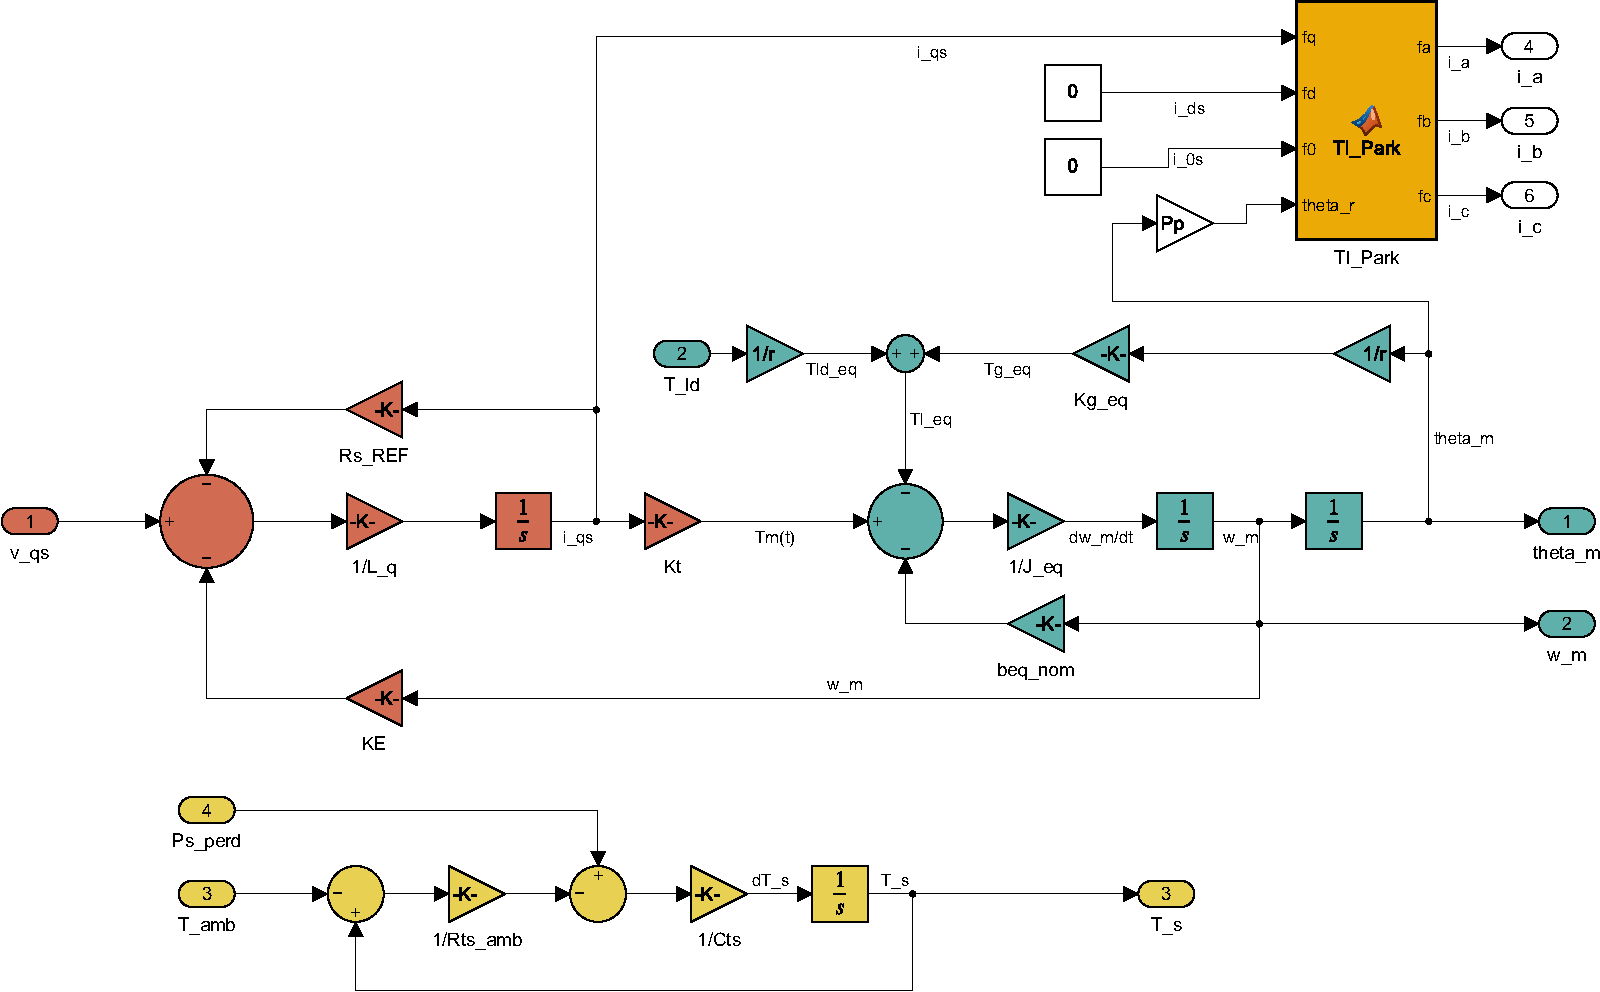
\includegraphics[width=0.95\textwidth]{img/modelo_lti_3x3.pdf}
	\caption{Diagrama de bloques del modelo LTI electromecánico equivalente por realimentación no lineal. Se muestra la dinámica principal de tres estados $v_{qs}^r(t)\rightarrow i_{qs}^r(t)\rightarrow T_m(t)\rightarrow \omega_m(t)\rightarrow \theta_m(t)$, junto con la perturbación mecánica externa, la gravedad linealizada y la rama térmica auxiliar excitada por $P_{s,\mathrm{perd}}(t)$.}
	\label{fig:sistema_lti_realimentacion_nl}
\end{figure}

% ---------------------------------------------------------
\paragraph{III) Ley de control mínima para imponer $i_{ds}^{r}(t)\equiv 0$.}

Para obtener el modelo LTI equivalente se impone la condición de campo orientado $i_{ds}^{r}(t)\equiv0$. Esta condición permite anular la corriente de eje directo, desacoplando el canal de flujo magnético del canal de torque.

Partiendo de la Ecuacion \eqref{eq:dinamica_corrientes_qd0} para la dinámica de la corriente del eje $d$:

\begin{equation}
	\frac{di_{ds}^{r}}{dt}
	=
	\frac{1}{L_d}
	\left[
	v_{ds}^r(t)
	-
	R_s i_{ds}^r(t)
	+
	L_q i_{qs}^r(t)P_p\omega_m(t)
	\right],
	\label{eq:id_para_ley_minima}
\end{equation}

se exige que:

\begin{equation*}
	i_{ds}^r(t)\equiv0,
	\qquad
	\frac{di_{ds}^{r}}{dt}\equiv0.
\end{equation*}

Al reemplazar estas condiciones en \eqref{eq:id_para_ley_minima}, queda:

\begin{equation*}
	0=
	\frac{1}{L_d}
	\left[
	v_{ds}^r(t)+L_q i_{qs}^r(t)P_p\omega_m(t)
	\right].
\end{equation*}

Por lo tanto, la ley de control mínima que debe aplicarse sobre la tensión virtual del eje directo es:

\begin{equation}
	\boxed{
		v_{ds}^{r*}(t)
		=
		-L_q i_{qs}^{r}(t)P_p\omega_m(t)
		=
		-L_q i_{qs}^{r}(t)\omega_r(t)
	}
	\label{eq:ley_minima_vd}
\end{equation}

donde $\omega_r(t)=P_p\omega_m(t)$. Esta acción cancela el acoplamiento cruzado $L_q i_{qs}^r(t)P_p\omega_m(t)$ presente en el eje $d$.

La condición inicial necesaria para que la restricción se cumpla exactamente desde el comienzo es:

\begin{equation}
	i_{ds}^r(t_0)=0.
	\label{eq:hipotesis_inicial_id}
\end{equation}

Bajo esta hipótesis, la aplicación de \eqref{eq:ley_minima_vd} mantiene $i_{ds}^r(t)=0$ para todo $t\geq t_0$. La tensión $v_{qs}^{r*}(t)$ queda libre y actúa como entrada principal del modelo LTI equivalente, mientras que para un sistema trifásico equilibrado se adopta $v_{0s}^{r*}(t)=0$.

Para llevar esta ley virtual al sistema físico, se forma el vector de tensiones de referencia en coordenadas $qd0$:

\begin{equation*}
	\mathbf{v}_{qd0s}^{r*}(t)
	=
	\begin{bmatrix}
		v_{qs}^{r*}(t)\\
		-L_q i_{qs}^{r}(t)P_p\omega_m(t)\\
		0
	\end{bmatrix},
\end{equation*}

y luego se aplica la transformación inversa de Park para obtener las referencias trifásicas $v_{as}^{*}(t)$, $v_{bs}^{*}(t)$ y $v_{cs}^{*}(t)$ que ingresan al modulador de tensión equivalente.

% -----------------------------------------------------------------
\paragraph{IV) Implementación de la ley de desacoplamiento en el modelo global no lineal.}

A partir de la ley mínima obtenida en el inciso anterior, se implementó un controlador parcial que realimenta las variables medidas necesarias y genera la tensión virtual $v_{ds}^{r*}(t)$. 
Esta acción se combina con la entrada principal $v_{qs}^{r*}(t)$ y con $v_{0s}^{r*}(t)=0$, formando el vector de tensiones en coordenadas $qd0$. Luego, mediante la transformación inversa de Park, se obtienen las tensiones trifásicas de referencia que alimentan al modulador de tensión trifásico equivalente.

El modulador se modela en esta etapa como un inversor ideal de ganancia unitaria, por lo que las referencias $v_{as}^{*}(t)$, $v_{bs}^{*}(t)$ y $v_{cs}^{*}(t)$ se aplican directamente al modelo global no lineal de la PMSM. Con esta implementación se busca comprobar que la ley mínima fuerza $i_{ds}^{r}(t)\to0$, logrando el desacoplamiento entre el canal de flujo magnético y el canal de torque. La Figura~\ref{fig:ley_control_minima} muestra el esquema implementado en Simulink.

\begin{figure}[H]
	\centering
	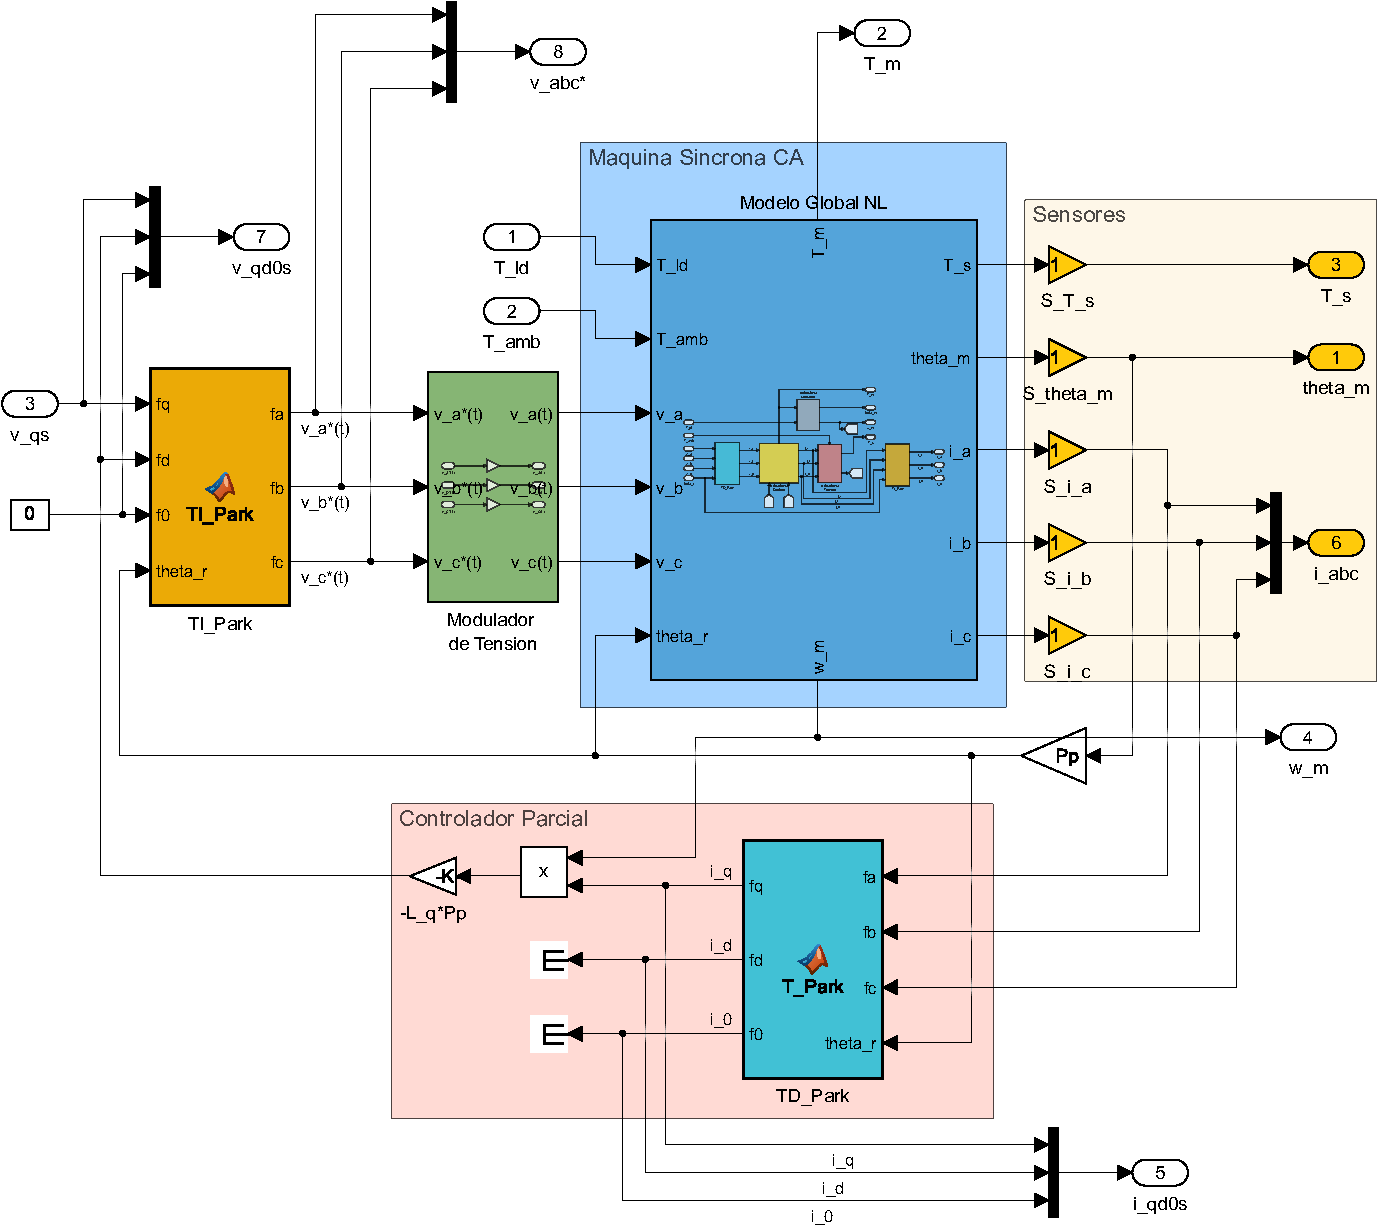
\includegraphics[width=0.95\textwidth]{img/ley_de_control_minima.pdf}
	\caption{Diagrama de bloques del sistema linealizado por realimentación parcial de estados mediante un controlador externo.}
	\label{fig:ley_control_minima}
\end{figure}

% -----------------------------------------------------------------
\paragraph{V) Dinámica residual equivalente para $i_{ds}^{r}(t)$.}
Si la condición inicial \eqref{eq:hipotesis_inicial_id} no se cumple, es decir, si:

\begin{equation*}
    i_{ds}^r(t_0) \neq 0,
\end{equation*}

la inyección de la ley mínima \eqref{eq:ley_minima_vd} conduce a una dinámica residual. Sustituyendo $v_{ds}^{r*} = -L_q i_{qs}^r P_p \omega_m$ en la ecuación diferencial de la planta para el eje $d$ \eqref{eq:id_para_ley_minima}, se obtiene:

\begin{equation*}
	\frac{di_{ds}^{r}}{dt} = \frac{-L_q i_{qs}^r P_p \omega_m - R_s i_{ds}^r + L_q i_{qs}^r P_p \omega_m}{L_d}.
\end{equation*}

Los términos de acoplamiento se cancelan exactamente y queda expuesta la dinámica libre natural del eje directo:

\begin{equation}
    \boxed{ \frac{di_{ds}^{r}}{dt} = -\frac{R_s}{L_d}i_{ds}^r. }
    \label{eq:dinamica_residual_id}
\end{equation}

La solución analítica de la Ecuación \eqref{eq:dinamica_residual_id} es un decaimiento exponencial:

\begin{equation*}
    i_{ds}^r(t) = i_{ds}^r(t_0) e^{-\frac{R_s}{L_d}(t-t_0)}.
\end{equation*}

Como $R_s > 0$ y $L_d > 0$, el polo residual:

\begin{equation*}
    p_d = -\frac{R_s}{L_d}
\end{equation*}

está siempre ubicado en el semiplano izquierdo del plano $s$. 
Por lo tanto, la corriente $i_{ds}^r$ decae exponencialmente a cero garantizando estabilidad asintótica local.

La constante de tiempo asociada a este decaimiento es:

\begin{equation*}
    \tau_d = \frac{L_d}{R_s}.
\end{equation*}

Utilizando los valores nominales de la máquina ($L_d = \SI{6.6e-3}{\henry}$ y $R_s = \SI{1.02}{\ohm}$), resulta:

\begin{equation*}
    \tau_d \approx \SI{6.47e-3}{\second}.
\end{equation*}

Por lo tanto, luego de algunos múltiplos de $\tau_d$ (escasos milisegundos), 
el valor de $i_{ds}^r$ resulta prácticamente nulo y despreciable frente a la constante de tiempo mecánica (que es órdenes de magnitud más lenta).

Este acoplamiento residual no lineal aparece temporalmente en el torque electromagnético:

\begin{equation*}
    T_m = K_t i_{qs}^r + K_{rel} i_{ds}^r i_{qs}^r.
\end{equation*}

El término residual es $T_{rel,res} = K_{rel} i_{ds}^r i_{qs}^r$. 
Este término puede despreciarse en el estudio del régimen forzado porque $i_{ds}^r(t) \rightarrow 0$ de manera exponencial sumamente rápida y porque el torque de alineación principal ($K_t i_{qs}^r$) domina casi instantáneamente el comportamiento electromecánico.

\paragraph{VI) Ley complementaria mínima en el eje $q$.}
Si bien la ley de control minima aplicada al eje $d$ logra cancelar el acoplamiento que afecta a $i_{ds}^r$, 
esta corriente no se anula de forma instantánea si su condición inicial no es nula $i_{ds}^r(t_0)=0$, sino que decae según su dinámica natural. 
Durante este transitorio, la dinámica del eje $q$ sigue afectada por un término de acoplamiento cruzado que depende de $i_{ds}^r(t)$:

\begin{equation}
	v_{qs}^{r*}(t)
	=
	L_q\frac{di_{qs}^{r}(t)}{dt}
	+R_s i_{qs}^{r}(t)
	+\lambda_m^{\prime r}P_p\omega_m(t)
	+L_d i_{ds}^{r}(t)P_p\omega_m(t).
	\label{eq:iq_con_acople}
\end{equation}

El término responsable de introducir esta no linealidad residual es:

\begin{equation*}
	L_d i_{ds}^{r}(t)P_p\omega_m(t),
\end{equation*}

debido a que contiene el producto entre dos variables dinámicas. 
En cambio, el término $\lambda_m^{\prime r}P_p\omega_m(t)$ corresponde a la fuerza contraelectromotriz de los imanes permanentes 
y es lineal respecto de $\omega_m(t)$, por lo que no requiere ser cancelarlo para obtener un modelo LTI equivalente.

Con el propósito de no introducir una nueva entrada auxiliar, se conserva $v_{qs}^{r}(t)$ como la tensión de eje $q$ del modelo equivalente, 
y se distingue la tensión efectivamente aplicada al modelo no lineal mediante el superíndice $*$:

\begin{equation}
    v_{qs}^{r*}(t)=v_{qs}^{r}(t)+v_{q,\mathrm{comp}}^{r}(t).
    \label{eq:vqs_asterisco}
\end{equation}

La ley de control complementaria mínima se elige entonces como:

\begin{equation}
    v_{q,\mathrm{comp}}^{r}(t)
    =L_d i_{ds}^{r}(t)P_p\omega_m(t)
    \label{eq:ley_complementaria_vq}
\end{equation}

Reemplazando la Ecuación~\eqref{eq:ley_complementaria_vq} en la Ecuación~\eqref{eq:vqs_asterisco}, se obtiene:

\begin{equation}
    v_{qs}^{r*}(t)
    =
    v_{qs}^{r}(t)
    +L_d i_{ds}^{r}(t)P_p\omega_m(t).
    \label{eq:vqs_sustituida}
\end{equation}

Sustituyendo esta ley en la Ecuacion \eqref{eq:iq_con_acople}, el término cruzado se cancela exactamente:

\begin{equation*}
	v_{qs}^{r}(t)
	=
	L_q\frac{di_{qs}^{r}(t)}{dt}
	+R_s i_{qs}^{r}(t)
	+\lambda_m^{\prime r}P_p\omega_m(t).
\end{equation*}

Por lo tanto, la dinámica resultante para el eje de cuadratura ($q$) queda expresada como:

\begin{equation}
	\boxed{
		\frac{di_{qs}^{r}(t)}{dt}
		=
		-\frac{R_s}{L_q}i_{qs}^{r}(t)
		-\frac{\lambda_m^{\prime r}P_p}{L_q}\omega_m(t)
		+\frac{1}{L_q}v_{qs}^{r}(t)
	}
	\label{eq:iq_desacoplado}
\end{equation}

Esta ecuación es lineal e independiente del valor inicial de $i_{ds}^{r}(t)$. 
De esta forma, la ley complementaria mínima elimina el acoplamiento residual no lineal del eje $q$ aun cuando $i_{ds}^{r}(t_0)\neq 0$.

Tal como se demostró en la Ecuacion \eqref{eq:dinamica_residual_id} de la sección anterior, la inyeccion de la ley mínima del eje $d$:

\begin{equation*}
	v_{ds}^{r*}(t)=-L_q i_{qs}^{r}(t)P_p\omega_m(t),
\end{equation*}

conduce inexorablemente a la dinámica natural desacoplada para el eje directo:

\begin{equation}
    \boxed{
        \frac{di_{ds}^{r}(t)}{dt}
        =
        -\frac{R_s}{L_d}i_{ds}^{r}(t)
    }
    \label{eq:ids_desacoplado}
\end{equation}

En consecuencia, $i_{ds}^{r}(t)$ puede partir de una condición inicial distinta de cero, 
pero su evolución no vuelve a introducir el acoplamiento no lineal en el eje $q$. 
La fuerza contraelectromotriz $\lambda_m^{\prime r}P_p\omega_m(t)$ permanece en el modelo porque es un acoplamiento lineal propio de la máquina. 
Si en una etapa posterior se desea diseñar un lazo interno de corriente de primer orden puro, 
podría agregarse una compensación adicional de fuerza contraelectromotriz, 
pero dicha compensación ya no forma parte de la ley mínima requerida en este inciso.

\begin{figure}[H]
	\centering
	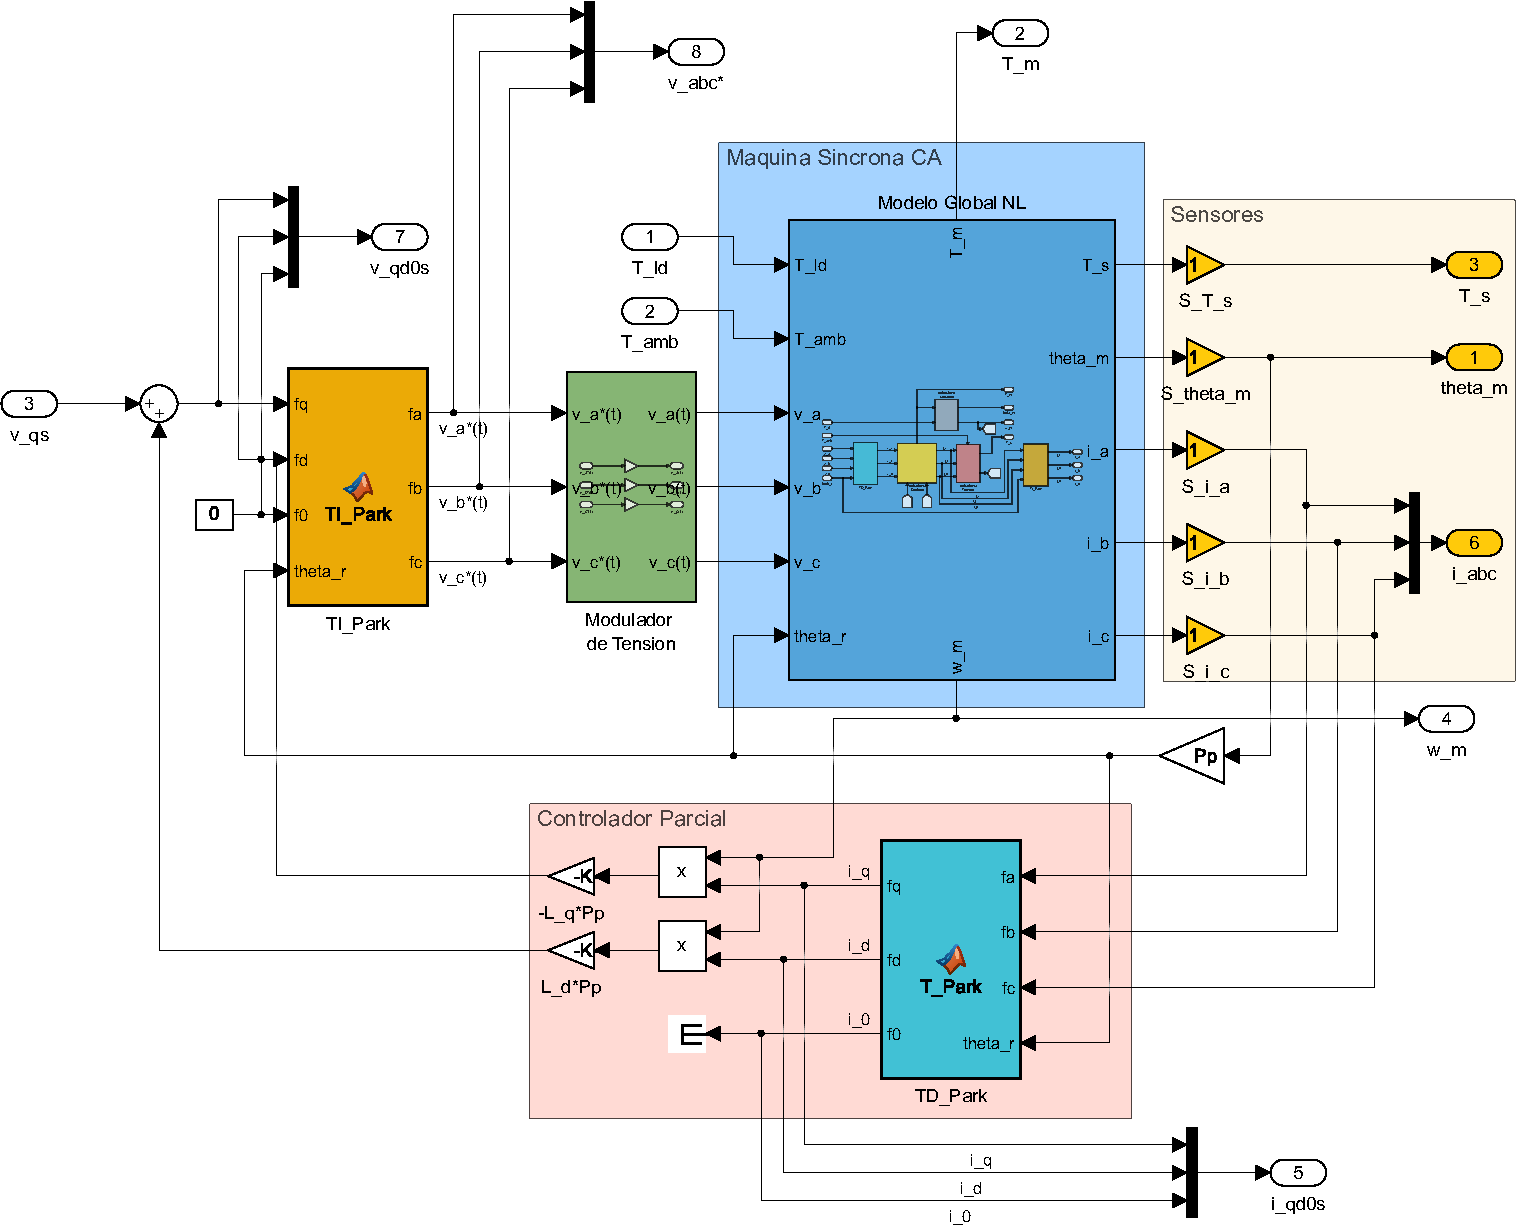
\includegraphics[width=0.95\linewidth]{img/ley_complementaria_q.pdf}
	\caption{Diagrama de bloques del modelo global no lineal del accionamiento con desacoplamiento por realimentación no lineal parcial de estados, implementando la ley de control mínima en el eje $d$ y la ley de control complementaria mínima en el eje $q$ (Modelo global NL con ley de control NL).}
	\label{fig:ley_complementaria_q}
\end{figure}

A partir del modelo LTI equivalente obtenido anteriormente en los incisos I) y II), 
se incorpora ahora la dinámica residual de la corriente de magnetización $i_{ds}^{r}(t)$ y la dinámica térmica del estator $T_s^{\circ}(t)$. 
De esta manera, se construye un modelo LTI equivalente aumentado, cuyo núcleo dinámico sigue siendo el subsistema electromecánico de tercer orden formado por $\theta_m(t)$, $\omega_m(t)$ e $i_{qs}^{r}(t)$. 
El nuevo vector de estado extendido se define entonces de la siguiente manera:

\begin{equation*}
    x_a(t)=
    \begin{bmatrix}
        \theta_m(t)\\
        \omega_m(t)\\
        i_{qs}^{r}(t)\\
        i_{ds}^{r}(t)\\
        T_s^{\circ}(t)
    \end{bmatrix}.
\end{equation*}


Así, la representación en el espacio de estados del modelo global aumentado está regida por el siguiente sistema de ecuaciones diferenciales:

\begin{equation}
	\left\{
	\begin{aligned}
		\dot{\theta}_m(t) &= \omega_m(t)
		\\[2mm]
		\dot{\omega}_m(t) &=
		\frac{1}{J_{eq}}
		\left(
		\frac{3}{2}P_p\lambda_m^{\prime r}i_{qs}^{r}(t)
		-
		b_{eq}\omega_m(t)
		-
		T_{deq}(t)
		\right)
		\\[2mm]
		\frac{di_{qs}^{r}(t)}{dt} &=
		\frac{1}{L_q}
		\left[
		v_{qs}^{r}(t)
		-
		R_{s,\mathrm{REF}}i_{qs}^{r}(t)
		-
		P_p\lambda_m^{\prime r}\omega_m(t)
		\right]
		\\[2mm]
		\frac{di_{ds}^{r}(t)}{dt} &=
		-\frac{R_{s,\mathrm{REF}}}{L_d}i_{ds}^{r}(t)
		\\[2mm]
		\frac{dT_s^{\circ}(t)}{dt} &=
		\frac{1}{C_{ts}}
		\left[
		P_J(t)
		-
		\frac{1}{R_{ts-amb}}
		\left(
		T_s^{\circ}(t)-T_{amb}^{\circ}(t)
		\right)
		\right]
	\end{aligned}
	\right.
	\label{eq:modelo_lti_aumentado}
\end{equation}

En donde la potencia eléctrica disipada por efecto Joule en los devanados del estator se evalua mediante:

\begin{equation}
	P_J(t)=
	\frac{3}{2}R_{s,\mathrm{REF}}
	\left[
	\left(i_{qs}^{r}(t)\right)^2+
	\left(i_{ds}^{r}(t)\right)^2
	\right].
	\label{eq:perdidas_joule_lti_aumentado}
\end{equation}

Es importante destacar que en este modelo se utiliza un valor constante $R_{s,\mathrm{REF}}$, despreciando asi el acoplamiento no lineal entre la temperatura del estator y la resistencia eléctrica de los bobinados. 
En consecuencia, la temperatura $T_s^{\circ}(t)$ actúa como un estado adicional que representa la dinámica térmica del sistema, 
pero no realimenta a las ecuaciones eléctricas mediante una resistencia variable $R_s(T_s^{\circ})$.

La corriente $i_{ds}^{r}(t)$ también se incorpora como un estado adicional debido a que, si bien la ley de control mínima en el eje $d$ impone su decaimiento, 
esta no desaparece instantáneamente. Su dinámica residual queda caracterizada por un sistema de primer orden estable:

\begin{equation*}
\frac{di_{ds}^{r}(t)}{dt}
=
-\frac{R_{s,\mathrm{REF}}}{L_d}i_{ds}^{r}(t),
\end{equation*}

cuyo polo está dado por:

\begin{equation*}
p_d=-\frac{R_{s,\mathrm{REF}}}{L_d}.
\end{equation*}

Dado que los parámetros físicos cumplen que $R_{s,\mathrm{REF}}>0$ y $L_d>0$, se garantiza que $p_d<0$. 
Por lo tanto, $i_{ds}^{r}(t)$ decaerá exponencialmente hacia cero tras cualquier transitorio.

Finalmente, la implementación global de este modelo LTI equivalente aumentado en Simulink se ilustra en la Figura~\ref{fig:modelo_lti_aumentado}.

\begin{figure}[H]
	\centering
	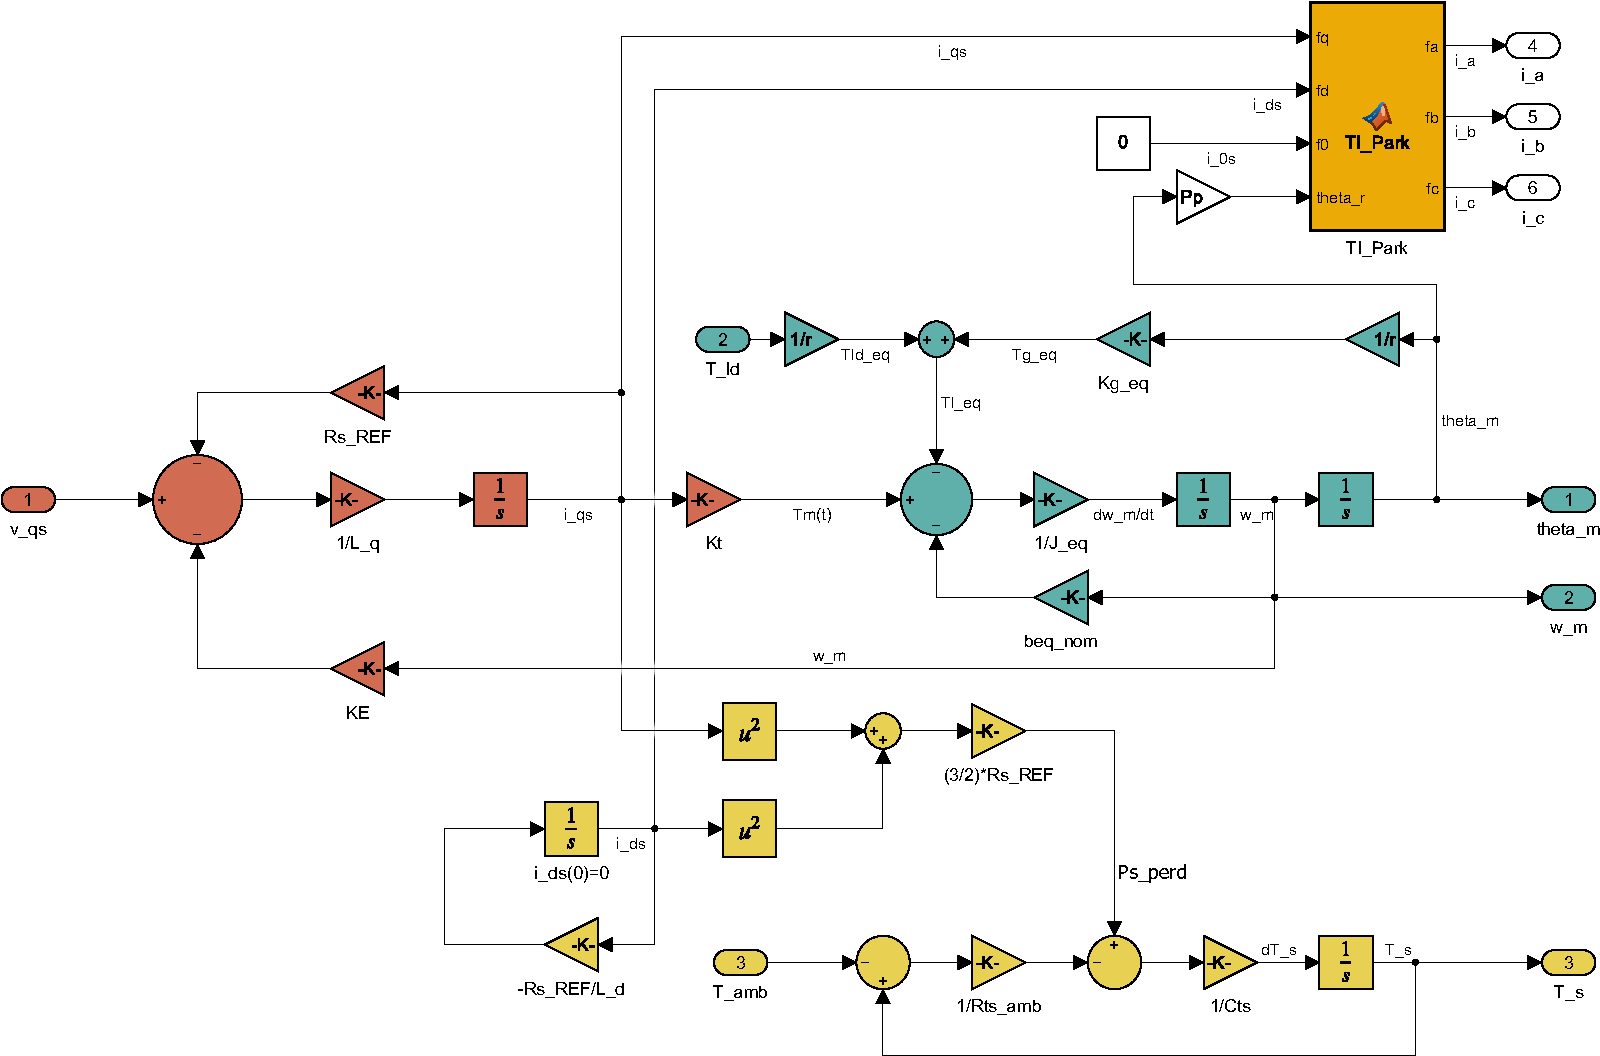
\includegraphics[width=0.95\linewidth]{img/modelo_lti_aumentado.pdf}
	\caption{Diagrama de bloques del modelo LTI equivalente aumentado.}
	\label{fig:modelo_lti_aumentado}
\end{figure}

% ---------------------------------------------------------
\subsubsection{Comparación entre el modelo LTI equivalente aumentado y el modelo LPV}

El modelo LPV y el modelo LTI equivalente aumentado desempeñan roles analíticos fundamentales, aunque distintos, en el estudio del accionamiento. 

Mientras que el modelo LPV, obtenido por linealización Jacobiana del sistema global no lineal conserva la dependencia paramétrica de las matrices de estado respecto al punto de operación, 
el modelo LTI equivalente aumentado se consolida tras aplicar leyes de desacoplamiento y fijar un punto de operación nominal (típicamente bajo la premisa de campo orientado, $I_d^o=0$).

Aunque la variable de operación que se modifica o perturba es la corriente estática del eje directo ($I_{ds}^{ro}$), 
el impacto macroscópico de esta variación (la migración de propiedades) se manifiesta de forma primordial sobre la dinámica del eje de cuadratura ($q$) y la ecuación de movimiento mecánico. 
Esto ocurre debido al fuerte acoplamiento cruzado inherente de la máquina sincrónica. 
Por lo tanto, para establecer una comparativa rigurosa entre ambas representaciones, 
resulta conveniente analizar las ecuaciones electromagnéticas en las que la corriente del eje directo interviene de manera explícita alterando la dinámica de producción de fuerza. 

Recordando, la expresión del torque electromagnético generado por la PMSM está dada por la Ecuacion \eqref{eq:torque_electromagnetico_PMSM}:

\begin{equation*}
	T_m(t)=
	\frac{3}{2}P_p
	\left[
	\lambda_m^{\prime r}+\left(L_d-L_q\right)i_{ds}^{r}(t)
	\right]
	i_{qs}^{r}(t).
\end{equation*}

Al evaluar esta expresión en un entorno de operación donde la corriente de magnetización se asume constante ($i_{ds}^{r}(t)=I_{ds}^{ro}$), 
es posible definir una constante de torque equivalente dependiente del punto de operación:

\begin{equation}
    \boxed{
        K_T(I_{ds}^{ro})=
        \frac{3}{2}P_p
        \left[
        \lambda_m^{\prime r}+\left(L_d-L_q\right)I_{ds}^{ro}
        \right]
    }
    \label{eq:kt_variable_p2}
\end{equation}

lo cual permite reescribir la producción de torque de forma análoga a la de un motor de corriente continua:

\begin{equation}
    T_m(t)=K_T(I_{ds}^{ro})i_{qs}^{r}(t).
	\label{eq:torque_equivalente_f_K_T}
\end{equation}

Por otro lado, la dinámica eléctrica de la tensión del eje de cuadratura ($q$) responde a la Ecuación \eqref{eq:dinamica_tensiones_qd0}:

\begin{equation*}
	v_{qs}^{r}(t)=
	R_s i_{qs}^{r}(t)
	+
	L_q\frac{di_{qs}^{r}(t)}{dt}
	+
	P_p
	\left[
	\lambda_m^{\prime r}+L_d i_{ds}^{r}(t)
	\right]\omega_m(t).
	\label{eq:vq_ke_id}
\end{equation*}

Evaluando nuevamente bajo la condición de régimen permanente en el eje directo ($i_{ds}^{r}(t)=I_{ds}^{ro}$), 
se define la constante de fuerza contraelectromotriz equivalente:

\begin{equation}
    \boxed{
        K_E(I_{ds}^{ro})=
        P_p
        \left(
        \lambda_m^{\prime r}+L_d I_{ds}^{ro}
        \right)
    }
    \label{eq:ke_variable_p2}
\end{equation}

reduciendo la ecuación de la tensión del eje de cuadratura  ($q$) a:

\begin{equation}
    v_{qs}^{r}(t)=
    R_s i_{qs}^{r}(t)
    +
    L_q\frac{di_{qs}^{r}(t)}{dt}
    +
    K_E(I_{ds}^{ro})\omega_m(t).
	\label{eq:tension_q_equivalente_f_K_E}
\end{equation}

De esta formulación se desprende que $K_T(I_{ds}^{ro})$ rige la capacidad de producción de torque del accionamiento, 
mientras que $K_E(I_{ds}^{ro})$ determina la magnitud de la fuerza contraelectromotriz que se opone a la tensión de alimentación en función de la velocidad de giro.

A continuación, se evalúa la migración de propiedades variando $I_{ds}^{ro}$.

% ----------------------------------------------------------------
\paragraph{Caso 1: Operación con campo orientado ideal ($I_{ds}^{ro}=0$).}

Bajo la estrategia de control vectorial clásico de campo orientado, se impone la restricción de anular la corriente de magnetización:

\begin{equation*}
    I_{ds}^{ro}=0.
\end{equation*}

En consecuencia, las constantes dinámicas equivalentes \eqref{eq:kt_variable_p2} y \eqref{eq:ke_variable_p2} colapsan a sus valores nominales estáticos:

\begin{equation*}
	K_T(0)=
	\frac{3}{2}P_p\lambda_m^{\prime r}=K_t,
	\qquad
	K_E(0)=P_p\lambda_m^{\prime r}.
\end{equation*}

Sustituyendo estos valores invariantes, las ecuaciones de torque \eqref{eq:torque_equivalente_f_K_T} y de tensión en el eje de cuadratura \eqref{eq:tension_q_equivalente_f_K_E} 
se simplifican drásticamente:

\begin{equation*}
	T_m(t)=K_t i_{qs}^{r}(t),
\end{equation*}

\begin{equation*}
	v_{qs}^{r}(t)=
	R_s i_{qs}^{r}(t)
	+
	L_q\frac{di_{qs}^{r}(t)}{dt}
	+
	P_p\lambda_m^{\prime r}\omega_m(t).
\end{equation*}

Y la ecuacion mecmecánica equivalente en \eqref{eq:modelo_lti_aumentado} adopta la forma completamente lineal:

\begin{equation*}
	J_{eq}\dot{\omega}_m(t)=
	K_t i_{qs}^{r}(t)
	-
	b_{eq}\omega_m(t)
	-
	T_{deq}(t).
\end{equation*}

Este escenario representa de manera exacta el modelo LTI equivalente aumentado utilizado como modelo nominal de diseño.

\paragraph{Caso 2: Debilitamiento de campo ($I_{ds}^{ro}<0$).}

Cuando se requiere operar el accionamiento por encima de la velocidad base del motor, se impone una corriente de eje directo negativa para debilitar el campo magnético.

\begin{equation*}
    I_{ds}^{ro}<0.
\end{equation*}

Al observar la Ecuacion~\eqref{eq:ke_variable_p2}, como la inductancia $L_d > 0$ y $I_{ds}^{ro}$ es negativo,
el término de acoplamiento se vuelve sustractivo. Esto provoca una disminución de la constante de fuerza contraelectromotriz respecto a su valor nominal:

\begin{equation*}
    K_E(I_{ds}^{ro})<K_E(0).
\end{equation*}

De manera análoga en la Ecuacion~\eqref{eq:kt_variable_p2}, 
dado que en la máquina considerada se cumple la relación de inductancias $L_d > L_q$ (es decir, $L_d - L_q > 0$),
la inyección de corriente negativa genera un término de reluctancia que se opone al torque principal, 
penalizando la constante de producción de torque:

\begin{equation*}
    K_T(I_{ds}^{ro})<K_T(0).
\end{equation*}

Resultando en la siguiente relación de torque-corriente:

\begin{equation*}
    T_m(t)=K_T(I_{ds}^{ro})i_{qs}^{r}(t),
    \qquad \text{para} \quad
    K_T(I_{ds}^{ro})<K_t.
\end{equation*}

Físicamente el debilitamiento de campo reduce la tensión inducida en el estator, 
permitiendo alcanzar velocidades mecánicas superiores sin saturar el límite de tensión del inversor. 
Sin embargo, el costo es una reducción en el torque disponible por cada amperio inyectado en el eje de cuadratura.

\paragraph{Caso 3: Reforzamiento de campo ($I_d^o>0$).}

Si, por el contrario, se inyecta una corriente de eje directo positiva:

\begin{equation*}
    I_{ds}^{ro}>0.
\end{equation*}

Bajo la misma lógica analítica de las Ecuaciones \eqref{eq:ke_variable_p2} y \eqref{eq:kt_variable_p2}, 
los términos algebráicos se vuelven puramente aditivos. Esto amplifica simultáneamente ambas constantes equivalentes:

\begin{equation*}
    K_E(I_{ds}^{ro})>K_E(0),
    \qquad
    K_T(I_{ds}^{ro})>K_T(0).
\end{equation*}

De modo que:

\begin{equation*}
    T_m(t)=K_T(I_{ds}^{ro})i_{qs}^{r}(t),
    \qquad \text{para} \quad
    K_T(I_{ds}^{ro})>K_t.
\end{equation*}

El reforzamiento de campo incrementa la capacidad de producción de torque por amperio.
Sin embargo, esto ocurre a expensas de aumentar la fuerza contraelectromotriz, 
lo que conlleva a que el inversor deba suministrar una tensión mayor para mantener el giro,
limitando la velocidad máxima alcanzable.

Finalmente, es importante destacar que tanto en el debilitamiento como en el reforzamiento de campo, 
se exije apartarse del campo orientado ($I_{ds}^{ro} \neq 0$), lo que incrementará las pérdidas por efecto Joule frente al caso nominal,
puesto que la potencia térmica disipada es proporcional a la suma de los cuadrados de las corrientes de ambos ejes:

\begin{equation}
	P_J(t)=
	\frac{3}{2}R_s
	\left[
	\left(i_{qs}^{r}(t)\right)^2+
	\left(i_{ds}^{r}(t)\right)^2
	\right].
\end{equation}

\paragraph{Migración de propiedades dinámicas.}
En el marco del modelo LPV, modificar el punto de operación $I_{ds}^{ro}$ impacta directamente en múltiples coeficientes de la matriz de estado dinámica $A$.
A modo de ejemplo, el coeficiente:

\begin{equation}
    A_{23}=\frac{K_t+K_{rel}I_{ds}^{ro}}{J_{eq}},
    \label{eq:A23_lpv}
\end{equation}

que caracteriza la influencia de la corriente de cuadratura $i_{qs}^{r}(t)$ sobre la aceleración mecánica, y el coeficiente:

\begin{equation}
    A_{32}=-\frac{P_p\left(\lambda_m^{\prime r}+L_d I_{ds}^{ro}\right)}{L_q},
    \label{eq:A32_lpv}
\end{equation}

que modela el acoplamiento de la velocidad mecánica sobre la dinámica eléctrica del eje $q$,
se ven alterados sustancialmente. Como consecuencia de la variación de estos términos, 
se produce una migración de los polos del sistema, modificando las ganancias, el factor de amortiguamiento y la respuesta transitoria local. 
Por esta razón, el modelo LPV resulta más adecuado para evaluar el rango de validez del modelo LTI y para estudiar la operación en regímenes alejados del punto nominal.

% ---------------------------------------------------------

\subsubsection{Funciones de transferencia del modelo LTI equivalente aumentado}

Las funciones de transferencia se obtienen a partir del subsistema electromecánico extraido del modelo LTI equivalente aumentado, 
definido previamente en el sistema de ecuaciones~\eqref{eq:modelo_lti_aumentado}.
Para ello, es necesario asumir condiciones iniciales nulas en todos los estados.
Físicamente, esto implica que el sistema parte del reposo, sin corrientes almacenadas, 
y en equilibrio térmico con el ambiente ($T_s^\circ(0) = T_{amb}^\circ$):

\begin{equation*}
    \mathbf{x}_a(0) = \mathbf{0}.
\end{equation*}

Esta hipótesis es fundamental, dado que la función de transferencia caracteriza exclusivamente la respuesta forzada del sistema (relacion entrada-salida), 
suprimiento la respuesta libre o transitoria asociada a la energía almacenada inicialmente. 

Para simplificar el álgebra en el dominio de Laplace, 
se utilizarán las constantes electromagnéticas nominales de torque y fuerza contraelectromotriz. 
Como se demostró en las Ecuaciones~\eqref{eq:kt_variable_p2} y~\eqref{eq:ke_variable_p2}, 
al evaluar en el punto de operación de campo orientado ($I_{ds}^{ro} = 0$), estas constantes se reducen a:

\begin{equation*}
    K_t = K_T(0) = \frac{3}{2}P_p\lambda_m^{\prime r}, \qquad K_v = K_E(0) = P_p\lambda_m^{\prime r}.
\end{equation*}

Aplicando la transformada de Laplace a las ecuaciones diferenciaes correspondientes al subsistema electromecánico extraído de~\eqref{eq:modelo_lti_aumentado}, se obtiene:

\begin{align*}
    s \Theta_m(s) &= \Omega_m(s) \\
    (J_{eq}s + b_{eq}) \Omega_m(s) &= K_t I_{qs}^r(s) - T_{deq}(s) \\
    (L_q s + R_{s,\mathrm{REF}}) I_{qs}^r(s) &= V_{qs}^r(s) - K_v \Omega_m(s)
\end{align*}

Remplazando la expresión de la dinámica eléctrica en la ecuación mecánica para aislar la variable $I_{qs}^r(s)$, 
se hace matemáticamente evidente el acoplamiento cruzado generado por la fuerza contraelectromotriz:

\begin{equation*}
    (J_{eq}s + b_{eq}) \Omega_m(s) = \frac{K_t}{L_q s + R_{s,\mathrm{REF}}} \Big[ V_{qs}^r(s) - K_v \Omega_m(s) \Big] - T_{deq}(s).
\end{equation*}

Sustituyendo la relación cinemática $\Omega_m(s) = s \Theta_m(s)$, 
se agrupan los términos para relacionar la posición angular con las entradas del sistema:

\begin{equation}
    s \Big[ (L_q s + R_{s,\mathrm{REF}})(J_{eq}s + b_{eq}) + K_t K_v \Big] \Theta_m(s) = K_t V_{qs}^r(s) - (L_q s + R_{s,\mathrm{REF}}) T_{deq}(s).
\end{equation}

\paragraph{Función de transferencia desde la tensión $v_{qs}^r(t)$ hacia la posición $\theta_m(t)$.}

Considerando que la perturbación es nula ($T_{deq}(t) = 0$), se obtiene la relación directa de la planta principal:

\begin{equation}
    \boxed{
        G_v(s) = \frac{\Theta_m(s)}{V_{qs}^r(s)} = \frac{K_t}{s \Big[ (L_q s + R_{s,\mathrm{REF}})(J_{eq}s + b_{eq}) + K_t K_v \Big]}
    }
    \label{eq:ft_theta_vqs}
\end{equation}

\paragraph{Función de transferencia desde el torque de carga $T_l(t)$ hacia la posición $\theta_m(t)$.}

Asumiendo ahora que la entrada de tensión de control es nula ($V_{qs}^r(s) = 0$), 
y recordando que el torque de carga equivalente reflejado en el eje del motor está mediado por la relación de transmisión del engranaje planetario ($T_{deq}(s) = \frac{1}{r} T_l(s)$), 
se obtiene la función de transferencia ante perturbaciones:

\begin{equation}
    \boxed{
        G_d(s) = \frac{\Theta_m(s)}{T_l(s)} = \frac{-\frac{1}{r} (L_q s + R_{s,\mathrm{REF}})}{s \Big[ (L_q s + R_{s,\mathrm{REF}})(J_{eq}s + b_{eq}) + K_t K_v \Big]}
    }
    \label{eq:ft_theta_tl}
\end{equation}

\paragraph{Polinomio característico del sistema.}
Se observa que ambas funciones de transferencia comparten un mismo denominador complejo. 
A este denominador se lo denomina \textit{polinomio característico} del sistema, 
convencionalmente denotado mediante la letra $\Delta(s)$:

\begin{equation}
    \Delta(s) = s \Big[ (L_q s + R_{s,\mathrm{REF}})(J_{eq}s + b_{eq}) + K_t K_v \Big].
    \label{eq:polinomio_caracteristico_motor}
\end{equation}

Las raíces de $\Delta(s) = 0$ definen unívocamente los polos del sistema electromecánico y, por ende, su estabilidad y dinámica transitoria. 
El término $K_t K_v$ evidencia el fenómeno de amortiguamiento magnético natural, 
producto del acoplamiento cruzado de la fuerza contraelectromotriz.

\paragraph{Estados internos nulos u ocultos en las funciones de transferencia.}
De los cinco estados que componen el modelo LTI equivalente aumentado ($x_a$), existen dos estados específicos que no se ven reflejados ni aportan a las funciones de transferencia obtenidas en~\eqref{eq:ft_theta_vqs} y~\eqref{eq:ft_theta_tl}: la corriente de magnetización $i_{ds}^r(t)$ y la temperatura del estator $T_s^\circ(t)$.

Esta inobservabilidad desde el canal mecánico se explica mediante las siguientes razones analíticas:
\begin{itemize}
    \item \textbf{Inobservabilidad y Desacoplamiento de $i_{ds}^r(t)$:} Como consecuencia directa de la aplicación de la ley de control no lineal en el eje $d$, la dinámica de esta corriente se colapsó a un modo residual de primer orden ($\dot{i}_{ds}^r = -\frac{R_{s,\mathrm{REF}}}{L_d} i_{ds}^r$). Al linealizar el modelo en torno a $I_{ds}^{ro} = 0$, el término cruzado de torque por reluctancia se vuelve nulo. Así, este modo resulta ser autónomo, localmente estable y matemáticamente desacoplado: no es excitado por las entradas de interés ($v_{qs}^r(t)$ o $T_l(t)$) ni altera la trayectoria de la salida mecánica $\theta_m(t)$.
    \item \textbf{Naturaleza No Lineal e Inobservabilidad de $T_s^\circ(t)$:} La dinámica térmica se excita mediante las pérdidas de potencia por efecto Joule $P_J(t)$, las cuales dependen de forma cuadrática (no lineal) de las corrientes de fase. Al aplicar la transformada de Laplace para derivar relaciones estrictamente LTI, esta dependencia no lineal no puede ser representada analíticamente. Adicionalmente, dado que el modelo equivalente asume una resistencia nominal constante $R_{s,\mathrm{REF}}$, las variaciones de temperatura no realimentan el subsistema eléctrico, volviendo al estado térmico un modo estructuralmente inobservable desde la salida $\theta_m(t)$.
\end{itemize}

\paragraph{Síntesis de la Sección 3 (Punto 2).}
A lo largo de este desarrollo se han deducido tres representaciones matemáticas complementarias para el accionamiento mecatrónico, 
cada una con un propósito analítico y de diseño específico.

El \textbf{modelo global no lineal (NL)} representa fielmente la planta física completa en coordenadas virtuales $qd0$, 
permitiendo simular el comportamiento transitorio fuertemente acoplado de la máquina, 
los efectos no lineales de la carga y el calentamiento del estator. 
Es fundamental destacar que es precisamente a este modelo físico original al que se le aplica la linealización por realimentación no lineal. 
Además, al conservar la dinámica completa, es el único entorno en el cual resulta físicamente posible aplicar estrategias de debilitamiento o reforzamiento de campo, 
ya que estas exigen la manipulación directa de la corriente $i_{ds}^{r}(t)$.

Por su parte, el \textbf{modelo lineal con parámetros variables (LPV)}, obtenido mediante linealización Jacobiana, 
preserva la dependencia paramétrica con el punto de operación. 
Su función principal es actuar como la herramienta analítica idónea para estudiar pequeñas variaciones locales y evaluar formalmente cómo migran las propiedades dinámicas del sistema ante las variaciones de magnetización ($I_{ds}^{ro}$).

Finalmente, el \textbf{modelo LTI equivalente aumentado} constituye la planta nominal sobre la cual se diseñarán los futuros controladores. 
Es vital comprender que este modelo no incluye lazos de realimentación en su formulación matemática; 
se trata del modelo lineal equivalente a lazo abierto resultante de asumir que el desacoplamiento de los ejes ya se efectuó exitosamente sobre la planta, 
al cual simplemente se le ha añadido la dinámica residual de la corriente en el eje directo. 
Dado que se construye bajo la premisa estricta de campo orientado ($I_{ds}^{ro} = 0$), 
proporciona un sistema puramente lineal, invariante e independiente del estado de magnetización inicial. 
Como contrapartida lógica, este modelo equivalente no permite estudiar operaciones de debilitamiento o refuerzo de campo, 
puesto que en su estructura la corriente $i_d$ se fuerza permanentemente a cero.


\subsection{Análisis de estabilidad a lazo abierto del modelo LTI equivalente aumentado}

\subsubsection{Determinación de autovalores, polos y ceros}

Para determinar los polos fundamentales del sistema, 
se parte del polinomio característico deducido a partir de las funciones de transferencia en la Ecuación~\eqref{eq:polinomio_caracteristico_motor}:

\begin{equation*}
    \Delta(s) = s \Big[ (L_q s + R_{s,\mathrm{REF}})(J_{eq}s + b_{eq}) + K_t K_v \Big] = 0.
\end{equation*}

Distribuyendo los términos y normalizando respecto al coeficiente de mayor grado ($J_{eq}L_q$), 
el polinomio se expresa como el producto de una raíz nula y una ecuación cuadrática:

\begin{equation}
    s \left[ s^2 + \left( \frac{b_{eq}}{J_{eq}} + \frac{R_{s,\mathrm{REF}}}{L_q} \right) s + \frac{R_{s,\mathrm{REF}} b_{eq} + K_t K_v}{J_{eq} L_q} \right] = 0.
    \label{eq:polinomio_desarrollado_p3}
\end{equation}

De esta expresión se extrae directamente un primer polo en el origen ($p_1 = 0$), 
asociado a la relación cinemática integral entre velocidad y posición. 
En segundo lugar, el término cuadrático entre corchetes define un par de \textbf{polos electromecánicos conjugados}. 
Comparando este término con la forma canónica estándar de un sistema de segundo orden:

\begin{equation*}
    s^2 + 2\zeta_{em}\omega_{n,em}s + \omega_{n,em}^2 = 0,
\end{equation*}

e igualando término a término con el polinomio deducido en la Ecuación~\eqref{eq:polinomio_desarrollado_p3}, 
se establecen las siguientes equivalencias algebraicas:

\begin{align*}
    \omega_{n,em}^2 &= \frac{R_{s,\mathrm{REF}} b_{eq} + K_t K_v}{J_{eq} L_q}, \\[2mm]
    2\zeta_{em}\omega_{n,em} &= \frac{b_{eq}}{J_{eq}} + \frac{R_{s,\mathrm{REF}}}{L_q} = \frac{L_q b_{eq} + R_{s,\mathrm{REF}} J_{eq}}{J_{eq} L_q}.
\end{align*}

Despejando este sistema, se obtienen las expresiones analíticas finales para la frecuencia natural no amortiguada ($\omega_{n,em}$) 
y el factor de amortiguamiento ($\zeta_{em}$):

\begin{equation}
    \omega_{n,em} = \sqrt{\frac{R_{s,\mathrm{REF}} b_{eq} + K_t K_v}{J_{eq} L_q}},
    \label{eq:wn_em_p3}
\end{equation}

\begin{equation}
    \zeta_{em} = \frac{L_q b_{eq} + R_{s,\mathrm{REF}} J_{eq}}{2 \sqrt{J_{eq} L_q (R_{s,\mathrm{REF}} b_{eq} + K_t K_v)}}.
    \label{eq:zeta_em_p3}
\end{equation}

Por consiguiente, las raíces del polinomio electromecánico arrojan un polo en el origen ($p_1 = 0$) y un par de polos complejos conjugados:

\begin{equation}
    p_{2,3} = -\zeta_{em}\omega_{n,em} \pm j \omega_{n,em}\sqrt{1-\zeta_{em}^2} = -\sigma_{em} \pm j\omega_{d,em}.
\end{equation}

Para completar el conjunto de autovalores del modelo LTI equivalente aumentado, es indispensable incluir la dinámica de los estados que resultan inobservables desde las funciones de transferencia hacia la posición. Como se justificó en la sección anterior, la corriente del eje $d$ y la temperatura del estator aportan dos polos reales adicionales:

\begin{itemize}
    \item \textbf{Polo eléctrico residual (eje $d$):} $p_4 = p_d = -R_{s,\mathrm{REF}}/L_d$. Su constante de tiempo asociada es $\tau_d = L_d / R_{s,\mathrm{REF}}$.
    \item \textbf{Polo térmico:} $p_5 = p_T = -1/(R_{ts-amb}C_{ts})$. Su constante de tiempo característica es $\tau_T = R_{ts-amb}C_{ts}$.
\end{itemize}

\paragraph{Determinación de ceros.}
A partir de las funciones de transferencia~\eqref{eq:ft_theta_vqs} y~\eqref{eq:ft_theta_tl}, se determinan los ceros del sistema dependiendo de la entrada de excitación:

\begin{itemize}
    \item Para la entrada de tensión de control $V_{qs}^r(s)$, la transferencia de lazo directo $G_v(s)$ posee un numerador constante ($K_t$), por lo que \textbf{no presenta ceros finitos}. Su respuesta transitoria está dictaminada enteramente por la dinámica de los polos.
    \item Para la entrada de perturbación de carga mecánica $T_l(s)$, la transferencia $G_d(s)$ presenta un \textbf{único cero finito} en el semiplano izquierdo asociado a la dinámica inductiva del estator, ubicado en:
    \begin{equation}
        z_d = -\frac{R_{s,\mathrm{REF}}}{L_q}.
    \end{equation}
\end{itemize}

\paragraph{Evaluación numérica y correspondencia física.}
A partir de las expresiones analíticas deducidas, el análisis de estabilidad a lazo abierto se concreta evaluando numéricamente los polos y ceros del modelo LTI equivalente aumentado. Reemplazando los parámetros nominales del accionamiento en las fórmulas previamente obtenidas, se determinan los índices de desempeño dinámico.

En primer lugar, evaluando las Ecuaciones~\eqref{eq:wn_em_p3} y~\eqref{eq:zeta_em_p3}, la frecuencia natural y el factor de amortiguamiento del subsistema electromecánico resultan:
\begin{align*}
    \omega_{n,em} &= 174.10 \, \mathrm{rad/s} \quad (27.71 \, \mathrm{Hz}) \\
    \zeta_{em} &= 0.5082
\end{align*}
Al tratarse de un sistema subamortiguado ($0 < \zeta_{em} < 1$), el par de polos complejos conjugados dominante se ubica en:
\begin{equation}
    p_{2,3} = -88.49 \pm j149.94 \, \mathrm{rad/s}.
\end{equation}

Por otro lado, el único cero finito del sistema, introducido de forma exclusiva por la transferencia de perturbación $G_d(s)$, se localiza en:
\begin{equation}
    z_d = -\frac{R_{s,\mathrm{REF}}}{L_q} = -175.86 \, \mathrm{rad/s}.
\end{equation}

Finalmente, las raíces correspondientes a los modos inobservables desde la variable de posición (la dinámica de magnetización residual y la dinámica térmica) se evalúan como:
\begin{align*}
    p_d &= -\frac{R_{s,\mathrm{REF}}}{L_d} = -154.55 \, \mathrm{rad/s}, \\
    p_T &= -\frac{1}{R_{ts-amb}C_{ts}} = -0.0083 \, \mathrm{rad/s}.
\end{align*}

Todos estos resultados numéricos, en conjunto con el polo integrador cinemático ($p_1=0$), se consolidan en la Tabla~\ref{tab:autovalores_lti_num}, en la cual se detallan sus constantes de tiempo asociadas y su efecto fenoménico sobre la planta.

\begin{table}[H]
    \centering
    \caption{Singularidades numéricas y propiedades del modelo LTI equivalente a lazo abierto.}
    \label{tab:autovalores_lti_num}
    \begin{tabular}{>{\raggedright\arraybackslash}p{3.8cm} >{\centering\arraybackslash}p{4cm} >{\centering\arraybackslash}p{2.5cm} >{\raggedright\arraybackslash}p{4.5cm}}
        \toprule
        \textbf{Subsistema / Modo} & \textbf{Ubicación en $s$ (\si{\radian\per\second})} & \textbf{Cte. de Tiempo} & \textbf{Efecto Dinámico} \\
        \midrule
        Cinemático (Integrador) & $p_1 = 0.00$ & $\infty$ & Posición libre sin resorte de retorno. Origina inestabilidad BIBO. \\
        \addlinespace
        Electromecánico (Dominante) & $p_{2,3} = -88.49 \pm j149.94$ & $\tau_{em} = \SI{11.3}{\milli\second}$ & Dinámica acoplada subamortiguada. Decaimiento de la envolvente oscilatoria. \\
        \addlinespace
        Eléctrico residual Eje $d$ & $p_d = -154.55$ & $\tau_d = \SI{6.5}{\milli\second}$ & Decaimiento autónomo y estable de la corriente de magnetización. \\
        \addlinespace
        Térmico (Estator) & $p_T = -0.0083$ & $\tau_T = \SI{120.0}{\second}$ & Inercia calórica de extrema lentitud. Desacoplada del transitorio. \\
        \midrule
        Cero (Entrada $T_l$) & $z_d = -175.86$ & $\tau_q = \SI{5.7}{\milli\second}$ & Adelanto de fase local ante perturbación de torque de carga. \\
        \bottomrule
    \end{tabular}
\end{table}

\begin{figure}[H]
	\centering
	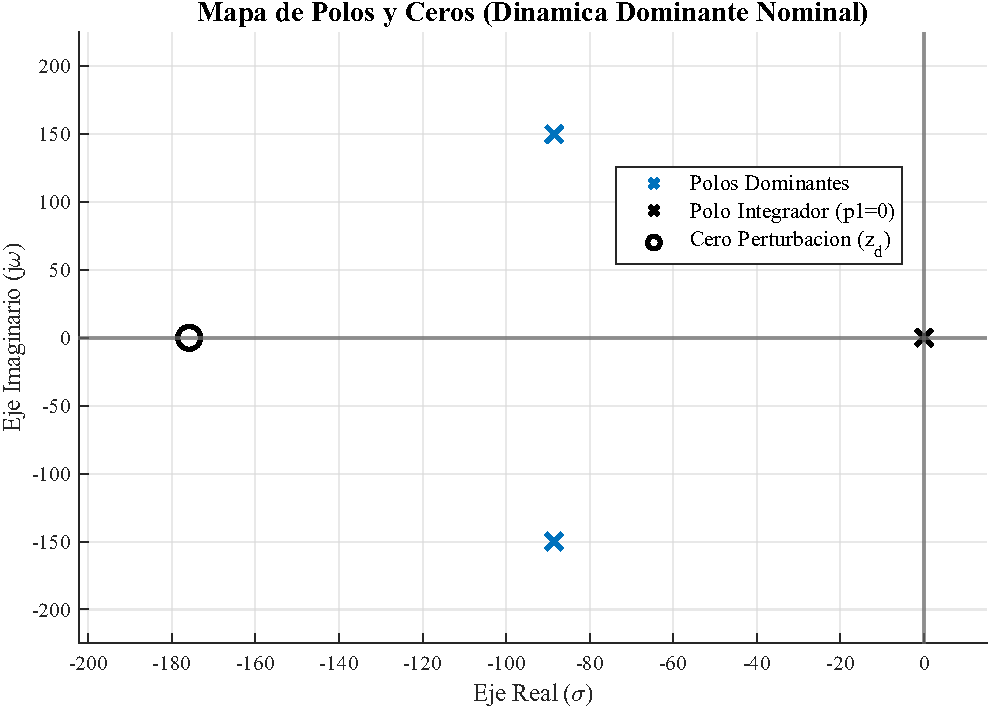
\includegraphics[width=0.95\linewidth]{img/mapa_pz_nominal.pdf}
	\caption{Mapa de polos y ceros nominal del modelo LTI equivalente.}
	\label{fig:pzmap_nominal}
\end{figure}

\paragraph{Conclusión sobre la estabilidad a lazo abierto.}
La evaluación de la estabilidad del sistema requiere un análisis exhaustivo tanto de sus modos observables como de los inobservables. 
El análisis espectral de los autovalores revela que el sistema global es \textbf{marginalmente estable} a lazo abierto. 
Esta condición es impuesta de manera exclusiva por la inercia integradora de la posición ($p_1 = 0$). 
Como consecuencia de este polo, cualquier perturbación de carga $T_l(t)$ o entrada de tensión $v_{qs}^r(t)$ constante y sostenida en el tiempo provocará un desplazamiento angular ilimitado de tipo rampa, 
indicando formalmente que el sistema \textit{no posee estabilidad BIBO (Bounded-Input Bounded-Output)} para la variable de salida $\theta_m(t)$.

Por otro lado, al analizar la estabilidad interna del modelo aumentado, 
se constata que todos los autovalores restantes ($p_{2,3}, p_d, p_T$) se ubican estrictamente en el semiplano izquierdo del plano complejo $s$. 
Esto incluye tanto a los polos electromecánicos visibles desde la transferencia principal, 
como a los modos residuales desacoplados ($i_{ds}^r$ y $T_s^\circ$) que, 
si bien no aparecen de forma directa en las funciones de transferencia hacia la posición, 
garantizan el decaimiento estable de las corrientes y la temperatura hacia sus valores de equilibrio. 
Por consiguiente, se concluye que la derivada de la posición (la velocidad angular $\omega_m$) y todos los estados internos de la máquina sí gozan de \textbf{estabilidad asintótica parcial}.

Este comportamiento dual, donde la velocidad y los estados internos se estabilizan naturalmente mientras la posición diverge de forma libre, 
es una característica inherente a los servoaccionamientos electromecánicos. 
Este análisis justifica matemáticamente la necesidad imperativa de diseñar y cerrar un lazo de control de posición externo en las etapas posteriores del proyecto.

% ---------------------------------------------------------
\subsubsection{3.b) Estabilidad y migración de propiedades (Incertidumbre paramétrica)}

Las aplicaciones mecatrónicas reales están sometidas a incertidumbres operativas. 
La consigna indica evaluar la migración de propiedades de la planta ante variaciones de carga. 
Para lograr una caracterización robusta, 
este análisis se dividirá aislando las fuentes de incertidumbre, 
evaluando secuencialmente el impacto de la inercia de la carga útil ($m_l$), 
la fricción viscosa ($b_l$) y las variaciones térmicas en la resistencia estatórica ($R_s$).

\paragraph{3.b.1) Migración ante variaciones de inercia de carga ($m_l$).}

Para aislar el efecto de la masa inercial, se asume una fricción de carga nominal ($b_l = 0.10\,\si{\newton\meter\second\per\radian}$) y una temperatura estatórica constante. 
Se procede a realizar un barrido de la masa útil en su rango especificado:

\begin{equation*}
    m_l \in [0,\;1.5]\,\si{\kilogram},
\end{equation*}

Como se definió en el modelado mecánico, un incremento de $m_l$ genera un aumento lineal en la inercia rotacional total equivalente ($J_{eq}$). Es vital destacar una sutileza teórica fundamental de este modelo LTI: si bien la variación de la masa útil $m_l$ también modifica el coeficiente gravitacional de la carga, la gravedad actúa en este sistema puramente como una \textit{perturbación externa} de torque ($T_{deq}$) y no como una realimentación linealizada de posición (resorte equivalente). En consecuencia, las variaciones gravitacionales afectan la amplitud de la respuesta forzada de posición, pero \textbf{no modifican en absoluto la ubicación de los polos del sistema}. 

Por lo tanto, la inercia $J_{eq}$ es el único factor capaz de perturbar las raíces dinámicas. Al proyectar sus variaciones sobre las Ecuaciones~\eqref{eq:wn_em_p3} y~\eqref{eq:zeta_em_p3}, se constata que los polos electromecánicos $p_{2,3}$ son los únicos que experimentan una migración espacial. Los resultados de este barrido se sintetizan en la Tabla~\ref{tab:migracion_ml}.

\begin{table}[H]
    \centering
    \caption{Migración de los polos dominantes $p_{2,3}$ ante variaciones de la masa de carga útil $m_l$, asumiendo $b_l=0.10\,\si{\newton\meter\second\per\radian}$.}
    \label{tab:migracion_ml}
    \begin{tabular}{>{\raggedright\arraybackslash}p{2cm} >{\centering\arraybackslash}p{2.5cm} >{\centering\arraybackslash}p{2cm} >{\centering\arraybackslash}p{1.5cm} >{\centering\arraybackslash}p{4cm}}
        \toprule
        \textbf{$m_l$ [kg]} & \textbf{$J_{eq}$ [\si{\kilogram\meter\squared}]} & \textbf{$\omega_{n,em}$ [rad/s]} & \textbf{$\zeta_{em}$} & \textbf{Polos $p_{2,3}$ [rad/s]} \\
        \midrule
        $0.00$ & $1.978\times10^{-5}$ & $174.10$ & $0.508$ & $-88.49 \pm j149.94$ \\
        \addlinespace
        $0.75$ & $3.281\times10^{-5}$ & $135.20$ & $0.627$ & $-84.77 \pm j105.31$ \\
        \addlinespace
        $1.50$ & $4.583\times10^{-5}$ & $114.43$ & $0.725$ & $-83.08 \pm j78.81$ \\
        \bottomrule
    \end{tabular}
\end{table}

\begin{figure}[H]
	\centering
	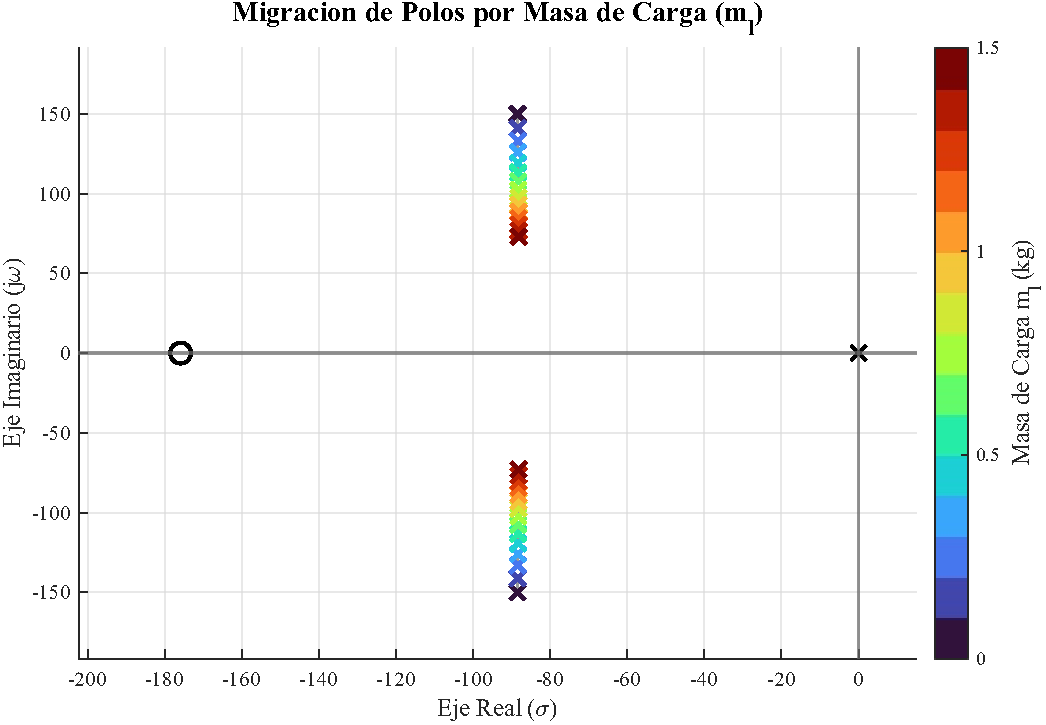
\includegraphics[width=0.95\linewidth]{img/mapa_pz_migracion_ml.pdf}
	\caption{Migración de los polos electromecánicos $p_{2,3}$ en el plano $s$ ante el aumento progresivo de la masa de carga útil $m_l$.}
	\label{fig:mapa_pz_migracion_ml}
\end{figure}


A partir del mapa de polos de la Figura~\ref{fig:mapa_pz_migracion_ml} y del análisis paramétrico, se concluye que:

\begin{enumerate}
    \item \textbf{Ralentización de la respuesta dinámica:} 
	A medida que la inercia $J_{eq}$ se incrementa por efecto de la masa, 
	la frecuencia natural $\omega_{n,em}$ disminuye. 
	Físicamente, una inercia mayor requiere una cantidad superior de torque para alcanzar la misma aceleración, 
	volviendo al accionamiento inherentemente más lento ante excitaciones.

    \item \textbf{Aumento del amortiguamiento relativo:} 
	La trayectoria descendente (hacia el eje real) de los polos indica que el sistema se vuelve \textit{menos oscilatorio} frente a cargas pesadas. 
	Matemáticamente, según la Ecuación~\eqref{eq:zeta_em_p3}, dado que $R_{s,\mathrm{REF}}$ domina el numerador del amortiguamiento, 
	el factor $\zeta_{em}$ resulta ser casi proporcional a $\sqrt{J_{eq}}$. 
	Así, al aumentar la inercia, se potencia la disipación relativa de la energía transitoria frente al movimiento armónico.
    
	\item La inercia añadida no altera el tiempo de establecimiento de manera proporcional a la ralentización, 
	dado que la parte real del polo ($\sigma_{em} \approx -88\,\text{rad/s}$) se mantiene contenida en una vecindad estrecha, 
	garantizando que \textbf{la estabilidad asintótica nunca corre peligro} de invadir el semiplano derecho.
\end{enumerate}

\paragraph{3.b.2) Migración ante variaciones de fricción viscosa ($b_l$).}

En segunda instancia, se aísla el efecto de la incertidumbre en la fricción viscosa de la articulación mecánica, manteniendo la masa en su valor nominal en vacío ($m_l = 0\,\si{\kilogram}$). Se evalúa el rango especificado de tolerancia operativa:

\begin{equation*}
    b_l \in [0.07,\;0.13]\,\frac{\si{\newton\meter\second}}{\si{\radian}}.
\end{equation*}

A diferencia del caso anterior, la variación de $b_l$ únicamente altera el coeficiente de fricción viscosa equivalente reflejado en el eje del motor ($b_{eq}$), dejando inalterada la inercia total ($J_{eq}$). Sustituyendo analíticamente este incremento en las Ecuaciones~\eqref{eq:wn_em_p3} y~\eqref{eq:zeta_em_p3}, se tabula el desplazamiento paramétrico de los polos electromecánicos $p_{2,3}$ (ver Tabla~\ref{tab:migracion_bl_incertidumbre}).

\begin{table}[H]
    \centering
    \caption{Migración de los polos dominantes $p_{2,3}$ ante variaciones de la fricción viscosa $b_l$, asumiendo $m_l=0\,\si{\kilogram}$.}
    \label{tab:migracion_bl_incertidumbre}
    \begin{tabular}{>{\raggedright\arraybackslash}p{2.2cm} >{\centering\arraybackslash}p{2.5cm} >{\centering\arraybackslash}p{2cm} >{\centering\arraybackslash}p{1.5cm} >{\centering\arraybackslash}p{4cm}}
        \toprule
        \textbf{$b_l$} \newline [\si{\newton\meter\second\per\radian}] & \textbf{$b_{eq}$} \newline [\si{\newton\meter\second\per\radian}] & \textbf{$\omega_{n,em}$} [rad/s] & \textbf{$\zeta_{em}$} & \textbf{Polos $p_{2,3}$ [rad/s]} \\
        \midrule
        $0.070$ (Mín) & $1.986\times10^{-5}$ & $174.05$ & $0.5081$ & $-88.43 \pm j149.91$ \\
        \addlinespace
        $0.100$ (Nom) & $2.194\times10^{-5}$ & $174.10$ & $0.5082$ & $-88.49 \pm j149.94$ \\
        \addlinespace
        $0.130$ (Máx) & $2.403\times10^{-5}$ & $174.16$ & $0.5084$ & $-88.54 \pm j159.97$ \\
        \bottomrule
    \end{tabular}
\end{table}

\begin{figure}[H]
	\centering
	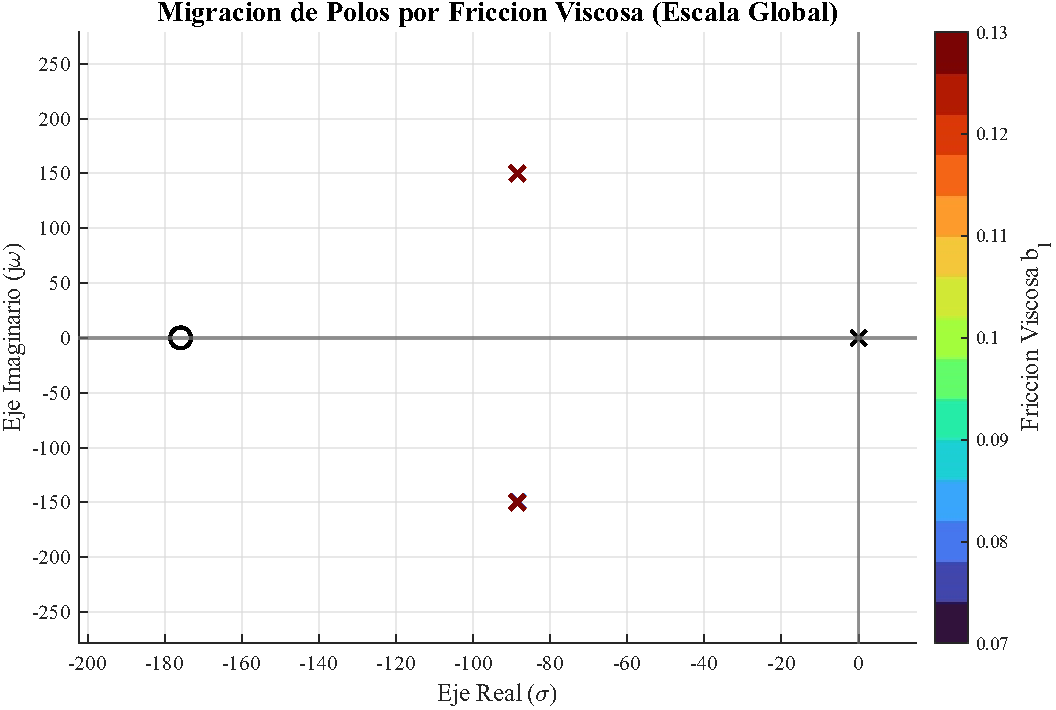
\includegraphics[width=0.95\linewidth]{img/mapa_pz_migracion_bl_global.pdf}
	\caption{Visión general de la migración de los polos electromecánicos $p_{2,3}$ en el plano $s$ ante variaciones de la fricción viscosa de carga $b_l$.}
	\label{fig:mapa_pz_migracion_bl}
\end{figure}

\begin{figure}[H]
	\centering
	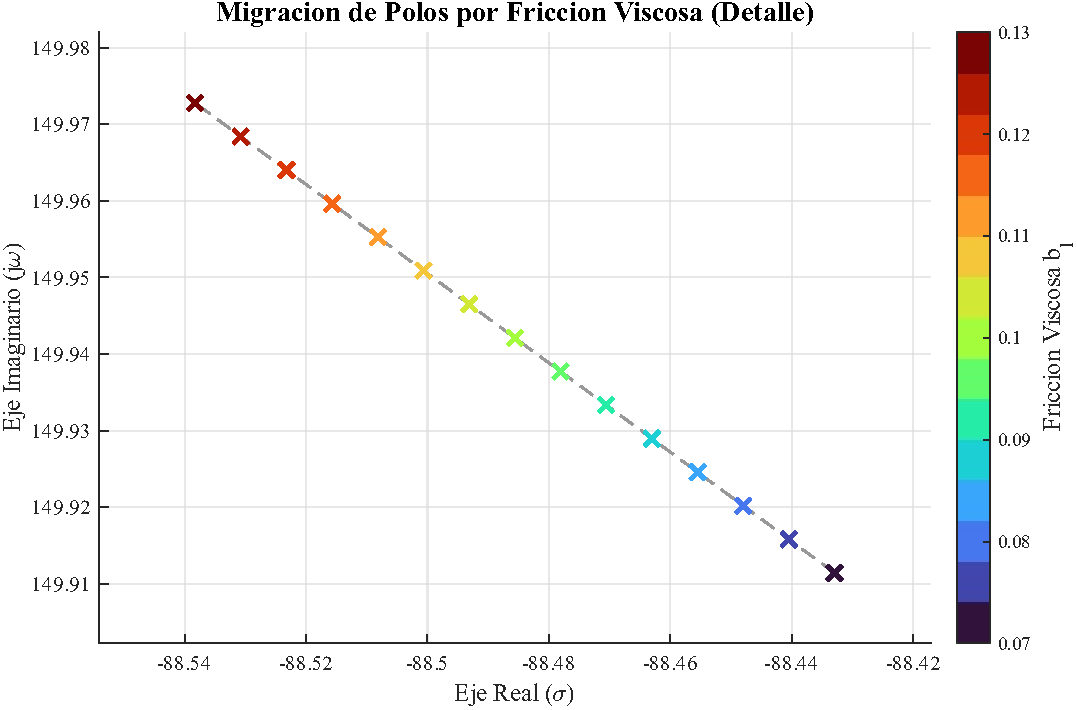
\includegraphics[width=0.95\linewidth]{img/mapa_pz_migracion_bl_zoom.pdf}
	\caption{Detalle de la migración de los polos electromecánicos $p_{2,3}$ en el plano $s$ ante variaciones de la fricción viscosa de carga $b_l$.}
	\label{fig:mapa_pz_migracion_bl_zoom}
\end{figure}


A la luz de los datos obtenidos y las Figuras~\ref{fig:mapa_pz_migracion_bl} y~\ref{fig:mapa_pz_migracion_bl_zoom}, se extraen las siguientes observaciones teóricas:

\begin{enumerate}
    \item \textbf{Alta atenuación cinemática (Aislamiento mecánico):} 
	El impacto de la incertidumbre de fricción sobre la dinámica del motor es virtualmente insignificante. 
	Esta propiedad de insensibilidad no es casual, sino que es consecuencia directa de la altísima relación de reducción de la caja planetaria ($r = 120$). 
	Al reflejarse hacia el estator, cualquier variación de la fricción en la carga queda dividida por un factor $r^2 = 14400$, 
	filtrando eficazmente la incertidumbre externa frente a los parámetros base del accionamiento.
    \item \textbf{Migración predominantemente horizontal:} 
	En la vista ampliada (Figura~\ref{fig:mapa_pz_migracion_bl_zoom}), 
	se aprecia que el leve aumento neto en $b_{eq}$ arrastra a los polos horizontalmente hacia la izquierda y hacia abajo
	incrementando sutilmente la tasa de decaimiento exponencial ($\sigma_{em}$) sin alterar prácticamente el perfil oscilatorio global ($\zeta_{em} \approx 0.508$). 
	Físicamente, un sistema marginalmente más viscoso disipa energía transitoria de manera ligeramente superior, 
	afianzando la estabilidad asintótica sin generar lentitud adicional.
\end{enumerate}

\paragraph{3.b.3) Migración ante variaciones de resistencia estatórica ($R_s$) por temperatura.}

Como última fuente de incertidumbre, se evalúa el impacto del calentamiento térmico del motor sobre la dinámica a lazo abierto. 
Al operar el accionamiento, las pérdidas por efecto Joule elevan la temperatura del estator ($T_s$) desde un valor ambiental/nominal (asumido en $20\,^\circ\mathrm{C}$) hasta la temperatura máxima de diseño ($115\,^\circ\mathrm{C}$). 

Este gradiente térmico provoca un incremento lineal directo sobre la resistencia eléctrica de las bobinas de cobre ($R_s$). A diferencia de los parámetros de carga evaluados anteriormente, la resistencia $R_s$ tiene un impacto profundo tanto en el canal eléctrico como en el electromecánico. Al proyectar su variación desde $1.02\,\si{\ohm}$ hasta $1.32\,\si{\ohm}$ (ver Tabla~\ref{tab:migracion_rs_incertidumbre}), se ven afectados el polo residual $p_d$, el cero de perturbación $z_d$ y el par de polos dominantes $p_{2,3}$.

\begin{table}[H]
    \centering
    \caption{Migración de polos y ceros ante el calentamiento resistivo del estator (Rango de $20^\circ\mathrm{C}$ a $115^\circ\mathrm{C}$), asumiendo carga nominal nula.}
    \label{tab:migracion_rs_incertidumbre}
    \begin{tabular}{>{\raggedright\arraybackslash}p{2.5cm} >{\centering\arraybackslash}p{1.5cm} >{\centering\arraybackslash}p{2cm} >{\centering\arraybackslash}p{1.5cm} >{\centering\arraybackslash}p{3cm} >{\centering\arraybackslash}p{2.5cm}}
        \toprule
        \textbf{Temp. Estator} & \textbf{$R_s$ [\si{\ohm}]} & \textbf{$\omega_{n,em}$} \newline [rad/s] & \textbf{$\zeta_{em}$} & \textbf{Polos $p_{2,3}$} \newline [rad/s] & \textbf{Cero $z_d$ y Polo $p_d$} [rad/s] \\
        \midrule
        $20\,^\circ\mathrm{C}$ (Nom) & $1.02$ & $174.10$ & $0.508$ & $-88.49 \pm j149.94$ & $z_d = -175.86$ \newline $p_d = -154.55$ \\
        \addlinespace
        $67.5\,^\circ\mathrm{C}$ (Media) & $1.21$ & $174.21$ & $0.601$ & $-104.77 \pm j139.18$ & $z_d = -208.44$ \newline $p_d = -183.18$ \\
        \addlinespace
        $115\,^\circ\mathrm{C}$ (Máx) & $1.40$ & $174.31$ & $0.695$ & $-121.06 \pm j125.41$ & $z_d = -241.02$ \newline $p_d = -211.80$ \\
        \bottomrule
    \end{tabular}
\end{table}

\begin{figure}[H]
	\centering
	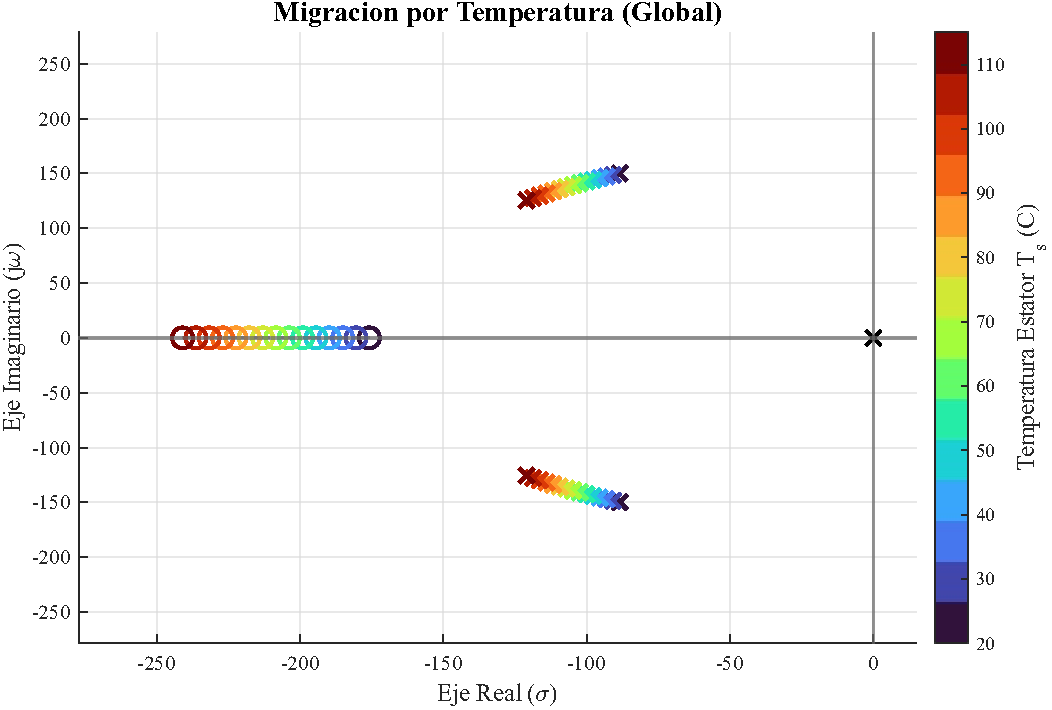
\includegraphics[width=0.95\linewidth]{img/mapa_pz_migracion_Ts_global.pdf}
	\caption{Migración general de polos y ceros en el plano $s$ ante el aumento de la temperatura del estator (y por consiguiente, de $R_s$).}
	\label{fig:mapa_pz_migracion_Rs}
\end{figure}

\begin{figure}[H]
	\centering
	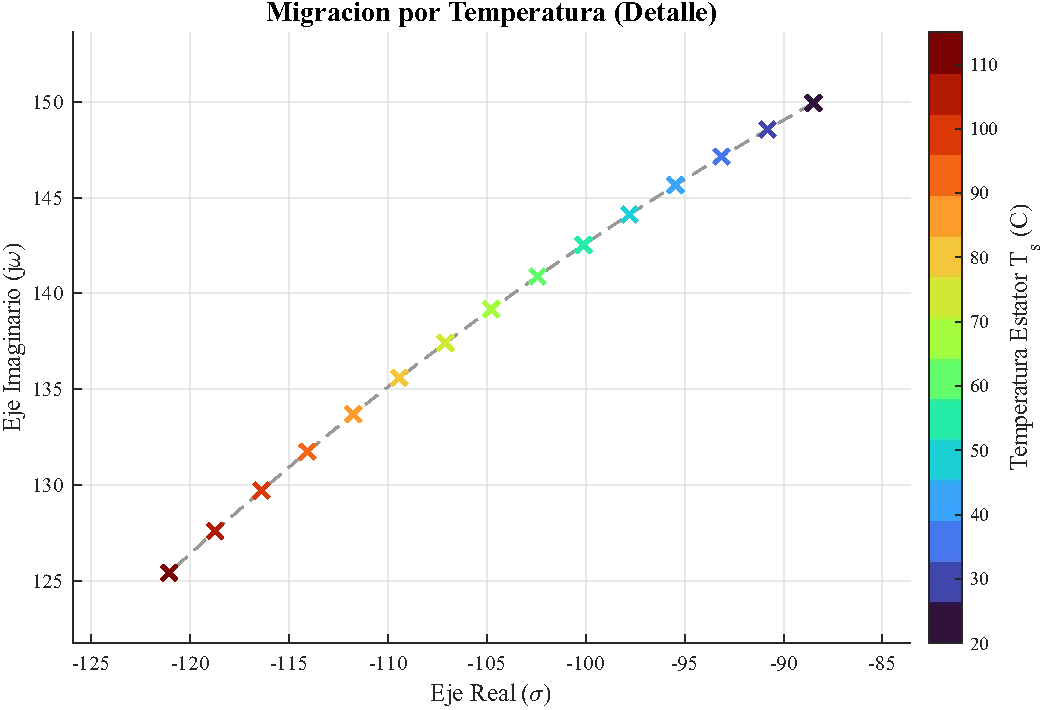
\includegraphics[width=0.95\linewidth]{img/mapa_pz_migracion_Ts_zoom.pdf}
	\caption{Detalle ampliado de la significativa migración del par dominante electromecánico $p_{2,3}$ ante el calentamiento del motor.}
	\label{fig:mapa_pz_migracion_Rs_zoom}
\end{figure}

Analizando los mapas de polos de las Figuras~\ref{fig:mapa_pz_migracion_Rs} y~\ref{fig:mapa_pz_migracion_Rs_zoom}, el calentamiento arroja conclusiones contraintuitivas pero rigurosamente justificadas por el modelo matemático:

\begin{enumerate}
    \item \textbf{Aumento contundente del amortiguamiento:} La observación más destacable radica en el desplazamiento diagonal hacia el origen del par $p_{2,3}$. Al aumentar $R_s$, el factor $\zeta_{em}$ se eleva de forma casi lineal (desde $0.508$ hasta $0.658$), convirtiendo a un motor "caliente" en un sistema significativamente \textit{menos oscilatorio} y \textit{más rápido para estabilizarse} (la envolvente pasa de $-88$ a $-114\,\text{rad/s}$). Físicamente, un devanado con mayor resistencia eléctrica disipa de manera más veloz la energía electromagnética del transitorio por medio del efecto Joule ($I^2R$), operando como un freno eléctrico natural frente al fenómeno oscilatorio.
    \item \textbf{Aceleración de las dinámicas eléctricas:} Como era de esperar, tanto el cero del eje en cuadratura ($z_d$) como el polo residual directo ($p_d$) se alejan profundamente por el eje real negativo. Esto reduce las constantes de tiempo eléctricas ($\tau_q, \tau_d$), volviendo a las corrientes de magnetización más rápidas en extinguirse ante perturbaciones en alta temperatura.
\end{enumerate}

\paragraph{Síntesis del Análisis de Estabilidad a Lazo Abierto.}

El modelo LTI equivalente aumentado presenta cinco autovalores: un polo en el origen ($p_1=0$) asociado al modo cinemático integrador; un par complejo conjugado dominante ($p_{2,3}$) representativo del modo electromecánico subamortiguado; y dos polos reales, uno rápido correspondiente a la dinámica eléctrica residual del eje $d$ ($p_d$) y otro extremadamente lento para la dinámica térmica estatórica ($p_T$).

Al evaluar la condición operativa nominal y los escenarios de máxima perturbación (incertidumbre de carga mecánica y severidad térmica), todos los autovalores internos, excluyendo el integrador, conservan sistemáticamente una parte real estrictamente negativa. Esto permite afirmar que el sistema a lazo abierto presenta \textbf{estabilidad asintótica parcial}, garantizando que la dinámica propia de la máquina no es intrínsecamente inestable. Sin embargo, la presencia fundamental del polo $p_1=0$ condiciona al accionamiento a una \textbf{estabilidad marginal}, resultando inestable en el sentido BIBO para la posición angular $\theta_m(t)$, obligando así al diseño de una compensación por lazo de control.

A partir de la migración paramétrica evaluada en los tres escenarios de incertidumbre (masa, fricción y temperatura), se desprenden las siguientes conclusiones fundamentales sobre la robustez pasiva de la planta:

\begin{enumerate}
    \item \textbf{Ralentización inercial (Variación de $m_l$):} El incremento de la masa útil traslada los polos electromecánicos hacia el origen, disminuyendo drásticamente la frecuencia natural ($\omega_{n,em}$). Físicamente, el sistema obedece a la inercia rotacional: una carga pesada demanda más torque para acelerar, volviendo al accionamiento inherentemente más lento para responder ante excitaciones.
    
    \item \textbf{Aislamiento frente a fricción externa (Variación de $b_l$):} El impacto de la incertidumbre en la fricción de la articulación es insignificante debido a la alta atenuación cinemática del reductor planetario (filtro proporcional a $1/r^2$). Su efecto se limita a un desplazamiento horizontal minúsculo que mejora marginalmente el decaimiento de las oscilaciones sin generar lentitud adicional.
    
    \item \textbf{Aumento contundente del amortiguamiento por temperatura (Variación de $R_s$):} Paradójicamente, el calentamiento del motor actúa como un freno eléctrico. La elevación de la resistencia estatórica potencia la disipación por efecto Joule, incrementando sustancialmente el factor de amortiguamiento ($\zeta_{em}$ de $0.508$ a $0.695$) y convirtiendo al accionamiento en un sistema marcadamente menos oscilatorio.
    
    \item \textbf{Conservación estricta de la estabilidad:} En todos los escenarios de incertidumbre evaluados, la parte real de los polos electromecánicos ($\sigma_{em} < 0$) y residuales se mantiene firmemente anclada en el semiplano izquierdo. Se concluye que la planta pasiva es intrínsecamente robusta y no corre riesgo de inestabilizarse ante el rango de perturbaciones especificado.
\end{enumerate}

Estos hallazgos definen los criterios críticos para la síntesis del control: el futuro controlador a lazo cerrado deberá poseer el ancho de banda suficiente para acelerar el comportamiento aletargado de la planta a plena carga, a la vez que compense las variaciones de ganancia introducidas por las caídas óhmicas en régimen de alta temperatura, garantizando un seguimiento rápido de las trayectorias independientemente de las condiciones operativas del manipulador.

============== HASTA ACA ================
\subsection{Punto 4: Análisis de observabilidad completa de estado del modelo LTI equivalente aumentado}

En este punto se analiza la observabilidad completa de estado del modelo LTI equivalente aumentado obtenido en el punto 2.c.VI, considerando inicialmente como salida medida la posición angular del rotor del motor $\theta_m(t)$. El objetivo es determinar si, a partir de dicha medición, es posible reconstruir todos los estados internos del modelo aumentado.

El vector de estado considerado es

\begin{equation}
	x_{LTI}(t)=
	\begin{bmatrix}
		\theta_m(t)\\
		\omega_m(t)\\
		i_q(t)\\
		i_d(t)\\
		T_s^\circ(t)
	\end{bmatrix}.
\end{equation}

Para simplificar la escritura del análisis, se definen los siguientes parámetros:

\begin{equation}
	\alpha_m=\frac{K_g^o}{J_{eq}}, \qquad
	\beta_m=\frac{b_{eq}}{J_{eq}}, \qquad
	\gamma_m=\frac{K_t}{J_{eq}},
\end{equation}

\begin{equation}
	\alpha_q=\frac{R_s}{L_q}, \qquad
	\alpha_d=\frac{R_s}{L_d}, \qquad
	\alpha_T=\frac{1}{R_{ts-amb}C_{ts}}.
\end{equation}

Con esta notación, la matriz del modelo LTI equivalente aumentado puede escribirse como

\begin{equation}
	A_{LTI}=
	\begin{bmatrix}
		0 & 1 & 0 & 0 & 0\\
		-\alpha_m & -\beta_m & \gamma_m & 0 & 0\\
		0 & 0 & -\alpha_q & 0 & 0\\
		0 & 0 & 0 & -\alpha_d & 0\\
		0 & 0 & 0 & 0 & -\alpha_T
	\end{bmatrix}.
\end{equation}

La estructura de esta matriz muestra que la dinámica electromecánica principal está compuesta por los estados $\theta_m(t)$, $\omega_m(t)$ e $i_q(t)$, mientras que $i_d(t)$ y $T_s^\circ(t)$ quedan como modos internos desacoplados en el modelo LTI aumentado.

\subsubsection{4.a) Observabilidad desde la medición de posición $\theta_m(t)$}

Si se mide la posición angular del rotor mediante encoder, la salida medida es

\begin{equation}
	y_s(t)=\theta_m(t).
\end{equation}

Por lo tanto, la matriz de salida asociada es

\begin{equation}
	C_\theta=
	\begin{bmatrix}
		1 & 0 & 0 & 0 & 0
	\end{bmatrix}.
\end{equation}

La matriz de observabilidad se define como

\begin{equation}
	\mathcal{O}_\theta=
	\begin{bmatrix}
		C_\theta\\
		C_\theta A_{LTI}\\
		C_\theta A_{LTI}^2\\
		C_\theta A_{LTI}^3\\
		C_\theta A_{LTI}^4
	\end{bmatrix}.
\end{equation}

Calculando los primeros términos,

\begin{equation}
	C_\theta=
	\begin{bmatrix}
		1 & 0 & 0 & 0 & 0
	\end{bmatrix},
\end{equation}

\begin{equation}
	C_\theta A_{LTI}=
	\begin{bmatrix}
		0 & 1 & 0 & 0 & 0
	\end{bmatrix},
\end{equation}

\begin{equation}
	C_\theta A_{LTI}^2=
	\begin{bmatrix}
		-\alpha_m & -\beta_m & \gamma_m & 0 & 0
	\end{bmatrix},
\end{equation}

\begin{equation}
	C_\theta A_{LTI}^3=
	\begin{bmatrix}
		\alpha_m\beta_m &
		-\alpha_m+\beta_m^2 &
		-\gamma_m(\beta_m+\alpha_q) &
		0 &
		0
	\end{bmatrix}.
\end{equation}

Por lo tanto, la matriz de observabilidad queda con la siguiente estructura:

\begin{equation}
	\mathcal{O}_\theta=
	\begin{bmatrix}
		1 & 0 & 0 & 0 & 0\\
		0 & 1 & 0 & 0 & 0\\
		-\alpha_m & -\beta_m & \gamma_m & 0 & 0\\
		\alpha_m\beta_m & -\alpha_m+\beta_m^2 & -\gamma_m(\beta_m+\alpha_q) & 0 & 0\\
		\cdots & \cdots & \cdots & 0 & 0
	\end{bmatrix}.
\end{equation}

Se observa que las columnas asociadas a $i_d(t)$ y $T_s^\circ(t)$ son nulas para todas las filas de la matriz de observabilidad. Esto significa que dichos estados no aportan información a la salida $\theta_m(t)$ ni a sus derivadas sucesivas dentro del modelo LTI aumentado.

Como las tres primeras columnas son linealmente independientes, siempre que $\gamma_m \neq 0$, se obtiene

\begin{equation}
	\operatorname{rank}(\mathcal{O}_\theta)=3.
\end{equation}

Dado que el modelo aumentado tiene cinco estados,

\begin{equation}
	n=5,
\end{equation}

resulta

\begin{equation}
	\operatorname{rank}(\mathcal{O}_\theta)=3<5.
\end{equation}

Por lo tanto, el modelo LTI equivalente aumentado no es completamente observable desde la medición de $\theta_m(t)$.

Los estados observables desde $\theta_m(t)$ son

\begin{equation}
	\theta_m(t), \qquad \omega_m(t), \qquad i_q(t).
\end{equation}

En cambio, los estados no observables desde $\theta_m(t)$ son

\begin{equation}
	i_d(t), \qquad T_s^\circ(t).
\end{equation}

La interpretación física es directa. La posición $\theta_m(t)$ permite inferir la velocidad $\omega_m(t)$, ya que

\begin{equation}
	\dot{\theta}_m(t)=\omega_m(t).
\end{equation}

Además, la aceleración mecánica depende del torque electromagnético generado por $i_q(t)$, por lo que la corriente de eje q queda reflejada en la evolución temporal de la posición. En cambio, la corriente $i_d(t)$ queda como una dinámica eléctrica residual desacoplada, y la temperatura $T_s^\circ(t)$ queda como una dinámica térmica interna que no afecta directamente a la posición en el modelo LTI aumentado.

Por esta razón, aunque el subsistema electromecánico principal sí es observable desde la posición, el modelo aumentado completo no lo es. Para conocer $i_d(t)$ y $T_s^\circ(t)$ se requieren mediciones adicionales, tales como sensores de corriente y sensor de temperatura.

\subsubsection{4.b) Alternativa: observabilidad desde la medición de velocidad $\omega_m(t)$}

La consigna también propone reevaluar la observabilidad en el caso alternativo de medir velocidad angular $\omega_m(t)$ mediante un tacogenerador, en lugar de medir posición mediante encoder.

En este caso, la salida medida es

\begin{equation}
	y_s(t)=\omega_m(t),
\end{equation}

por lo que la matriz de salida es

\begin{equation}
	C_\omega=
	\begin{bmatrix}
		0 & 1 & 0 & 0 & 0
	\end{bmatrix}.
\end{equation}

La matriz de observabilidad correspondiente es

\begin{equation}
	\mathcal{O}_\omega=
	\begin{bmatrix}
		C_\omega\\
		C_\omega A_{LTI}\\
		C_\omega A_{LTI}^2\\
		C_\omega A_{LTI}^3\\
		C_\omega A_{LTI}^4
	\end{bmatrix}.
\end{equation}

Calculando los primeros términos,

\begin{equation}
	C_\omega=
	\begin{bmatrix}
		0 & 1 & 0 & 0 & 0
	\end{bmatrix},
\end{equation}

\begin{equation}
	C_\omega A_{LTI}=
	\begin{bmatrix}
		-\alpha_m & -\beta_m & \gamma_m & 0 & 0
	\end{bmatrix},
\end{equation}

\begin{equation}
	C_\omega A_{LTI}^2=
	\begin{bmatrix}
		\alpha_m\beta_m &
		-\alpha_m+\beta_m^2 &
		-\gamma_m(\beta_m+\alpha_q) &
		0 &
		0
	\end{bmatrix}.
\end{equation}

Nuevamente, las columnas asociadas a $i_d(t)$ y $T_s^\circ(t)$ son nulas. Por lo tanto, estos estados tampoco son observables desde la medición de velocidad.

Para el modelo considerado, como existe rigidez gravitacional linealizada,

\begin{equation}
	K_g^o \neq 0,
\end{equation}

se tiene

\begin{equation}
	\alpha_m=\frac{K_g^o}{J_{eq}} \neq 0.
\end{equation}

En consecuencia, la posición $\theta_m(t)$ influye sobre la aceleración mecánica, y por eso puede ser reconstruida a partir de la medición de velocidad y del modelo dinámico. Bajo esta condición,

\begin{equation}
	\operatorname{rank}(\mathcal{O}_\omega)=3.
\end{equation}

Como el orden del modelo aumentado es $n=5$,

\begin{equation}
	\operatorname{rank}(\mathcal{O}_\omega)=3<5.
\end{equation}

Por lo tanto, el modelo LTI equivalente aumentado tampoco es completamente observable desde $\omega_m(t)$.

Los estados observables desde $\omega_m(t)$ son

\begin{equation}
	\theta_m(t), \qquad \omega_m(t), \qquad i_q(t).
\end{equation}

Los estados no observables desde $\omega_m(t)$ son

\begin{equation}
	i_d(t), \qquad T_s^\circ(t).
\end{equation}

Cabe aclarar que esta conclusión depende de conservar el término gravitacional linealizado. Si se analizara un modelo sin rigidez gravitacional, es decir con $K_g^o=0$, la medición de velocidad no permitiría reconstruir un desplazamiento constante de posición. En el presente modelo, en cambio, la gravedad linealizada introduce una relación entre posición y aceleración, por lo que $\theta_m(t)$ sí queda observable desde $\omega_m(t)$.

\subsubsection{Síntesis del punto 4}

El modelo LTI equivalente aumentado no es completamente observable desde la medición de posición $\theta_m(t)$ ni desde la medición alternativa de velocidad $\omega_m(t)$. En ambos casos, el rango de la matriz de observabilidad es

\begin{equation}
	\operatorname{rank}(\mathcal{O})=3<5.
\end{equation}

La parte electromecánica principal del modelo, formada por $\theta_m(t)$, $\omega_m(t)$ e $i_q(t)$, sí resulta observable. Sin embargo, los estados $i_d(t)$ y $T_s^\circ(t)$ son no observables desde dichas salidas, debido a que en el modelo LTI aumentado quedan desacoplados de la dinámica que conduce a la posición y velocidad del rotor.

\subsection{Punto 5: Análisis de controlabilidad completa de estado del modelo LTI equivalente aumentado}

En este punto se analiza la controlabilidad completa de estado del modelo LTI equivalente aumentado desde la entrada manipulada $v_{qs}^r(t)$, sin considerar la perturbación de carga mecánica como entrada de control.

En el modelo físico, la tensión aplicada sobre el eje q es $v_q^\ast(t)$. Sin embargo, luego de aplicar la ley de desacoplamiento no lineal desarrollada en el punto 2.c.VI, la variable que ingresa linealmente al modelo LTI equivalente aumentado es la entrada auxiliar $u_q(t)$, definida mediante

\begin{equation}
	v_q^\ast(t)=u_q(t)+\left(\lambda_m^{\prime r}+L_d i_d(t)\right)P_p\omega_m(t).
\end{equation}

Por este motivo, el análisis de controlabilidad del modelo LTI se realiza desde la entrada auxiliar $u_q(t)$. Esta conclusión es equivalente a analizar la entrada manipulada $v_{qs}^r(t)$ una vez incorporada la compensación no lineal correspondiente.

\subsubsection{5.a) Controlabilidad desde la entrada $u_q(t)$}

La entrada $u_q(t)$ actúa directamente sobre la dinámica de corriente del eje q:

\begin{equation}
	\dot{i}_q(t)=
	-\frac{R_s}{L_q}i_q(t)+\frac{1}{L_q}u_q(t).
\end{equation}

Por lo tanto, el vector de entrada asociado a $u_q(t)$ es

\begin{equation}
	B_q=
	\begin{bmatrix}
		0\\
		0\\
		\dfrac{1}{L_q}\\
		0\\
		0
	\end{bmatrix}.
\end{equation}

La matriz de controlabilidad se define como

\begin{equation}
	\mathcal{C}_q=
	\begin{bmatrix}
		B_q & A_{LTI}B_q & A_{LTI}^2B_q & A_{LTI}^3B_q & A_{LTI}^4B_q
	\end{bmatrix}.
\end{equation}

Calculando sus primeras columnas, se obtiene la siguiente estructura:

\begin{equation}
	\mathcal{C}_q=
	\begin{bmatrix}
		0 & 0 & \dfrac{\gamma_m}{L_q} & \cdots & \cdots\\[2mm]
		0 & \dfrac{\gamma_m}{L_q} & -\dfrac{\gamma_m(\beta_m+\alpha_q)}{L_q} & \cdots & \cdots\\[2mm]
		\dfrac{1}{L_q} & -\dfrac{\alpha_q}{L_q} & \dfrac{\alpha_q^2}{L_q} & \cdots & \cdots\\[2mm]
		0 & 0 & 0 & 0 & 0\\
		0 & 0 & 0 & 0 & 0
	\end{bmatrix}.
\end{equation}

Se observa que la entrada $u_q(t)$ excita directamente la corriente $i_q(t)$. Luego, $i_q(t)$ genera torque electromagnético y, por lo tanto, afecta la aceleración, velocidad y posición del rotor. Es decir, existe la cadena causal

\begin{equation}
	u_q(t) \longrightarrow i_q(t) \longrightarrow \omega_m(t) \longrightarrow \theta_m(t).
\end{equation}

Sin embargo, las filas asociadas a $i_d(t)$ y $T_s^\circ(t)$ son nulas. Por lo tanto, desde $u_q(t)$ no se puede actuar directamente sobre esos dos estados dentro del modelo LTI equivalente aumentado.

Como las tres primeras filas de la matriz de controlabilidad son linealmente independientes, siempre que $\gamma_m\neq 0$, se obtiene

\begin{equation}
	\operatorname{rank}(\mathcal{C}_q)=3.
\end{equation}

Dado que el modelo aumentado tiene cinco estados,

\begin{equation}
	n=5,
\end{equation}

resulta

\begin{equation}
	\operatorname{rank}(\mathcal{C}_q)=3<5.
\end{equation}

Por lo tanto, el modelo LTI equivalente aumentado no es completamente controlable desde la entrada $u_q(t)$, o equivalentemente desde $v_{qs}^r(t)$ una vez aplicada la compensación de desacoplamiento correspondiente.

Los estados controlables desde la entrada de eje q son

\begin{equation}
	\theta_m(t), \qquad \omega_m(t), \qquad i_q(t).
\end{equation}

Los estados no controlables desde la entrada de eje q son

\begin{equation}
	i_d(t), \qquad T_s^\circ(t).
\end{equation}

\subsubsection{5.b) Interpretación física del resultado}

El resultado anterior tiene una interpretación física clara. La tensión de eje q controla la corriente $i_q(t)$, y dicha corriente es la responsable principal de la generación de torque electromagnético en la PMSM bajo la estrategia de campo orientado. Por eso, desde $u_q(t)$ se puede controlar la dinámica mecánica principal del sistema.

En cambio, la corriente de eje directo $i_d(t)$ está asociada al canal de flujo magnético y su dinámica desacoplada queda dada por

\begin{equation}
	\dot{i}_d(t)=
	-\frac{R_s}{L_d}i_d(t)+\frac{1}{L_d}u_d(t).
\end{equation}

Si en el análisis sólo se considera la entrada $u_q(t)$, entonces no existe acción de control sobre $i_d(t)$.

Por otro lado, la temperatura del estator queda representada por la dinámica térmica lineal

\begin{equation}
	\dot{T}_s^\circ(t)=
	-\frac{1}{R_{ts-amb}C_{ts}}T_s^\circ(t)
	+\frac{1}{C_{ts}}P_J(t)
	+\frac{1}{R_{ts-amb}C_{ts}}T_{amb}^\circ(t).
\end{equation}

En el modelo LTI aumentado, esta dinámica térmica queda desacoplada de la entrada eléctrica $u_q(t)$. Por lo tanto, la temperatura no es controlable desde la tensión de eje q en este modelo lineal equivalente.

A pesar de no ser completamente controlable, los modos no controlables son estables, ya que sus polos son

\begin{equation}
	p_d=-\frac{R_s}{L_d}<0,
\end{equation}

\begin{equation}
	p_T=-\frac{1}{R_{ts-amb}C_{ts}}<0.
\end{equation}

Esto significa que el par $(A_{LTI},B_q)$ no es completamente controlable, pero sí es estabilizable, ya que los estados no controlables decaen naturalmente en ausencia de excitación externa.

\subsubsection{5.c) Entradas adicionales razonables para controlar los estados no controlables}

Para controlar la corriente de eje directo $i_d(t)$, la entrada razonable es agregar la tensión auxiliar del eje d, $u_d(t)$, asociada físicamente a la tensión $v_{ds}^r(t)$ luego del desacoplamiento correspondiente. En ese caso, el vector de entrada se amplía a

\begin{equation}
	B_{qd}=
	\begin{bmatrix}
		0 & 0\\
		0 & 0\\
		\dfrac{1}{L_q} & 0\\
		0 & \dfrac{1}{L_d}\\
		0 & 0
	\end{bmatrix}.
\end{equation}

Con las entradas $u_q(t)$ y $u_d(t)$, se puede controlar la parte electromecánica principal y también la corriente directa $i_d(t)$. Sin embargo, la temperatura $T_s^\circ(t)$ sigue sin ser controlable desde entradas eléctricas independientes dentro del modelo LTI equivalente aumentado. Por lo tanto,

\begin{equation}
	\operatorname{rank}(\mathcal{C}_{qd})=4<5.
\end{equation}

Para controlar también la temperatura del estator sería necesario agregar una entrada térmica razonable. Físicamente, esto podría representar un sistema de refrigeración activa, por ejemplo ventilación forzada, o una entrada equivalente de extracción de calor. Si se define una entrada térmica $u_T(t)$ que actúa sobre la ecuación térmica como

\begin{equation}
	\dot{T}_s^\circ(t)=
	-\alpha_T T_s^\circ(t)+b_T u_T(t),
\end{equation}

entonces el vector de entrada térmica asociado sería

\begin{equation}
	B_T=
	\begin{bmatrix}
		0\\
		0\\
		0\\
		0\\
		b_T
	\end{bmatrix},
	\qquad b_T\neq 0.
\end{equation}

Con las entradas $u_q(t)$, $u_d(t)$ y $u_T(t)$, el sistema aumentado podría volverse completamente controlable:

\begin{equation}
	\operatorname{rank}(\mathcal{C}_{qdT})=5.
\end{equation}

De esta manera, cada entrada actuaría sobre un subsistema físico distinto:

\begin{equation}
	u_q(t) \longrightarrow i_q(t), \omega_m(t), \theta_m(t),
\end{equation}

\begin{equation}
	u_d(t) \longrightarrow i_d(t),
\end{equation}

\begin{equation}
	u_T(t) \longrightarrow T_s^\circ(t).
\end{equation}

\subsubsection{Síntesis del punto 5}

El modelo LTI equivalente aumentado no es completamente controlable desde la entrada manipulada de eje q, $v_{qs}^r(t)$, interpretada en el modelo desacoplado como la entrada auxiliar $u_q(t)$. El rango de la matriz de controlabilidad es

\begin{equation}
	\operatorname{rank}(\mathcal{C}_q)=3<5.
\end{equation}

Desde $u_q(t)$ sólo son controlables los estados

\begin{equation}
	\theta_m(t), \qquad \omega_m(t), \qquad i_q(t).
\end{equation}

Los estados no controlables desde $u_q(t)$ son

\begin{equation}
	i_d(t), \qquad T_s^\circ(t).
\end{equation}

La corriente $i_d(t)$ puede controlarse agregando la entrada de eje directo $u_d(t)$, asociada a la tensión $v_{ds}^r(t)$. La temperatura $T_s^\circ(t)$ requiere una entrada térmica adicional, por ejemplo una acción de refrigeración activa o extracción de calor. Por lo tanto, el sistema aumentado completo sólo podría ser completamente controlable si se agregan entradas físicas capaces de actuar sobre todos los modos internos considerados.





\subsection{Respuesta dinámica en el dominio temporal}

En esta sección se analiza la respuesta dinámica del sistema en el dominio temporal, comparando el modelo no lineal completo desacoplado mediante ley de control no lineal con el modelo LTI equivalente aumentado. Para ello se aplican consignas de tensión en el eje $q$ y perturbaciones de torque de carga, evaluando la evolución de las variables internas del sistema y la coherencia entre ambos modelos.

\subsubsection{Respuesta temporal de los estados internos}

Se presenta la evolución temporal de las principales variables del sistema: posición $\theta_m(t)$, velocidad $\omega_m(t)$, corrientes $i_{qs}^r(t)$ e $i_{ds}^r(t)$, torque electromagnético $T_m(t)$, tensiones en coordenadas $qd0$ y $abc$, y temperatura del estator. El objetivo es verificar el comportamiento dinámico del accionamiento frente a los cambios de consigna y de carga.


\paragraph{Excitaciones aplicadas al sistema}

Se definen las señales de entrada utilizadas en la simulación: una consigna de tensión $v_{qs}^{r*}(t)$ aplicada en forma de pulsos y una perturbación de torque de carga $T_l(t)$ aplicada como doble pulso. Estas entradas permiten analizar tanto la respuesta forzada por tensión como el efecto de las perturbaciones mecánicas externas.

%\begin{figure}[H]
%	\centering
%	\includegraphics[width=0.82\linewidth]{img/sim_la/vqs_ref.pdf}
%	\caption{Consigna de tensión aplicada en el eje $q$, $v_{qs}^{r*}(t)$.}
%	\label{fig:consigna-tension-q}
%\end{figure}

%\begin{figure}[H]
%	\centering
%	\includegraphics[width=0.82\linewidth]{img/sim_la/Tld_ref.pdf}
%	\caption{Perturbación de torque de carga aplicada al sistema, $T_{ld}(t)$.}
%	\label{fig:torque-carga}
%\end{figure}



\subsubsection{Comparación entre modelo NL y modelo LTI equivalente aumentado}

Se comparan las respuestas del modelo no lineal desacoplado y del modelo LTI equivalente aumentado. Esta comparación permite verificar si la ley de control no lineal logra desacoplar correctamente los ejes $q$ y $d$, y si el modelo LTI reproduce adecuadamente el comportamiento dinámico del sistema en las condiciones simuladas.

\subsubsection{Curva torque-velocidad y cuadrantes de operación}

Se analiza la curva paramétrica $T_m(t)$ vs. $\omega_m(t)$ para identificar los cuadrantes de operación del accionamiento. A partir del signo relativo entre torque y velocidad se distingue entre motorización y frenado regenerativo, evaluando cómo cambia el punto de operación ante las consignas de tensión y los pulsos de torque de carga.

\subsubsection{Indicadores de respuesta transitoria}

Se determinan los valores finales de establecimiento de velocidad y corriente luego de cada transitorio, junto con el tiempo de crecimiento, tiempo de establecimiento y sobrepico. Estos indicadores permiten cuantificar la respuesta dinámica y comparar la influencia relativa de la tensión aplicada y del torque de carga.

\subsubsection{Efecto de la condición inicial de $i_{ds}^r$}

Se compara la respuesta del sistema para $i_{ds}^r(0)=+0.5\,A$, $i_{ds}^r(0)=-0.5\,A$ e $i_{ds}^r(0)=0\,A$. El objetivo es verificar si una corriente inicial no nula en el eje directo afecta de forma apreciable la evolución de los estados o si, por el contrario, decae rápidamente debido a la dinámica residual del eje $d$.

\subsubsection{Consigna adicional en el eje directo}

Se agrega una consigna de tensión en el eje directo $v_{ds}^{r*}(t)$, sumada a la ley de control no lineal, para evaluar efectos de reforzamiento y debilitamiento de campo. Se analiza cómo esta acción modifica la corriente directa, el torque electromagnético y la velocidad del motor en ambos modelos.









\section{Diseño, Análisis, Simulación e Implementación de CONTROLADOR de Movimiento en Cascada con Modulador de Torque}
\textit{Sección pendiente. Aquí se desarrollarán el modulador de torque, los lazos de corriente, el observador de estado y el controlador externo de movimiento.}

\subsection{Simulación, resultados y verificación de restricciones}
\textit{Sección pendiente. Aquí se presentarán las simulaciones del sistema completo, el seguimiento de referencia, el rechazo de perturbaciones y la verificación de límites de corriente, tensión, velocidad, torque y temperatura.}

% ---------------------------------------------------------
% CONCLUSIONES
% ---------------------------------------------------------
\section{Conclusiones}

Hasta esta etapa se obtuvo el modelo mecánico equivalente referido al eje del motor y se incorporaron los subsistemas electromagnético y térmico de la PMSM. El modelo global no lineal permite representar el acoplamiento entre tensiones, corrientes, torque electromagnético, movimiento mecánico y temperatura del estator. Además, se obtuvo un modelo LPV mediante linealización Jacobiana y un modelo LTI equivalente aumentado aplicando una estrategia de campo orientado con \(i_{ds}^{r}(t)\equiv0\) y leyes de desacoplamiento en los ejes \(d\) y \(q\). Este modelo LTI será utilizado como base para el análisis a lazo abierto y el posterior diseño de control.

\textit{Nota: esta sección debe actualizarse al finalizar el proyecto completo, incorporando conclusiones sobre control, observador, discretización y resultados de simulación.}

% ---------------------------------------------------------
% REFERENCIAS
% ---------------------------------------------------------
\begin{thebibliography}{9}
	
	\bibitem{guia_trabajo}
	G. L. Julián, \textit{Proyecto Global Integrador: Guía de Trabajo y Especificaciones}, Espacio Curricular: Automática y Máquinas Eléctricas, Facultad de Ingeniería, Universidad Nacional de Cuyo, Rev. 0, 2026.
	
	\bibitem{guia_informe}
	G. L. Julián, \textit{Proyecto Global Integrador: Guía para preparar Informe Técnico}, Espacio Curricular: Automática y Máquinas Eléctricas, Facultad de Ingeniería, Universidad Nacional de Cuyo, Rev. 0, 2025.
	
	\bibitem{krause}
	P. C. Krause, O. Wasynczuk, S. D. Sudhoff y S. Pekarek, \textit{Analysis of Electric Machinery and Drive Systems}, 3rd ed. Hoboken, NJ, USA: Wiley-IEEE Press, 2013.
	
	\bibitem{astrom}
	K. J. Åström y R. M. Murray, \textit{Feedback Systems: An Introduction for Scientists and Engineers}. Princeton, NJ, USA: Princeton University Press, 2008.
	
\end{thebibliography}

\end{document}
